% Options for packages loaded elsewhere
\PassOptionsToPackage{unicode}{hyperref}
\PassOptionsToPackage{hyphens}{url}
\PassOptionsToPackage{dvipsnames,svgnames,x11names}{xcolor}
%
\documentclass[
  letterpaper,
  DIV=11,
  numbers=noendperiod]{scrreprt}

\usepackage{amsmath,amssymb}
\usepackage{lmodern}
\usepackage{iftex}
\ifPDFTeX
  \usepackage[T1]{fontenc}
  \usepackage[utf8]{inputenc}
  \usepackage{textcomp} % provide euro and other symbols
\else % if luatex or xetex
  \usepackage{unicode-math}
  \defaultfontfeatures{Scale=MatchLowercase}
  \defaultfontfeatures[\rmfamily]{Ligatures=TeX,Scale=1}
\fi
% Use upquote if available, for straight quotes in verbatim environments
\IfFileExists{upquote.sty}{\usepackage{upquote}}{}
\IfFileExists{microtype.sty}{% use microtype if available
  \usepackage[]{microtype}
  \UseMicrotypeSet[protrusion]{basicmath} % disable protrusion for tt fonts
}{}
\makeatletter
\@ifundefined{KOMAClassName}{% if non-KOMA class
  \IfFileExists{parskip.sty}{%
    \usepackage{parskip}
  }{% else
    \setlength{\parindent}{0pt}
    \setlength{\parskip}{6pt plus 2pt minus 1pt}}
}{% if KOMA class
  \KOMAoptions{parskip=half}}
\makeatother
\usepackage{xcolor}
\usepackage[normalem]{ulem}
\setlength{\emergencystretch}{3em} % prevent overfull lines
\setcounter{secnumdepth}{5}
% Make \paragraph and \subparagraph free-standing
\ifx\paragraph\undefined\else
  \let\oldparagraph\paragraph
  \renewcommand{\paragraph}[1]{\oldparagraph{#1}\mbox{}}
\fi
\ifx\subparagraph\undefined\else
  \let\oldsubparagraph\subparagraph
  \renewcommand{\subparagraph}[1]{\oldsubparagraph{#1}\mbox{}}
\fi

\usepackage{color}
\usepackage{fancyvrb}
\newcommand{\VerbBar}{|}
\newcommand{\VERB}{\Verb[commandchars=\\\{\}]}
\DefineVerbatimEnvironment{Highlighting}{Verbatim}{commandchars=\\\{\}}
% Add ',fontsize=\small' for more characters per line
\usepackage{framed}
\definecolor{shadecolor}{RGB}{241,243,245}
\newenvironment{Shaded}{\begin{snugshade}}{\end{snugshade}}
\newcommand{\AlertTok}[1]{\textcolor[rgb]{0.68,0.00,0.00}{#1}}
\newcommand{\AnnotationTok}[1]{\textcolor[rgb]{0.37,0.37,0.37}{#1}}
\newcommand{\AttributeTok}[1]{\textcolor[rgb]{0.40,0.45,0.13}{#1}}
\newcommand{\BaseNTok}[1]{\textcolor[rgb]{0.68,0.00,0.00}{#1}}
\newcommand{\BuiltInTok}[1]{\textcolor[rgb]{0.00,0.23,0.31}{#1}}
\newcommand{\CharTok}[1]{\textcolor[rgb]{0.13,0.47,0.30}{#1}}
\newcommand{\CommentTok}[1]{\textcolor[rgb]{0.37,0.37,0.37}{#1}}
\newcommand{\CommentVarTok}[1]{\textcolor[rgb]{0.37,0.37,0.37}{\textit{#1}}}
\newcommand{\ConstantTok}[1]{\textcolor[rgb]{0.56,0.35,0.01}{#1}}
\newcommand{\ControlFlowTok}[1]{\textcolor[rgb]{0.00,0.23,0.31}{#1}}
\newcommand{\DataTypeTok}[1]{\textcolor[rgb]{0.68,0.00,0.00}{#1}}
\newcommand{\DecValTok}[1]{\textcolor[rgb]{0.68,0.00,0.00}{#1}}
\newcommand{\DocumentationTok}[1]{\textcolor[rgb]{0.37,0.37,0.37}{\textit{#1}}}
\newcommand{\ErrorTok}[1]{\textcolor[rgb]{0.68,0.00,0.00}{#1}}
\newcommand{\ExtensionTok}[1]{\textcolor[rgb]{0.00,0.23,0.31}{#1}}
\newcommand{\FloatTok}[1]{\textcolor[rgb]{0.68,0.00,0.00}{#1}}
\newcommand{\FunctionTok}[1]{\textcolor[rgb]{0.28,0.35,0.67}{#1}}
\newcommand{\ImportTok}[1]{\textcolor[rgb]{0.00,0.46,0.62}{#1}}
\newcommand{\InformationTok}[1]{\textcolor[rgb]{0.37,0.37,0.37}{#1}}
\newcommand{\KeywordTok}[1]{\textcolor[rgb]{0.00,0.23,0.31}{#1}}
\newcommand{\NormalTok}[1]{\textcolor[rgb]{0.00,0.23,0.31}{#1}}
\newcommand{\OperatorTok}[1]{\textcolor[rgb]{0.37,0.37,0.37}{#1}}
\newcommand{\OtherTok}[1]{\textcolor[rgb]{0.00,0.23,0.31}{#1}}
\newcommand{\PreprocessorTok}[1]{\textcolor[rgb]{0.68,0.00,0.00}{#1}}
\newcommand{\RegionMarkerTok}[1]{\textcolor[rgb]{0.00,0.23,0.31}{#1}}
\newcommand{\SpecialCharTok}[1]{\textcolor[rgb]{0.37,0.37,0.37}{#1}}
\newcommand{\SpecialStringTok}[1]{\textcolor[rgb]{0.13,0.47,0.30}{#1}}
\newcommand{\StringTok}[1]{\textcolor[rgb]{0.13,0.47,0.30}{#1}}
\newcommand{\VariableTok}[1]{\textcolor[rgb]{0.07,0.07,0.07}{#1}}
\newcommand{\VerbatimStringTok}[1]{\textcolor[rgb]{0.13,0.47,0.30}{#1}}
\newcommand{\WarningTok}[1]{\textcolor[rgb]{0.37,0.37,0.37}{\textit{#1}}}

\providecommand{\tightlist}{%
  \setlength{\itemsep}{0pt}\setlength{\parskip}{0pt}}\usepackage{longtable,booktabs,array}
\usepackage{calc} % for calculating minipage widths
% Correct order of tables after \paragraph or \subparagraph
\usepackage{etoolbox}
\makeatletter
\patchcmd\longtable{\par}{\if@noskipsec\mbox{}\fi\par}{}{}
\makeatother
% Allow footnotes in longtable head/foot
\IfFileExists{footnotehyper.sty}{\usepackage{footnotehyper}}{\usepackage{footnote}}
\makesavenoteenv{longtable}
\usepackage{graphicx}
\makeatletter
\def\maxwidth{\ifdim\Gin@nat@width>\linewidth\linewidth\else\Gin@nat@width\fi}
\def\maxheight{\ifdim\Gin@nat@height>\textheight\textheight\else\Gin@nat@height\fi}
\makeatother
% Scale images if necessary, so that they will not overflow the page
% margins by default, and it is still possible to overwrite the defaults
% using explicit options in \includegraphics[width, height, ...]{}
\setkeys{Gin}{width=\maxwidth,height=\maxheight,keepaspectratio}
% Set default figure placement to htbp
\makeatletter
\def\fps@figure{htbp}
\makeatother

\KOMAoption{captions}{tableheading}
\makeatletter
\@ifpackageloaded{tcolorbox}{}{\usepackage[many]{tcolorbox}}
\@ifpackageloaded{fontawesome5}{}{\usepackage{fontawesome5}}
\definecolor{quarto-callout-color}{HTML}{909090}
\definecolor{quarto-callout-note-color}{HTML}{0758E5}
\definecolor{quarto-callout-important-color}{HTML}{CC1914}
\definecolor{quarto-callout-warning-color}{HTML}{EB9113}
\definecolor{quarto-callout-tip-color}{HTML}{00A047}
\definecolor{quarto-callout-caution-color}{HTML}{FC5300}
\definecolor{quarto-callout-color-frame}{HTML}{acacac}
\definecolor{quarto-callout-note-color-frame}{HTML}{4582ec}
\definecolor{quarto-callout-important-color-frame}{HTML}{d9534f}
\definecolor{quarto-callout-warning-color-frame}{HTML}{f0ad4e}
\definecolor{quarto-callout-tip-color-frame}{HTML}{02b875}
\definecolor{quarto-callout-caution-color-frame}{HTML}{fd7e14}
\makeatother
\makeatletter
\makeatother
\makeatletter
\@ifpackageloaded{bookmark}{}{\usepackage{bookmark}}
\makeatother
\makeatletter
\@ifpackageloaded{caption}{}{\usepackage{caption}}
\AtBeginDocument{%
\ifdefined\contentsname
  \renewcommand*\contentsname{Table of contents}
\else
  \newcommand\contentsname{Table of contents}
\fi
\ifdefined\listfigurename
  \renewcommand*\listfigurename{List of Figures}
\else
  \newcommand\listfigurename{List of Figures}
\fi
\ifdefined\listtablename
  \renewcommand*\listtablename{List of Tables}
\else
  \newcommand\listtablename{List of Tables}
\fi
\ifdefined\figurename
  \renewcommand*\figurename{Figur}
\else
  \newcommand\figurename{Figur}
\fi
\ifdefined\tablename
  \renewcommand*\tablename{Table}
\else
  \newcommand\tablename{Table}
\fi
}
\@ifpackageloaded{float}{}{\usepackage{float}}
\floatstyle{ruled}
\@ifundefined{c@chapter}{\newfloat{codelisting}{h}{lop}}{\newfloat{codelisting}{h}{lop}[chapter]}
\floatname{codelisting}{Listing}
\newcommand*\listoflistings{\listof{codelisting}{List of Listings}}
\makeatother
\makeatletter
\@ifpackageloaded{caption}{}{\usepackage{caption}}
\@ifpackageloaded{subcaption}{}{\usepackage{subcaption}}
\makeatother
\makeatletter
\@ifpackageloaded{tcolorbox}{}{\usepackage[many]{tcolorbox}}
\makeatother
\makeatletter
\@ifundefined{shadecolor}{\definecolor{shadecolor}{rgb}{.97, .97, .97}}
\makeatother
\makeatletter
\makeatother
\ifLuaTeX
  \usepackage{selnolig}  % disable illegal ligatures
\fi
\IfFileExists{bookmark.sty}{\usepackage{bookmark}}{\usepackage{hyperref}}
\IfFileExists{xurl.sty}{\usepackage{xurl}}{} % add URL line breaks if available
\urlstyle{same} % disable monospaced font for URLs
\hypersetup{
  pdftitle={R for Byplankontoret},
  pdfauthor={Håvard Karlsen},
  colorlinks=true,
  linkcolor={blue},
  filecolor={Maroon},
  citecolor={Blue},
  urlcolor={Blue},
  pdfcreator={LaTeX via pandoc}}

\title{R for Byplankontoret}
\author{Håvard Karlsen}
\date{2023-03-29}

\begin{document}
\maketitle
\ifdefined\Shaded\renewenvironment{Shaded}{\begin{tcolorbox}[breakable, interior hidden, enhanced, boxrule=0pt, borderline west={3pt}{0pt}{shadecolor}, sharp corners, frame hidden]}{\end{tcolorbox}}\fi

\renewcommand*\contentsname{Table of contents}
{
\hypersetup{linkcolor=}
\setcounter{tocdepth}{2}
\tableofcontents
}
\bookmarksetup{startatroot}

\hypertarget{forord}{%
\chapter*{Forord}\label{forord}}
\addcontentsline{toc}{chapter}{Forord}

\markboth{Forord}{Forord}

Dette er en pamflett skrevet for Byplankontorets statistikere, for å gi
en kort introduksjon til R, samt dokumentere arbeidet jeg har gjort i R.
Teksten er skrevet i \href{https://quarto.org/docs/books}{Quarto} ved
hjelp av \texttt{bookdown}.

Se intro for mer info om hva pamfletten inneholder. Eller hopp rett til
et kapittel, på eget ansvar.

\bookmarksetup{startatroot}

\hypertarget{introduksjon}{%
\chapter{Introduksjon}\label{introduksjon}}

Tanken bak denne dokumentasjonen er å legge best mulig til rette for at
dere på Byplankontoret skal fortsette å bruke skriptene jeg utvikla, og
kanskje til og med ta i bruk R mer på egen hånd. Derfor har jeg utforma
dokumentasjonen slik:

Første del handler om grunnleggende kunnskaper man trenger om R. Her
forsøkte jeg å komprimere alt jeg skulle ønske jeg visste om R da jeg
starta ned til dets essens. En del av dette vil dere ikke se igjen
seinere, fordi det blir avløst av funksjonalitet fra \texttt{tidyverse}.
Likevel er det greit å ha en ide om hvordan \texttt{base\ R} opererer og
funker, siden alt er bygd på dette.

I andre del av pamfletten går jeg gjennom de funksjonene jeg bruker
oftest. Dette er funksjoner som jeg ikke ville forklart grundig i
skripta jeg har laga fordi funksjonene er så grunnleggende. En gang må
man lære det grunnleggende, og det kan være her. Dere vil se disse
funksjonene bli brukt til stadighet i skriptene mine, så det vil finnes
mange eksempler rundt omkring.

Dere vil sikkert oppleve at detaljnivået i teksten varierer fra for
inngående til for løst omtalt. Målet mitt var å vise litt av alt. Hvis
dere har sett eksempler på noe håper jeg dere kan tenke dere fram til en
fortsettelse eller utvidelse av materialet. Her er det viktig å kunne
\textbf{google} seg fram til svaret sitt, basert på noen antakelser.
Formen til teksten er nok prega av at jeg sjøl lærer best av eksempler.
Dermed er jeg nok noen ganger for slapp med å forklare nøyaktig hva en
funksjon gjør, fordi jeg tenker dere vil skjønne det når dere kjører
koden.

I eksemplene bruker jeg aldri data fra Byplankontoret direkte. Jeg
bruker enten data som ligger i R-pakker, eller jeg simulerer data som
likner på noe vi kunne ha brukt.

En erkjenning: dere blir ikke noe god i R om dere bare leser denne
pamfletten. For å skjønne R må man ta det i bruk. Forsøk gjerne å kjør
samme koder som meg i eksemplene mine.

\hypertarget{tidshorisont}{%
\section{Tidshorisont}\label{tidshorisont}}

Denne dokumentasjonen blei til i mars 2023. Koden forventes å kunne
kjøres uten problemer en stund framover. Som jeg nevner i
Kapittel~\ref{sec-versjering} vil kanskje framtidige versjoner av R og
\texttt{tidyverse} gjøre endringer som påvirker koden min her. Om dere
får tak i samme versjon av R og \texttt{tidyverse} vil dere unngå
eventuelle problemer forbundet med dette.

\begin{center}\rule{0.5\linewidth}{0.5pt}\end{center}

Lykke til!

\emph{Håvard}

2023-03-29

\bookmarksetup{startatroot}

\hypertarget{om-r}{%
\chapter{Om R}\label{om-r}}

Noen forskjeller på det å jobbe i R vs.~Excel og SPSS.

R et et kodespråk. Det vil si at vi arbeider gjennom skript fulle av
kode. Slik som dette:

\begin{Shaded}
\begin{Highlighting}[]
\DecValTok{2} \SpecialCharTok{+} \DecValTok{2} 
\end{Highlighting}
\end{Shaded}

\begin{verbatim}
[1] 4
\end{verbatim}

\begin{Shaded}
\begin{Highlighting}[]
\FunctionTok{print}\NormalTok{(}\StringTok{"Hello world"}\NormalTok{)}
\end{Highlighting}
\end{Shaded}

\begin{verbatim}
[1] "Hello world"
\end{verbatim}

\begin{Shaded}
\begin{Highlighting}[]
\FunctionTok{sqrt}\NormalTok{(}\DecValTok{64}\NormalTok{)}
\end{Highlighting}
\end{Shaded}

\begin{verbatim}
[1] 8
\end{verbatim}

\begin{Shaded}
\begin{Highlighting}[]
\CommentTok{\# Dette er en kommentar og vil ikke leses av kodeleseren.}
\end{Highlighting}
\end{Shaded}

\hypertarget{spss}{%
\section{SPSS}\label{spss}}

R er mest likt SPSS, og spesielt SPSS' syntaks. Til forskjell fra SPSS
er ikke det grafiske brukergrensesnittet (GUI) noe særlig nyttig i R.

Man kan kjøre R i et GUI som følger med R når man laster programmet, som
heter R \emph{hva enn versjonsnummeret er}, f.eks. \texttt{R\ 4.2.2}.
Men det er bedre å bruke Rstudio til å arbeide med R i. Her får du et
bra GUI som blant annet fullfører kodeforslag og har mange andre
støttende funksjoner.

Vi arbeider vanligvis i skript, som har forkortelsen \texttt{.R}. Dette
er likt SPSS' syntaksfiler (\texttt{.sps}). Du kan kjøre hele skriptet,
eller kun deler av skriptet av gangen. Kjør deler av skriptet ved å
enten ha markøren i den linja eller marker flere linjer og trykk
\texttt{ctrl\ +\ enter}.

Til motsetning fra SPSS er Rs kodespråk lettere å lese og forstå
(personlig mening). Man vil så klart aldri huske alle koder i R, men
etter hvert vil en del av dem sitte fordi man bruker dem så ofte.
Typiske eksempler på dette er \texttt{\%\textgreater{}\%},
\texttt{filter()} og \texttt{mutate()}.

\hypertarget{excel}{%
\section{Excel}\label{excel}}

Det er større forskjell på R og Excel. Excel er bygd rundt det grafiske
grensesnittet. Det du ser er det du får (WYSIWYG). Dette har sine
fordeler og bakdeler. Den største bakdelen, slik jeg ser det, er at
Excel lar deg gjøre dumme ting. F.eks. hoppe over rader, forflytte en
kolonne uten å mene det, glemme å markere alle felter, og det verste av
alt: slå sammen celler.

Likevel, det er mange ganger det er bedre å bruke Excel.

Vi kan importere excel-filer til R, hvilket er veldig nyttig. Den
største utfordringa med dette er at vi må kjempe mot de bakdelene jeg
nevnte over. Se mer om dette i Chapter~\ref{sec-import-export}.

I motsetning til både Excel og SPSS så lagrer R dataene bare i internt
minne mens du arbeider med dem. Dvs. at du ikke er avhengig av å
mellomlagre alt som en \texttt{.sav}, \texttt{.xlsx.}, eller
\texttt{.csv}-fil. Dette kan bidra til å redusere behovet for mange
versjoner av samme fil på ulike tidspunkter.

\hypertarget{hvorfor-skal-jeg-bruke-r}{%
\section{Hvorfor skal jeg bruke R?}\label{hvorfor-skal-jeg-bruke-r}}

En typisk tilbakemelding:

\begin{quote}
Det tar tid å lære, det er en bratt læringskurve, og jeg får
feilmeldinger hele tida.
\end{quote}

Det er noen fordeler med R som er attraktive for oss:

\begin{itemize}
\tightlist
\item
  Når du har laga et skript kan du, uten særlig mange endringer, kjøre
  skriptet på nytt gang etter gang. Dette sparer deg for mye tid
  istedenfor å måtte starte på nytt hver gang.

  \begin{itemize}
  \tightlist
  \item
    Dette er delvis mulig i SPSS-syntaks alt. R oppfordrer i større grad
    til dette via funksjonene sine, og måten den håndterer data på.
  \end{itemize}
\item
  Man kan bruke R til alt. Fra før av kan vi spleise data i SPSS, lage
  tabeller i Excel, gjøre dem interaktive i Infogram, dele dem via
  Google sheets, etc. R kan gjøre alt dette i samme programvare/GUI.
\item
  R lese og skrive til de fleste vanlige programmer. Dvs. at vi kan
  starte en prosess i Excel og så fortsette den i R. Eller vi kan
  importere en Stata-fil til R, gjøre noen pivots og lagre den som en
  SPSS-fil. Dermed kan R relativt sømløst puttes inn i arbeidsprosessen.
  (Enklest blir det så klart å gjøre alt i R.)
\end{itemize}

\hypertarget{sec-versjering}{%
\section{Versjonering}\label{sec-versjering}}

R, Rstudio, og alle pakkene til R kommer i ulike versjoner, f.eks.
\texttt{R\ v.4.2.2}, \texttt{Rstudio\ 2023.03.0}, etc. Når man
installerer en pakke vil den nyeste versjonen som er kompatibel med din
versjon av R installeres. Her er noen ting å være oppmerksom på:

\begin{itemize}
\tightlist
\item
  Noen nye pakker funker ikke på gamle versjoner av R.
\item
  Noen gamle pakker funker ikke eller litt annerledes på nye versjoner
  av R.
\item
  Når pakker oppdateres vil noen ganger funksjonene deres endres.

  \begin{itemize}
  \tightlist
  \item
    Dette er en av bakdelene i \texttt{tidyverse}. De har endra på
    syntaksen sin slik at \texttt{tidyverse}-syntaks fra 2018 ikke
    gjelder i 2023. F.eks. pleide man å bruke \texttt{mutate\_at()} før
    i tida for å mutere kun visse rader. Nå bruker man derimot en
    kombinasjon av \texttt{mutate()} og \texttt{across()} for å oppnå
    det samme. Dette er irriterende hvis du var vant til den gamle
    metoden.
  \end{itemize}
\item
  Du har \textbf{alltid tilgang til eldre versjoner av R og Rs pakker}.
  Dette er et viktig kjennetegn ved FOSS (free, open-source software).
  Hvis du trenger en funksjon fra en gammel versjon av en pakke, kan du
  alltids nedgradere R-versjonen og laste inn den versjonen av pakka.
  Jeg nevner det her, men det er mer for viderekommende, og for
  Linux-fantaster.
\end{itemize}

Per nå er siste versjon vi har tilgang til på byplankontoret
\texttt{4.2.3}. Hvilken versjon har jeg?

\begin{Shaded}
\begin{Highlighting}[]
\FunctionTok{sessionInfo}\NormalTok{()}
\end{Highlighting}
\end{Shaded}

\begin{verbatim}
R version 4.2.3 (2023-03-15 ucrt)
Platform: x86_64-w64-mingw32/x64 (64-bit)
Running under: Windows 10 x64 (build 19045)

Matrix products: default

locale:
[1] LC_COLLATE=nb-NO.UTF-8  LC_CTYPE=nb-NO.UTF-8    LC_MONETARY=nb-NO.UTF-8
[4] LC_NUMERIC=C            LC_TIME=nb-NO.UTF-8    

attached base packages:
[1] stats     graphics  grDevices utils     datasets  methods   base     

loaded via a namespace (and not attached):
 [1] compiler_4.2.3  magrittr_2.0.3  fastmap_1.1.0   cli_3.4.1      
 [5] tools_4.2.3     htmltools_0.5.4 rstudioapi_0.14 stringi_1.7.8  
 [9] rmarkdown_2.17  knitr_1.40      stringr_1.4.1   xfun_0.34      
[13] digest_0.6.30   jsonlite_1.8.3  rlang_1.0.6     evaluate_0.17  
\end{verbatim}

Jeg har forrige versjon, \texttt{4.2.2}\footnote{Jeg gjorde det ikke
  hver dag.}. Grunnen er at IT installerte den nye R-versjonen i dag, og
jeg ikke vil ta sjansen på at det er små endringer i koden som ødelegger
noe jeg har gjort før. Mest sannsynlig vil det går bra. Små endringer,
som å gå fra \texttt{x.x.2} til \texttt{x.x.3} vil nok ikke ha noen
merkbare endringer.

Tilstedeværelsen av alle disse ulike versjonene av pakker og programvare
kan kanskje oppleves som plagsomt. Men det er faktisk en fordel, og en
styrke ved R. Det medfører at vi kan garantere at et skript er
\emph{future proof}, at det alltids kan kjøre gitt samme data og
datamaskin. Se mer om dette hos
\href{https://www.brodrigues.co/blog/2022-11-16-open_source_repro/}{Brodrigues}.
Vi har for eksempel ingen garanti for at Excel i 2030 lar oss åpne og
behandle filene våre fra 2020. Eller at alle funksjonene vi har i
cellene forstås likt i begge versjonene av Excel. Dette er ikke
overdrivelse. Da Excel gikk over fra \texttt{.xls} til \texttt{.xlsx}
medførte det at nye versjoner av Excel ikke alltid greide å åpna de
gamle filformatene. I denne situasjonen er du avhengig av at du får
tilgang på en eldre versjon av programvaren for å åpna fila di. Det er
ikke sikkert man får.

\bookmarksetup{startatroot}

\hypertarget{pakker}{%
\chapter{Pakker}\label{pakker}}

En av de store trekkplastra til R er det enorme biblioteket med
utvidelser de har. Disse kommer i form av pakker\footnote{Jeg gjorde det
  ikke hver dag.} (\emph{packages} på engelsk). Egentlig er alt i R
pakker. Når vi starter R får vi noen få pakker, hvor den viktigste er
\texttt{base}. Vi kan se hvilke pakker vi har lasta inn slik

\begin{Shaded}
\begin{Highlighting}[]
\FunctionTok{sessionInfo}\NormalTok{()[}\DecValTok{6}\NormalTok{]}
\end{Highlighting}
\end{Shaded}

\begin{verbatim}
$basePkgs
[1] "stats"     "graphics"  "grDevices" "utils"     "datasets"  "methods"  
[7] "base"     
\end{verbatim}

Legg merke til at \texttt{base} er inkludert i denne lista. Dette er
kjernen av \texttt{R}. Vi kommer til å supplere med masse andre pakker
etter hvert som vi arbeider med ting. Pakkene er stort sett sentrert
rundt å løse et eller annet problem. Her er noen eksempler:

\begin{itemize}
\tightlist
\item
  \texttt{haven}: importere og eksportere til andre statistikkprogrammer
  som SPSS, Stata, SAS
\item
  \texttt{openxlsx}: lese og skrive excelfiler.
\item
  \texttt{lubridate}: håndtere datovariabler på en bedre måte
\end{itemize}

Noen pakker bruker vi mer en andre. Et eksempel er \texttt{tidyverse},
men den diskuterer vi under.

Første gang du bruker en pakke må den installeres.

\begin{Shaded}
\begin{Highlighting}[]
\FunctionTok{install.packages}\NormalTok{(}\StringTok{"RColorBrewer"}\NormalTok{)}
\end{Highlighting}
\end{Shaded}

Vi laster vanligvis inn alle pakkene våre i toppen av skriptet.

\begin{Shaded}
\begin{Highlighting}[]
\FunctionTok{library}\NormalTok{(RColorBrewer)}
\end{Highlighting}
\end{Shaded}

Legg merke til at vi angir pakka som en streng (ved å bruke ") når vi
installerer, men som et object (ved å ikke bruke ") når vi laster inn
pakka. Det er en god grunn til det, men ikke en vi har tid å gå inn på
nå.

En pakke trengs bare å \emph{installeres} én gang, men den må
\emph{lastes inn} på nytt hver gang du starter en ny \textbf{session} i
R. Du starter en ny session hver du starter programmet på nytt.

Du må laste inn pakka for å kunne ta i bruk funksjonene fra den. Her
viser vi funksjonene til pakka \texttt{RColorBrewer} som kan brukes for
finne komplementære farger.

\begin{Shaded}
\begin{Highlighting}[]
\FunctionTok{display.brewer.all}\NormalTok{(}\AttributeTok{colorblindFriendly =} \ConstantTok{TRUE}\NormalTok{)}
\end{Highlighting}
\end{Shaded}

\begin{figure}[H]

{\centering 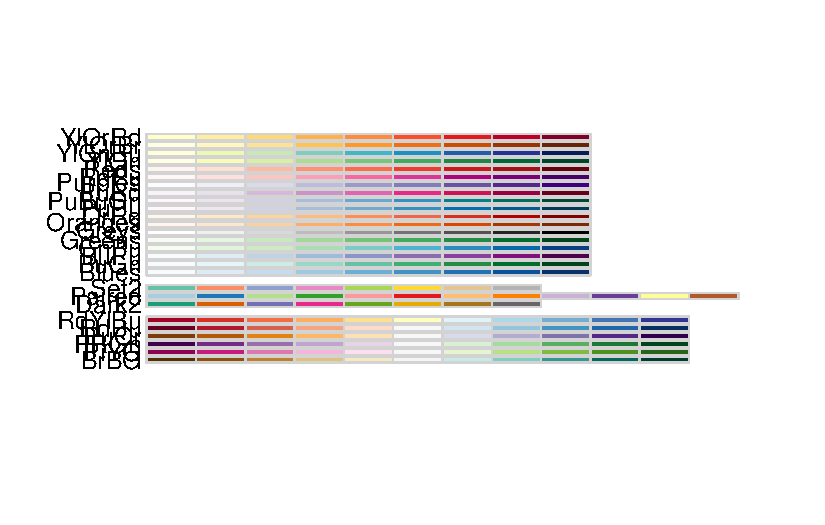
\includegraphics{./pakker_files/figure-pdf/unnamed-chunk-4-1.pdf}

}

\end{figure}

Det siste jeg sa er forresten ikke helt sant. Du kan kjøre en funksjon
fra en pakke uten å ha lasta den inn. Da skriver du navnet på pakka,
etterfult av to kolon og så navnet på funksjonen.

\begin{Shaded}
\begin{Highlighting}[]
\NormalTok{RColorBrewer}\SpecialCharTok{::}\FunctionTok{display.brewer.pal}\NormalTok{(}\AttributeTok{n =} \DecValTok{8}\NormalTok{, }\AttributeTok{name =} \StringTok{\textquotesingle{}Dark2\textquotesingle{}}\NormalTok{)}
\end{Highlighting}
\end{Shaded}

\begin{figure}[H]

{\centering 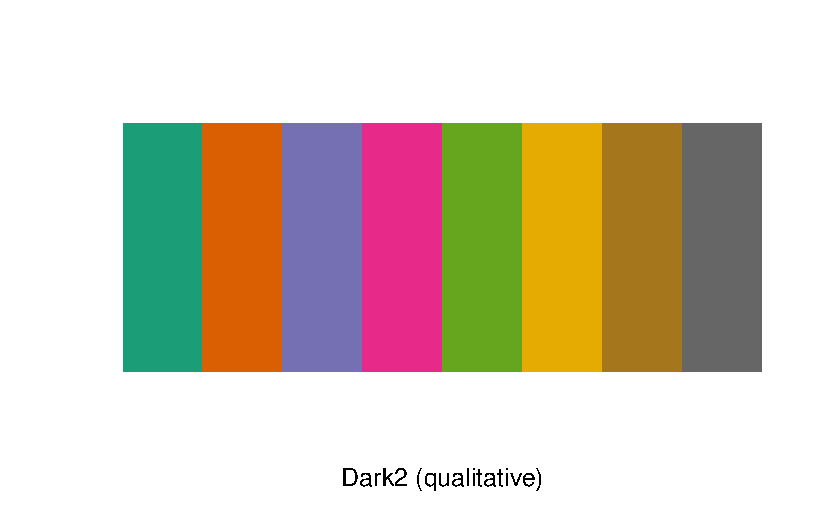
\includegraphics{./pakker_files/figure-pdf/unnamed-chunk-5-1.pdf}

}

\end{figure}

Så lenge pakka er lasta inn kan jeg bruke alle funksjonene fra pakka.
Noen ganger trenger jeg bare én funksjon fra en pakke, og da benytter
jeg meg av det over istedenfor å laste inn hele pakka.

\hypertarget{tidyverse}{%
\section{Tidyverse}\label{tidyverse}}

Tidyverse refererer til

\begin{itemize}
\tightlist
\item
  en designfilosofi
\item
  en stor gruppe med pakker
\item
  en spesifikk pakke som grupperer et lite antall pakker
\end{itemize}

Du kan lese mer om \href{https://www.tidyverse.org/}{Tidyverse på
nettsida deres}. Det er også en lærebok som går grundigere gjennom alle
funksjonene deres, \href{https://r4ds.had.co.nz/}{R for Data Science}.

\begin{figure}

{\centering 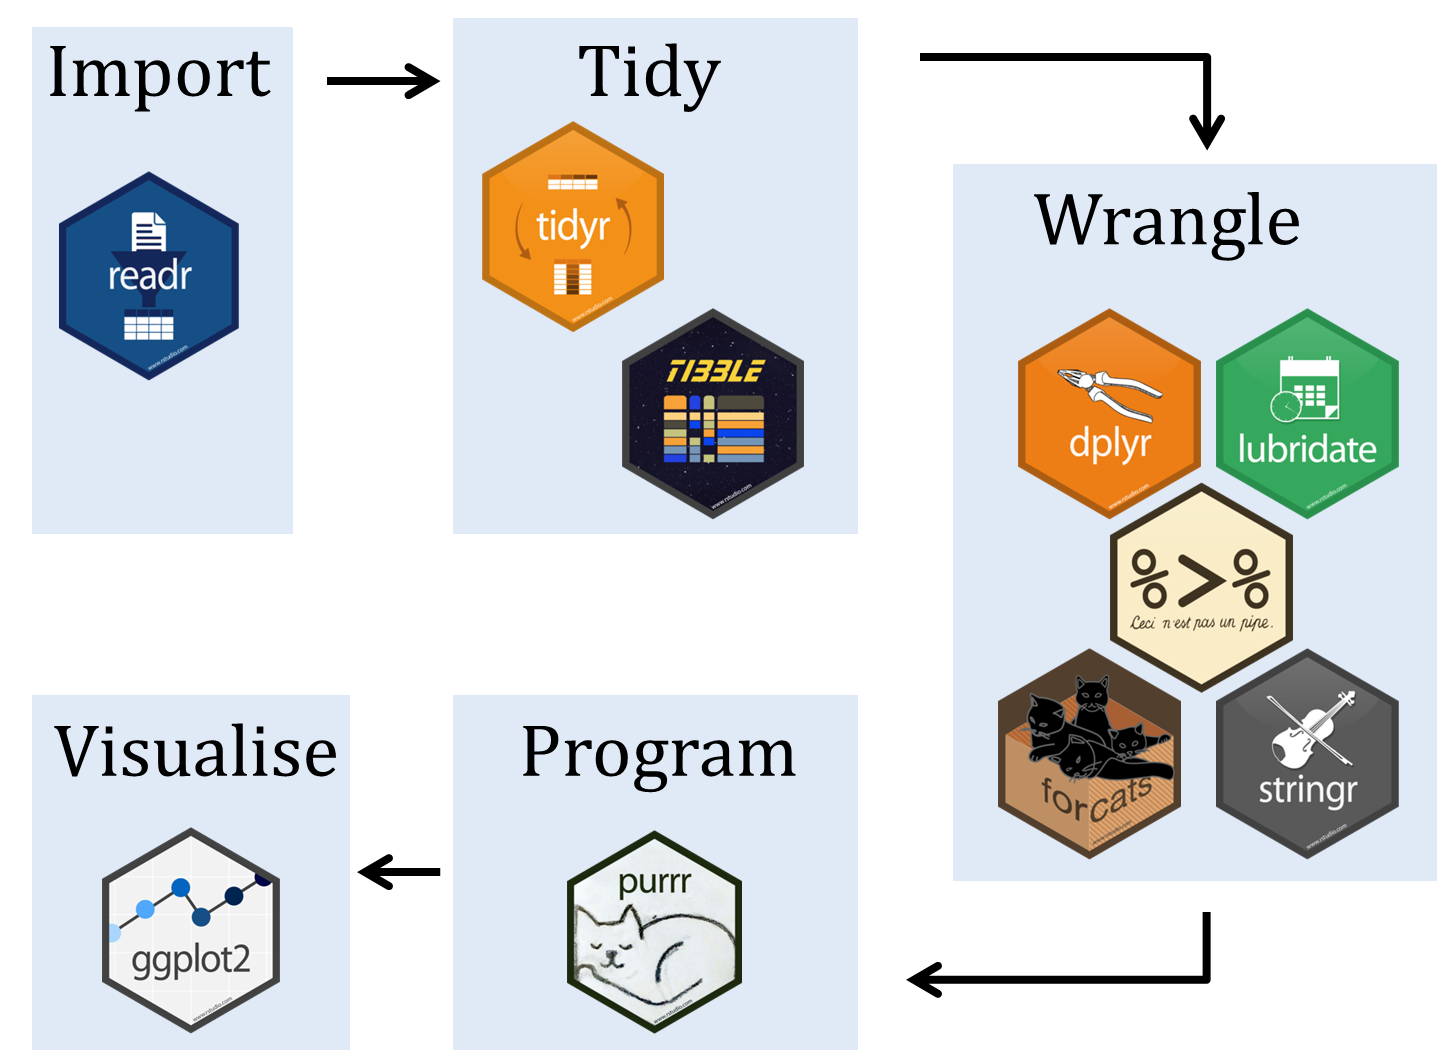
\includegraphics[width=0.7\textwidth,height=\textheight]{./img/tidy_workflow.png}

}

\caption{Tidyverse. Fra http://www.seec.uct.ac.za/r-tidyverse}

\end{figure}

Når man kjører \texttt{library(tidyverse)} vil den laste inn alle
pakkene nevnt \href{https://www.tidyverse.org/packages/}{her}. Blant
annet \texttt{dplyr}, \texttt{ggplot2}, etc. I tillegg laster den inn
enkeltfunksjoner fra andre pakker. F.eks. laster den inn pipe operatoren
( \texttt{\%\textgreater{}\%}) fra \texttt{magrittr}. Mer om den
seinere. Dermed er dette egentlig en snarvei for å slippe å laste inn
flere pakker.

Tidyverse-pakkene er designa for å harmonisere med hverandre, og det
gjør dem veldig sterke. Den underliggende filosofien gir også et bra
rammeverk for andre pakker. Vinn-vinn.

Reint praktisk er det sånn at mange av funksjonene i \texttt{tidyverse}
allerede eksisterer i \texttt{base\ R}. F.eks. filtrering, mutering, og
etter \texttt{R\ v.4.1.}, pipe-funksjonen. Jeg bruker likevel
\texttt{tidyverse}-variantene fordi disse er så mye lettere å forstå,
skrive, og lese. De er utvikla for folk som jobber som oss, med tabeller
og datasett. Som nybegynner er det ikke bare bare å forstå forskjellen
mellom \texttt{base\ R} og \texttt{tidyverse}, så her er det viktigste:

\begin{itemize}
\tightlist
\item
  Når dere søker opp løsninger vil det ofte presenteres løsninger både i
  \texttt{base\ R} og i \texttt{tidyverse}. Dette skjer ofte på
  StackOverflow.
\item
  De fleste \texttt{tidyverse}-funksjoner har et datasett som første
  argument i funksjonen. Dette gjør at vi lett kan \emph{pipe}
  funksjoner etter hverandre.
\end{itemize}

\hypertarget{piper}{%
\section{Piper}\label{piper}}

Hvorfor er piper så nyttig? De lar oss flette sammen en serie
operasjoner uten å måtte mellomlagre objekter. La oss si at vi har et
datasett med biler og deres egenskaper. Vi vil

\begin{itemize}
\tightlist
\item
  filtrere ut dem som har under seks sylindre
\item
  gjøre om vekta fra lbs. til kg.
\item
  gruppere etter antall gir
\item
  vise snitt av miles/gallon (mpg).
\end{itemize}

\hypertarget{uten-pipe}{%
\subsection{Uten pipa}\label{uten-pipe}}

\begin{Shaded}
\begin{Highlighting}[]
\FunctionTok{library}\NormalTok{(tidyverse)}
\end{Highlighting}
\end{Shaded}

\begin{verbatim}
-- Attaching packages --------------------------------------- tidyverse 1.3.2 --
v ggplot2 3.3.6      v purrr   0.3.5 
v tibble  3.1.8      v dplyr   1.0.10
v tidyr   1.2.1      v stringr 1.4.1 
v readr   2.1.3      v forcats 0.5.2 
-- Conflicts ------------------------------------------ tidyverse_conflicts() --
x dplyr::filter() masks stats::filter()
x dplyr::lag()    masks stats::lag()
\end{verbatim}

\begin{Shaded}
\begin{Highlighting}[]
\NormalTok{mtcars }\OtherTok{\textless{}{-}}\NormalTok{ mtcars}
\NormalTok{cars\_filtered }\OtherTok{\textless{}{-}} \FunctionTok{filter}\NormalTok{(mtcars, cyl }\SpecialCharTok{\textgreater{}=} \DecValTok{6}\NormalTok{)}
\NormalTok{cars\_filtered\_kg }\OtherTok{\textless{}{-}} \FunctionTok{mutate}\NormalTok{(cars\_filtered, }\AttributeTok{wt =}\NormalTok{ wt }\SpecialCharTok{*} \FloatTok{0.45359237}\NormalTok{)}
\NormalTok{cars\_filtered\_kg\_grouped }\OtherTok{\textless{}{-}} \FunctionTok{group\_by}\NormalTok{(cars\_filtered\_kg, gear)}
\NormalTok{cars\_filtered\_kg\_grouped\_mean }\OtherTok{\textless{}{-}} \FunctionTok{summarise}\NormalTok{(cars\_filtered\_kg\_grouped, }\AttributeTok{snitt =} \FunctionTok{mean}\NormalTok{(mpg))}

\NormalTok{cars\_filtered\_kg\_grouped\_mean}
\end{Highlighting}
\end{Shaded}

\begin{verbatim}
# A tibble: 3 x 2
   gear snitt
  <dbl> <dbl>
1     3  15.7
2     4  19.8
3     5  16.8
\end{verbatim}

\hypertarget{med-pipe}{%
\subsection{Med pipa}\label{med-pipe}}

\begin{Shaded}
\begin{Highlighting}[]
\FunctionTok{library}\NormalTok{(tidyverse)}
\NormalTok{cars\_filtered\_kg\_group\_mean }\OtherTok{\textless{}{-}}\NormalTok{ mtcars }\SpecialCharTok{\%\textgreater{}\%} 
  \FunctionTok{filter}\NormalTok{(cyl }\SpecialCharTok{\textgreater{}=} \DecValTok{6}\NormalTok{) }\SpecialCharTok{\%\textgreater{}\%} 
  \FunctionTok{mutate}\NormalTok{(}\AttributeTok{wt =}\NormalTok{ wt }\SpecialCharTok{*} \FloatTok{0.45359237}\NormalTok{) }\SpecialCharTok{\%\textgreater{}\%} 
  \FunctionTok{group\_by}\NormalTok{(gear) }\SpecialCharTok{\%\textgreater{}\%} 
  \FunctionTok{summarise}\NormalTok{(}\AttributeTok{snitt =} \FunctionTok{mean}\NormalTok{(mpg))}

\NormalTok{cars\_filtered\_kg\_grouped\_mean}
\end{Highlighting}
\end{Shaded}

\begin{verbatim}
# A tibble: 3 x 2
   gear snitt
  <dbl> <dbl>
1     3  15.7
2     4  19.8
3     5  16.8
\end{verbatim}

Det andre eksemplet er

\begin{enumerate}
\def\labelenumi{\arabic{enumi}.}
\tightlist
\item
  mer lesbart
\item
  mindre stappfult av midlertidige objekter som vi seinere må slette
  eller som uansett overskriver hverandre.
\end{enumerate}

Jeg kommer til å bruke piper en god del både her og i alle skriptene
mine. Så det er greit å vite hva det går ut på. Syntaksen
\texttt{x\ \%\textgreater{}\%\ y} kan leses som \texttt{y\ får\ x}. Vi
tar \texttt{x} og sender det til \texttt{y} som tar det inn som sitt
første \emph{argument}. Tidyverse-funksjonene er bygd rundt ideen om at
det første argumentet til funksjonene er et datasett. Legg merke til at
det er et datasett som er det første objektet i alle funksjonen jeg
bruker i eksemplet uten pipe.

Noen funksjoner, som \texttt{base::sum()} har ikke data som sitt første
argument, men en vektor. Hvis man sender et datasett til \texttt{sum()}
vil man få en feilmelding.

\begin{Shaded}
\begin{Highlighting}[]
\NormalTok{mtcars }\SpecialCharTok{\%\textgreater{}\%} \FunctionTok{sum}\NormalTok{(wt)}
\end{Highlighting}
\end{Shaded}

\begin{verbatim}
Error in mtcars %>% sum(wt): object 'wt' not found
\end{verbatim}

For å få slike funksjoner til å funkere med ei pipe, kan man ofte bruke
en funksjon fra \texttt{magrittr}:

\begin{Shaded}
\begin{Highlighting}[]
\NormalTok{mtcars }\SpecialCharTok{\%\textgreater{}\%} \FunctionTok{sum}\NormalTok{(.}\SpecialCharTok{$}\NormalTok{wt)}
\end{Highlighting}
\end{Shaded}

\begin{verbatim}
[1] 14045.15
\end{verbatim}

\texttt{.} blir her et alias for det aktuelle datasett, og dette er det
samme som å skrive:

\begin{Shaded}
\begin{Highlighting}[]
\FunctionTok{sum}\NormalTok{(mtcars}\SpecialCharTok{$}\NormalTok{wt)}
\end{Highlighting}
\end{Shaded}

\begin{verbatim}
[1] 102.952
\end{verbatim}

Da jeg lærte R var det \texttt{\%\textgreater{}\%} fra \texttt{magrittr}
som var den gjeldende pipa. Den var så nyttig at ei pipe til slutt blei
inkorporert i \texttt{base\ R}. Dette skjedde i \texttt{R\ 4.1.0}.
\texttt{Base\ R}s pipe ser slik ut: \texttt{\textbar{}\textgreater{}}.
Den fungerer i hovedsak lik \texttt{\%\textgreater{}\%}. Når jeg
fortsetter å bruke den gamle \texttt{magrittr}-pipa er det bare fordi
jeg er gammel og ikke liker å endre på ting som funker. Dessuten har
Rstudio en flott snarvei til \texttt{\%\textgreater{}\%} via
\texttt{ctrl\ +\ shift\ +\ M}.

Dere velger altså sjøl om dere går for \texttt{\%\textgreater{}\%} eller
\texttt{\textbar{}\textgreater{}}. Husk bare at for å bruke
\texttt{\%\textgreater{}\%} så må \texttt{tidyverse} eller
\texttt{magrittr} lastes inn først. (\texttt{tidyverse} låner noen av
funksjonene fra \texttt{magrittr}, men laster ikke inn \emph{alle}
funksjonene fra den pakka).

\hypertarget{hva-er-pipa-ikke}{%
\subsection{Hva er pipa ikke?}\label{hva-er-pipa-ikke}}

En vanlig intuisjon man får når man begynner med piper er at det er en
måte å ``arbeide baklengs''. Man starter å lese nedenfra og opp. Dette
stemmer ikke. Tenk heller at du starter med en ting, sender den videre
til en funksjon, og sender \emph{resultatet av dette videre} til neste
funksjon, sender resultatet av dette videre til neste funksjon, og så
videre.

\bookmarksetup{startatroot}

\hypertarget{grunnleggende}{%
\chapter{Det grunnleggende}\label{grunnleggende}}

Vi starter gradvis på bunnen og arbeider oss kjapt opp til den avanserte
arbeidsflyten vi er vant med. Det vil si at vi starter med enkle lister
og datasett. Så forlater vi dette og jobber kun med datasett.

\begin{Shaded}
\begin{Highlighting}[]
\CommentTok{\# Laster inn tidyverse, som vi alltid bruker}
\FunctionTok{library}\NormalTok{(tidyverse)}
\end{Highlighting}
\end{Shaded}

\begin{verbatim}
-- Attaching packages --------------------------------------- tidyverse 1.3.2 --
v ggplot2 3.3.6      v purrr   0.3.5 
v tibble  3.1.8      v dplyr   1.0.10
v tidyr   1.2.1      v stringr 1.4.1 
v readr   2.1.3      v forcats 0.5.2 
-- Conflicts ------------------------------------------ tidyverse_conflicts() --
x dplyr::filter() masks stats::filter()
x dplyr::lag()    masks stats::lag()
\end{verbatim}

\hypertarget{sec-rstudio}{%
\section{Rstudio}\label{sec-rstudio}}

Men først av alt bør vi ta en titt på Rstudio. Dette er som nevnt det
grafiske brukergrensesnittet som vi arbeider i når vi jobber med R. Et
typisk Rstudio-vindu kan se slik ut:

\begin{figure}

{\centering 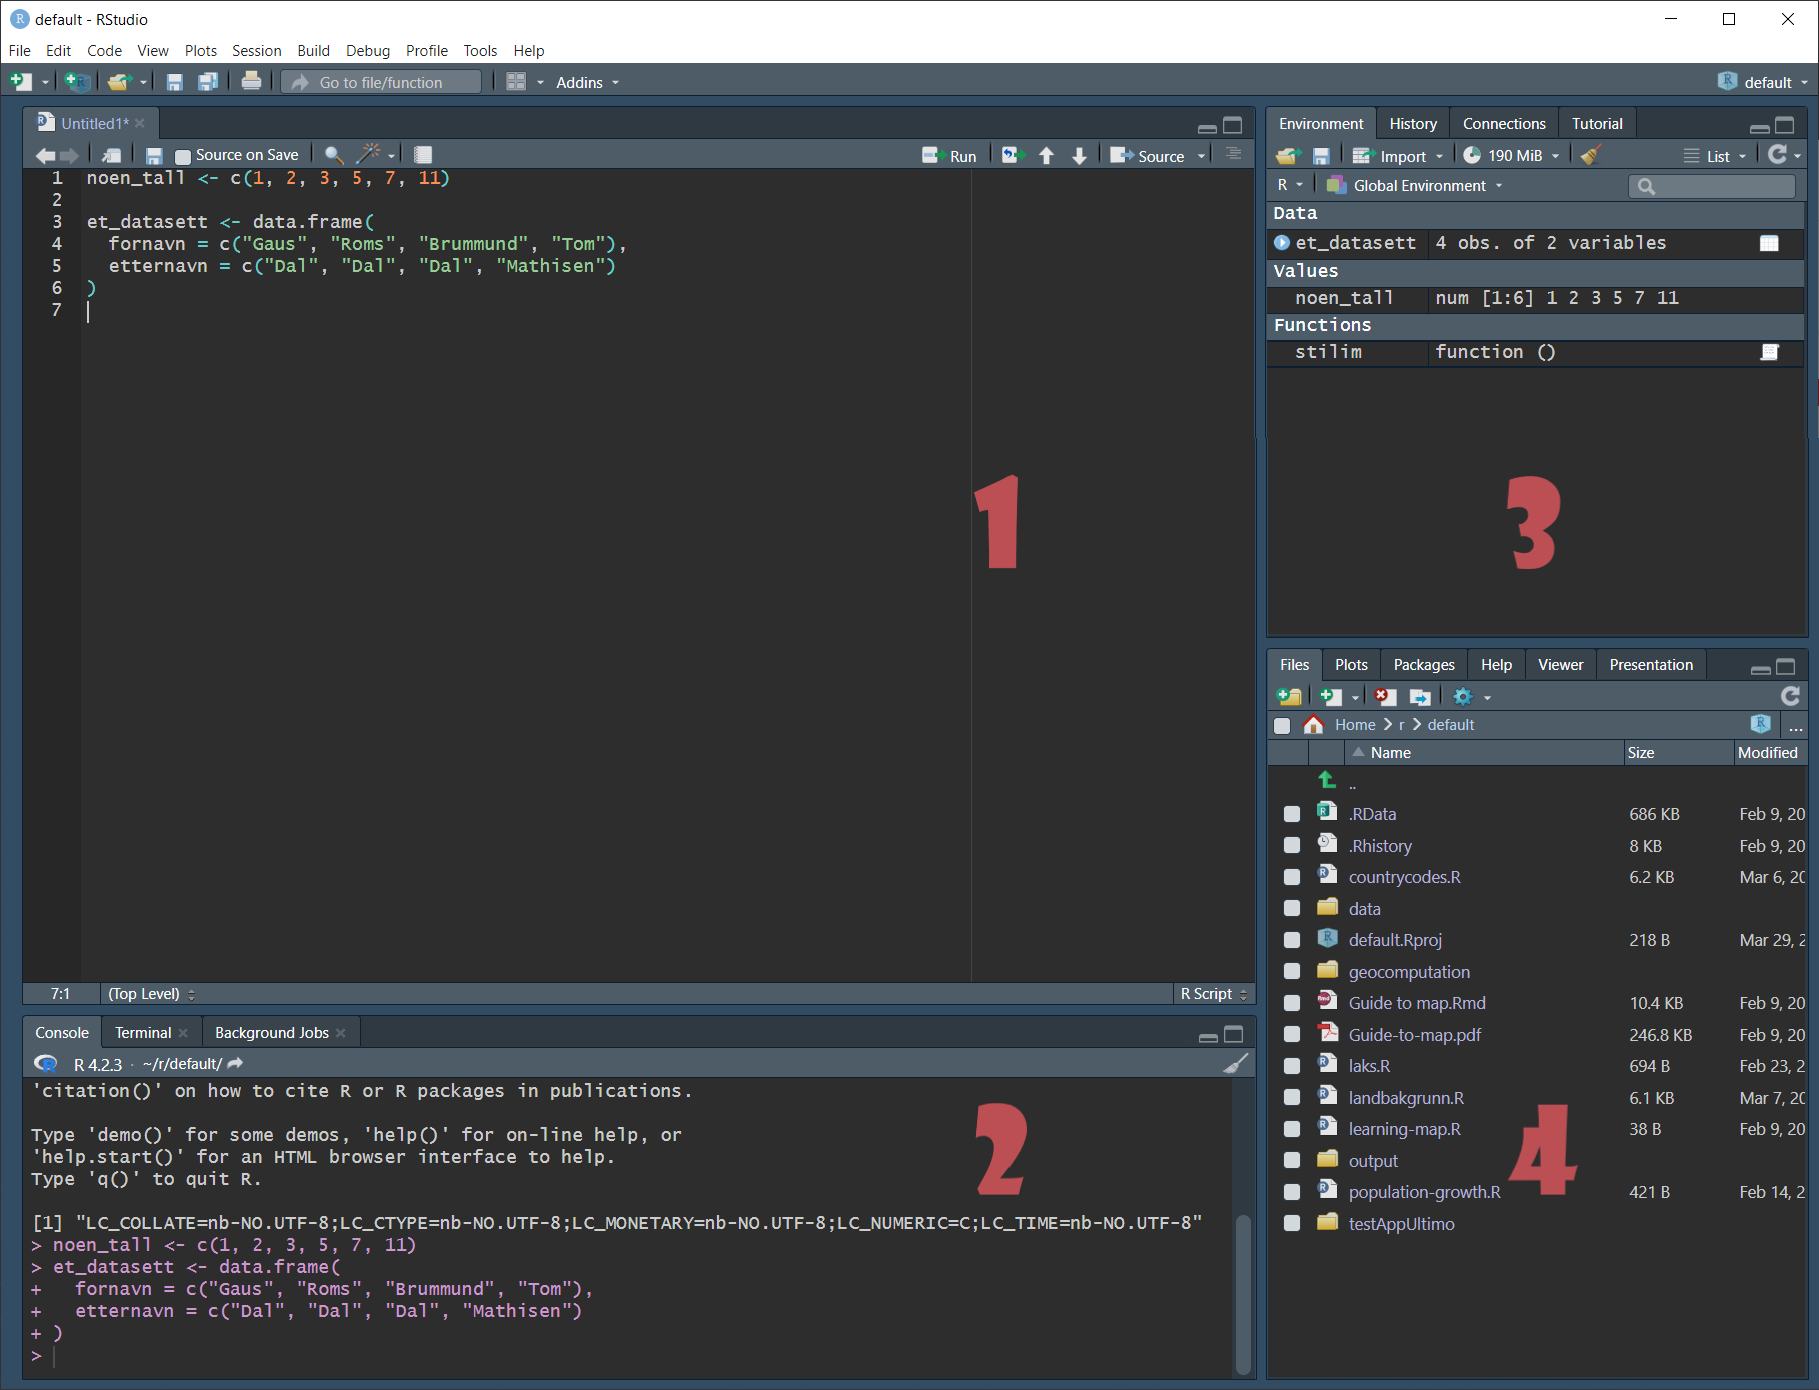
\includegraphics{./img/rstudio_annotated.PNG}

}

\caption{Rstudio in action, med tema \emph{Tomorrow Night 80s}}

\end{figure}

Hvis du har kjedeligere farger er det nok fordi du ikke har oppdaga de
flotte temaene som du kan velge mellom i Rstudio. Kikk på
\emph{Tools/Global options/Appearance} og endre \emph{Editor theme} til
noe som faller deg i smak. Min favoritt for tida er \emph{Tomorrow Night
80s}. Grensesnittet består av fire ruter (\emph{panes}), som hver kan ha
flere faner (\emph{tabs}).

Når du først er i innstillinger: Skru av \emph{Restore .RData into
workspace on startup} og velg \emph{never} på \emph{Save workspace to
.RData on exit}. Dette er innstillinger som gjør det litt raskere for
deg å komme inn i et prosjekt, men som vil gi deg en falsk trygghet, og
som inviterer til noen av de feilene om jeg omtaler i
Chapter~\ref{sec-feil}. Derfor skrur vi dem av.\footnote{Hvorfor skrur
  vi av dette? Innstillinga er på \emph{by default} og vil lagre alt som
  ligger i miljøet ditt mellom hver gang du jobber i Rstudio, sjøl om du
  lukker programmet og skrur av maskina. Dette gjør det som nevnt
  lettere å starte opp igjen. Samtidig fører det til at miljøet ditt
  blir overfylt av gamle objekter og pakker du har lasta inn. Du kommer
  til å på et tidspunkt få en feil fordi du har lasta inn en gammel
  pakke du hadde glemt, eller fordi det ligger et objekt i miljøet du
  hadde glemt av. Det er god hygiene å restarte sesjonen ofte (flere
  ganger i løpet av et prosjekt), og denne innstillinga er med på å
  hindre deg i å gjøre det.}

\begin{figure}

{\centering 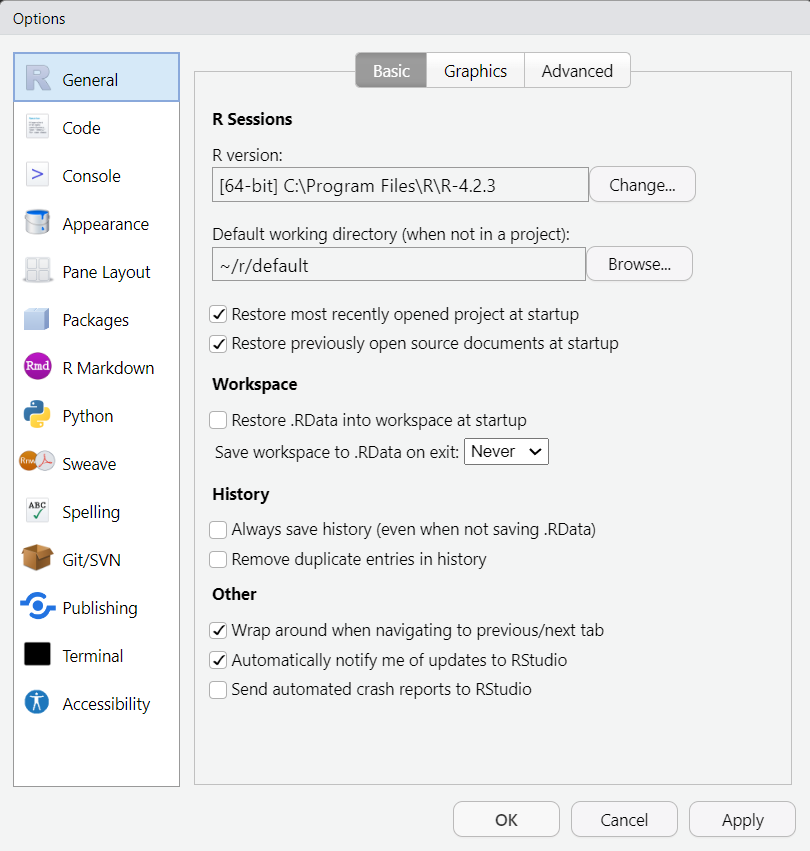
\includegraphics[width=0.5\textwidth,height=\textheight]{./img/settings.png}

}

\caption{Slik skal det se ut}

\end{figure}

\hypertarget{rute-1-kilde-source}{%
\subsection{\texorpdfstring{Rute 1: Kilde
(\emph{source})}{Rute 1: Kilde (source)}}\label{rute-1-kilde-source}}

I denne ruta havner alle skriptene våre. Vi skriver alle kommandoene
våre i skript som vi deretter kjører. Dette er likt hvordan
syntaks/skript kan brukes i Stata og SPSS. Disse skripta blir en
oppskrift for oss seinere som forteller oss hva som blei gjort. Du kan
kjøre ei og ei linje ved å trykke \texttt{ctrl\ +\ enter}\footnote{For
  macOS-brukere: erstatt \texttt{ctrl} med \texttt{cmd} i disse
  snarveiene.}, eller du kan markere det du vil kjøre og trykke det
samme. Du kan kjøre hele skriptet ved å trykke
\texttt{ctrl\ +\ alt\ +\ enter}. Skript lar deg enkelt dele arbeidet
ditt med andre. Du bør være flink på å \emph{dokumentere} det du gjør
ved å bruke kommentarer. Dette er linjer som starter med \texttt{\#}.
Disse linjene vil ignoreres av R når du kjører skriptet.

Du kan se at jeg har skrevet noe kode i skriptet mitt. Jeg lager en
vektor som heter \emph{noen\_tall} og et datasett som heter
\emph{et\_datasett}.

\hypertarget{rute-2-konsollen-console}{%
\subsection{\texorpdfstring{Rute 2: Konsollen
(\emph{console})}{Rute 2: Konsollen (console)}}\label{rute-2-konsollen-console}}

Man kan også skrive kommandoer rett til konsollen. Da blir de kjørt med
en gang man trykker \texttt{enter}. De kodene du skriver til konsollen
vil ikke bli lagra noe sted, så hvis du jobber mye her vil du ikke
dokumentere arbeidet ditt. Så ikke gjør det til en vane å bruke
konsollen mye. Den er nyttig hvis du veit at du ikke trenger å ta vare
på akkurat det du gjør nå. F.eks. hvis du skal regne ut noe fort, eller
printe et objekt for å inspisere det.

Når du kjører skript vil koden skrives ut til konsollen. Du kan se at
jeg har kjørt kodene i skriptet fordi de er blitt skrevet til konsollen.

\hypertarget{rute-3-miljuxf8et-environment-med-mer}{%
\subsection{\texorpdfstring{Rute 3: Miljøet (\emph{environment}) med
mer}{Rute 3: Miljøet (environment) med mer}}\label{rute-3-miljuxf8et-environment-med-mer}}

De to siste rutene kan inneholde diverse faner, avhengig av hva du
krysser av for i \emph{Pane layout} i \emph{global options}. Vanligvis
viser det oss miljøet vårt. Her finner du en oversikt over alle
objektene du har laga hittil i \textbf{sesjonen} (\emph{session}) din.
En sesjon starter når du starter R (som starter når du starter Rstudio).
Den varer til du skrur av R eller restarter den manuelt. Du restarter
den manuelt ved å gå til \emph{Session/Restart R} eller trykke
\texttt{ctrl\ +\ shift\ +\ F10}.

Du kan se at det ligger en vektor, et datasett og en funksjon
(\emph{stilim()}) i mijøet mitt. De to første er det jeg lagde i
skriptet. Da koden blei kjørt lagde de to \textbf{objekter} (et datasett
og en vektor), og alle objekter legges i miljøet. Funksjonen ligger der
fordi den er definert i min \emph{.Rprofile}. Dette går jeg ikke inn på
her, for det er et mer avansert tema. Det holder å si at denne
funksjonen blir lasta inn i miljøet mitt hver gang jeg starter en
R-sesjon.

Det er andre faner i denne ruta som kan være nyttig, men vi trenger ikke
bry oss om dem nå. Kort fortalt viser \emph{History} oss hvilke koder vi
nettopp har kjørt, og Git kan brukes hvis vi bruker Git som et
\emph{version control system.}

\hypertarget{rute-4-filer-plott-visning-hjelp-med-mer}{%
\subsection{Rute 4: Filer, plott, visning, hjelp med
mer}\label{rute-4-filer-plott-visning-hjelp-med-mer}}

Her ligger det flere faner som er interessant for oss.

\hypertarget{files}{%
\subsubsection{Files}\label{files}}

Vanligvis ser vi filene i den mappa vi befinner oss her, hvis fana
\emph{Files} er valgt. Her ligger alle filene jeg har i min mappe for
øyeblikket. Det er noe rotete. Herfra kan du enkelt åpne andre skript.

\hypertarget{plots}{%
\subsubsection{Plots}\label{plots}}

Hvis du lager en figur eller graf vil plottet kunne vises her.

\hypertarget{help}{%
\subsubsection{Help}\label{help}}

Lær å like \emph{Help}. Her kan du søke opp funksjoner for å få hjelp
til å bruke dem. Du kan enten bruke søkefeltet i høyre hjørne av fana,
eller kjøre denne koden \texttt{?funksjonsnavn}. F.eks.

\begin{Shaded}
\begin{Highlighting}[]
\NormalTok{?mutate}
\end{Highlighting}
\end{Shaded}

Da vil hjelpevinduet dukke opp.

\hypertarget{viewer}{%
\subsubsection{Viewer}\label{viewer}}

\emph{Viewer} lar oss forhåndsvise f.eks. html-sider, Shiny-apps og
andre dokumenter vi produserer.

\hypertarget{vektor}{%
\section{Vektor}\label{vektor}}

Det grunnleggende elementet i R er en \textbf{vektor}. En vektor kan
forstås som en liste av elementer med samme type. Vi kan ha vektorer av
tall, bokstaver, faktorer. De tre siste er eksempler på klasser. Det er
noen forskjellige klasser, men vi bryr oss mest om disse tre.

La oss lage en vektor

\begin{Shaded}
\begin{Highlighting}[]
\FunctionTok{c}\NormalTok{(}\DecValTok{1}\NormalTok{, }\DecValTok{2}\NormalTok{, }\DecValTok{3}\NormalTok{)}
\end{Highlighting}
\end{Shaded}

\begin{verbatim}
[1] 1 2 3
\end{verbatim}

Funksjonen \texttt{c()} kombinerer verdier til en vektor.

Når vi skriver en kommando vil R alltid returnere noe til oss. Det blir
vanligvis printa til skjermen. Hvis vi heller vi lagre det som et objekt
som vi kan henvise til seinere, bruker vi \texttt{assignment} for å
\textbf{gi} verdien(e) til et objekt vi navngir.

Slik:

\begin{Shaded}
\begin{Highlighting}[]
\NormalTok{vektor1 }\OtherTok{\textless{}{-}} \FunctionTok{c}\NormalTok{(}\DecValTok{1}\NormalTok{, }\DecValTok{2}\NormalTok{, }\DecValTok{3}\NormalTok{)}
\NormalTok{vektor1}
\end{Highlighting}
\end{Shaded}

\begin{verbatim}
[1] 1 2 3
\end{verbatim}

\begin{tcolorbox}[enhanced jigsaw, breakable, colframe=quarto-callout-note-color-frame, rightrule=.15mm, arc=.35mm, toprule=.15mm, bottomrule=.15mm, toptitle=1mm, colback=white, opacitybacktitle=0.6, left=2mm, titlerule=0mm, title=\textcolor{quarto-callout-note-color}{\faInfo}\hspace{0.5em}{Note}, colbacktitle=quarto-callout-note-color!10!white, bottomtitle=1mm, coltitle=black, leftrule=.75mm, opacityback=0]

Når man gir en verdi bruker man en av to operatorer: enten
\texttt{\textless{}-} eller \texttt{=}. Det er generelt ansett at man
bør bruke pila istedenfor likhetstegn. Årsakene er

\begin{enumerate}
\def\labelenumi{\arabic{enumi}.}
\tightlist
\item
  \texttt{=} (\emph{assignment}) er lett å forveksle med \texttt{==}
  (\emph{comparison}). Det er enklere å unngå dette med pila
\item
  pila er anvendelig. Du kan faktisk skrive den motsatt vei, slik:
  \texttt{c(1,\ 2,\ 3)\ -\textgreater{}\ vektor1}. Når det er sagt, lov
  meg at du aldri gjør dette med mindre du har en utrolig god grunn.
  Enkelte konvensjoner er smart å beholde.
\end{enumerate}

Derfor bruker jeg alltid \texttt{\textless{}-}, og anbefaler deg det
også.

\end{tcolorbox}

Tall kan man, som vi ser, bare skrive rett ut. Bokstaver, derimot, må
deklareres som en \textbf{streng}. Dette gjøres ved å omkranse dem i
hermetegn:

\begin{Shaded}
\begin{Highlighting}[]
\NormalTok{vektor2 }\OtherTok{\textless{}{-}} \FunctionTok{c}\NormalTok{(}\StringTok{"A"}\NormalTok{, }\StringTok{"B"}\NormalTok{, }\StringTok{"C"}\NormalTok{)}
\NormalTok{vektor2}
\end{Highlighting}
\end{Shaded}

\begin{verbatim}
[1] "A" "B" "C"
\end{verbatim}

En vektor som består av bokstaver eller ord kalles en \emph{character
vector} eller en \emph{string}.

Vi kommer oss langt med numeriske vektorer og strengvektorer. Her er det
verdt å merke at det er forskjellige varianter av numeriske vektorer: De
kan være \texttt{Int}, \texttt{double}, eller \texttt{float}.
Forskjellen er sjelden viktig for oss, så jeg går ikke inn på det.

Mer inngående info om vektorer og klasser
\href{https://r02pro.github.io/vector.html}{kan finnes her}.

En vektor kan bestå av alt fra ett til mange elementer. \textbf{Men den
kan bare bestå av elementer av samme klasse}

La oss se kjapt på andre typer dataverdier vi kan arbeide med.

\hypertarget{datoer}{%
\subsection{Datoer}\label{datoer}}

Datoer er spesielle verdier i R. Dette lar oss gjøre spesielle ting som
å regne ut tidsdifferansen mellom to datoer i dager, måneder eller år,
og mange andre nyttige ting. Pakka \texttt{lubridate} inneholder mange
nyttige funksjoner som utvider de som ligger i \texttt{base\ R}. Er
\texttt{lubridate} en del av \texttt{tidyverse}? Så klart.

\hypertarget{logiske-verdier}{%
\subsection{Logiske verdier}\label{logiske-verdier}}

Det er også verdt å være oppmerksom på logiske vektorer. Elementer i
disse vektorene kan kun være \emph{enten} \texttt{TRUE} (sann) eller
\texttt{FALSE} (usann). De brukes mye i filtrering og testing.

\hypertarget{missing-na}{%
\subsection{Missing (NA)}\label{missing-na}}

Det siste typen element vi må huske på er missing. Alle dataprogrammer
har ulik måte å lagre såkalte \emph{missing data} på. I R vises de som
\texttt{NA}. Det er masse vi kunne sagt om \texttt{NA}, mer enn jeg
rekker her. Jeg nevner kjapt: En del funksjoner, spesielt i
\texttt{base\ R} liker ikke missing. Blant annet \texttt{sum()}. Den vil
gi \texttt{NA} som svar dersom det er missing tilstede i datasettet,
hvilket aldri er det vi forventer oss. Disse funksjonene har alltid
mulighet til å \emph{ignorere} missing ved å sette et spesielt argument.
F.eks. \texttt{na.rm\ =\ TRUE}

\begin{Shaded}
\begin{Highlighting}[]
\CommentTok{\# En tilfeldig vektor med missing}
\NormalTok{foo }\OtherTok{\textless{}{-}} \FunctionTok{c}\NormalTok{(}\DecValTok{1}\NormalTok{, }\DecValTok{2}\NormalTok{, }\DecValTok{3}\NormalTok{, }\ConstantTok{NA}\NormalTok{)}

\CommentTok{\# Forventer 6, får NA.}
\FunctionTok{sum}\NormalTok{(foo)}
\end{Highlighting}
\end{Shaded}

\begin{verbatim}
[1] NA
\end{verbatim}

\begin{Shaded}
\begin{Highlighting}[]
\CommentTok{\# Slik ber vi sum ignorere missing.}
\FunctionTok{sum}\NormalTok{(foo, }\AttributeTok{na.rm =} \ConstantTok{TRUE}\NormalTok{)}
\end{Highlighting}
\end{Shaded}

\begin{verbatim}
[1] 6
\end{verbatim}

Når vi importerer filer fra andre programmer hender det vi får med oss
deres definisjon av missing. F.eks. er missing noen ganger koda som
\texttt{-999} i SPSS-filer. Her kan det skje feil slik at disse verdiene
blir til \texttt{999} i R. Det skjer sjelden, men det er verdt å være
oppmerksom på muligheten for at det skjer.

\hypertarget{faktor}{%
\subsection{Faktor}\label{faktor}}

Faktorer (\emph{factors}) må også nevnes. Disse er nyttige for
grupperinger, og noen funksjoner kan merke seg hvilke variabler som er
faktorer og utføre heuristikker basert på det. Sjøl syns jeg faktorer er
knotete å forholde seg til, så jeg foretrekker å bare bruke
strengvektorer.

\hypertarget{liste}{%
\section{Liste}\label{liste}}

En liste er som en vektor på steroider. Den kan består av elementer av
\emph{ulik klasse}. I tillegg kan en liste bestå av \emph{andre lister}.
Det gjør dem kraftig, og anvendbar.

\begin{Shaded}
\begin{Highlighting}[]
\CommentTok{\# En liste bestående av fem tall. Dette kunne like gjerne vært en vektor}
\NormalTok{liste1 }\OtherTok{\textless{}{-}} \FunctionTok{list}\NormalTok{(}\DecValTok{1}\NormalTok{, }\DecValTok{2}\NormalTok{, }\DecValTok{3}\NormalTok{, }\DecValTok{4}\NormalTok{, }\DecValTok{5}\NormalTok{)}
\NormalTok{liste1}
\end{Highlighting}
\end{Shaded}

\begin{verbatim}
[[1]]
[1] 1

[[2]]
[1] 2

[[3]]
[1] 3

[[4]]
[1] 4

[[5]]
[1] 5
\end{verbatim}

\begin{Shaded}
\begin{Highlighting}[]
\CommentTok{\# Denne lista har elementer av ulik klasse.}
\NormalTok{liste1 }\OtherTok{\textless{}{-}} \FunctionTok{list}\NormalTok{(}\DecValTok{1}\NormalTok{, }\StringTok{"B"}\NormalTok{, }\DecValTok{3}\NormalTok{, }\StringTok{"D"}\NormalTok{, }\DecValTok{5}\NormalTok{)}
\NormalTok{liste1}
\end{Highlighting}
\end{Shaded}

\begin{verbatim}
[[1]]
[1] 1

[[2]]
[1] "B"

[[3]]
[1] 3

[[4]]
[1] "D"

[[5]]
[1] 5
\end{verbatim}

\begin{Shaded}
\begin{Highlighting}[]
\CommentTok{\# En liste bestående av flere vektorer og lister. }
\NormalTok{liste2 }\OtherTok{\textless{}{-}} \FunctionTok{list}\NormalTok{(}
  \AttributeTok{vektorA =} \FunctionTok{c}\NormalTok{(}\DecValTok{1}\NormalTok{, }\DecValTok{2}\NormalTok{, }\DecValTok{3}\NormalTok{, }\DecValTok{4}\NormalTok{),}
  \AttributeTok{vektorB =} \FunctionTok{c}\NormalTok{(}\StringTok{"ET"}\NormalTok{, }\StringTok{"IJ"}\NormalTok{, }\StringTok{"SW"}\NormalTok{), }
  \AttributeTok{liste1 =} \FunctionTok{list}\NormalTok{(}\DecValTok{3}\NormalTok{, }\DecValTok{4}\NormalTok{, }\DecValTok{5}\NormalTok{)}
\NormalTok{)}
\NormalTok{liste2}
\end{Highlighting}
\end{Shaded}

\begin{verbatim}
$vektorA
[1] 1 2 3 4

$vektorB
[1] "ET" "IJ" "SW"

$liste1
$liste1[[1]]
[1] 3

$liste1[[2]]
[1] 4

$liste1[[3]]
[1] 5
\end{verbatim}

Vi får direkte tilgang på elementene av objekter ved å bruke
firkantklammer (\texttt{{[}{]}}, a.k.a. hakeparentes, \emph{square
brackets}, \emph{box brackets}). Da bruker vi \emph{indeksen} til
elementet for å henvise til det. Indeksen er rekkefølga til elementet. R
er 1-indeksert. Det vil si at indeksen starter på 1. Andre
programmeringsspråk, slik som Python, starter på 0. Seinere skal vi se
at det går an å henvise til elementer ut fra \emph{navna} deres, men det
tar vi når vi kommer til det.

\begin{Shaded}
\begin{Highlighting}[]
\CommentTok{\# Hva er det første elementet i vektor1?}
\NormalTok{vektor1[}\DecValTok{1}\NormalTok{]}
\end{Highlighting}
\end{Shaded}

\begin{verbatim}
[1] 1
\end{verbatim}

\begin{Shaded}
\begin{Highlighting}[]
\CommentTok{\# Hva er det andre elementet i liste2?}
\NormalTok{liste2[}\DecValTok{2}\NormalTok{]}
\end{Highlighting}
\end{Shaded}

\begin{verbatim}
$vektorB
[1] "ET" "IJ" "SW"
\end{verbatim}

Spesielt når vi holder på med lister er det verdt å vite om dobbel
firkantklammer (\texttt{{[}{[}{]}{]}}). Vanlige firkantklammer gir deg
\emph{ei liste med element(ene) på denne indeksen}. Doble firkantklammer
gir deg \emph{sjølve element(ene) på denne indeksen}. Du kan se
forskjellen her:

\begin{Shaded}
\begin{Highlighting}[]
\CommentTok{\# Sjølve det som blir returnert.}
\NormalTok{liste2[}\DecValTok{2}\NormalTok{] }
\end{Highlighting}
\end{Shaded}

\begin{verbatim}
$vektorB
[1] "ET" "IJ" "SW"
\end{verbatim}

\begin{Shaded}
\begin{Highlighting}[]
\NormalTok{liste2[[}\DecValTok{2}\NormalTok{]]}
\end{Highlighting}
\end{Shaded}

\begin{verbatim}
[1] "ET" "IJ" "SW"
\end{verbatim}

\begin{Shaded}
\begin{Highlighting}[]
\CommentTok{\# Det blir tydeligere om vi undersøker klassen til objektene som blir returnert}
\NormalTok{liste2[}\DecValTok{2}\NormalTok{] }\SpecialCharTok{\%\textgreater{}\%} \FunctionTok{class}\NormalTok{() }\CommentTok{\# liste}
\end{Highlighting}
\end{Shaded}

\begin{verbatim}
[1] "list"
\end{verbatim}

\begin{Shaded}
\begin{Highlighting}[]
\NormalTok{liste2[[}\DecValTok{2}\NormalTok{]] }\SpecialCharTok{\%\textgreater{}\%} \FunctionTok{class}\NormalTok{() }\CommentTok{\# character (alstå en tekstvektor)}
\end{Highlighting}
\end{Shaded}

\begin{verbatim}
[1] "character"
\end{verbatim}

Vi bruker ikke så ofte lister direkte, men de er viktige av årsaker som
straks blir klart. Det siste jeg vil påpeke om lister er at de er
rekursive, det vil si at du kan ha ei liste som et element av ei liste.
Dermed følger det at vi kan ha ei liste som er et element av ei liste
som er et element av ei liste som \ldots{}

\begin{figure}

{\centering 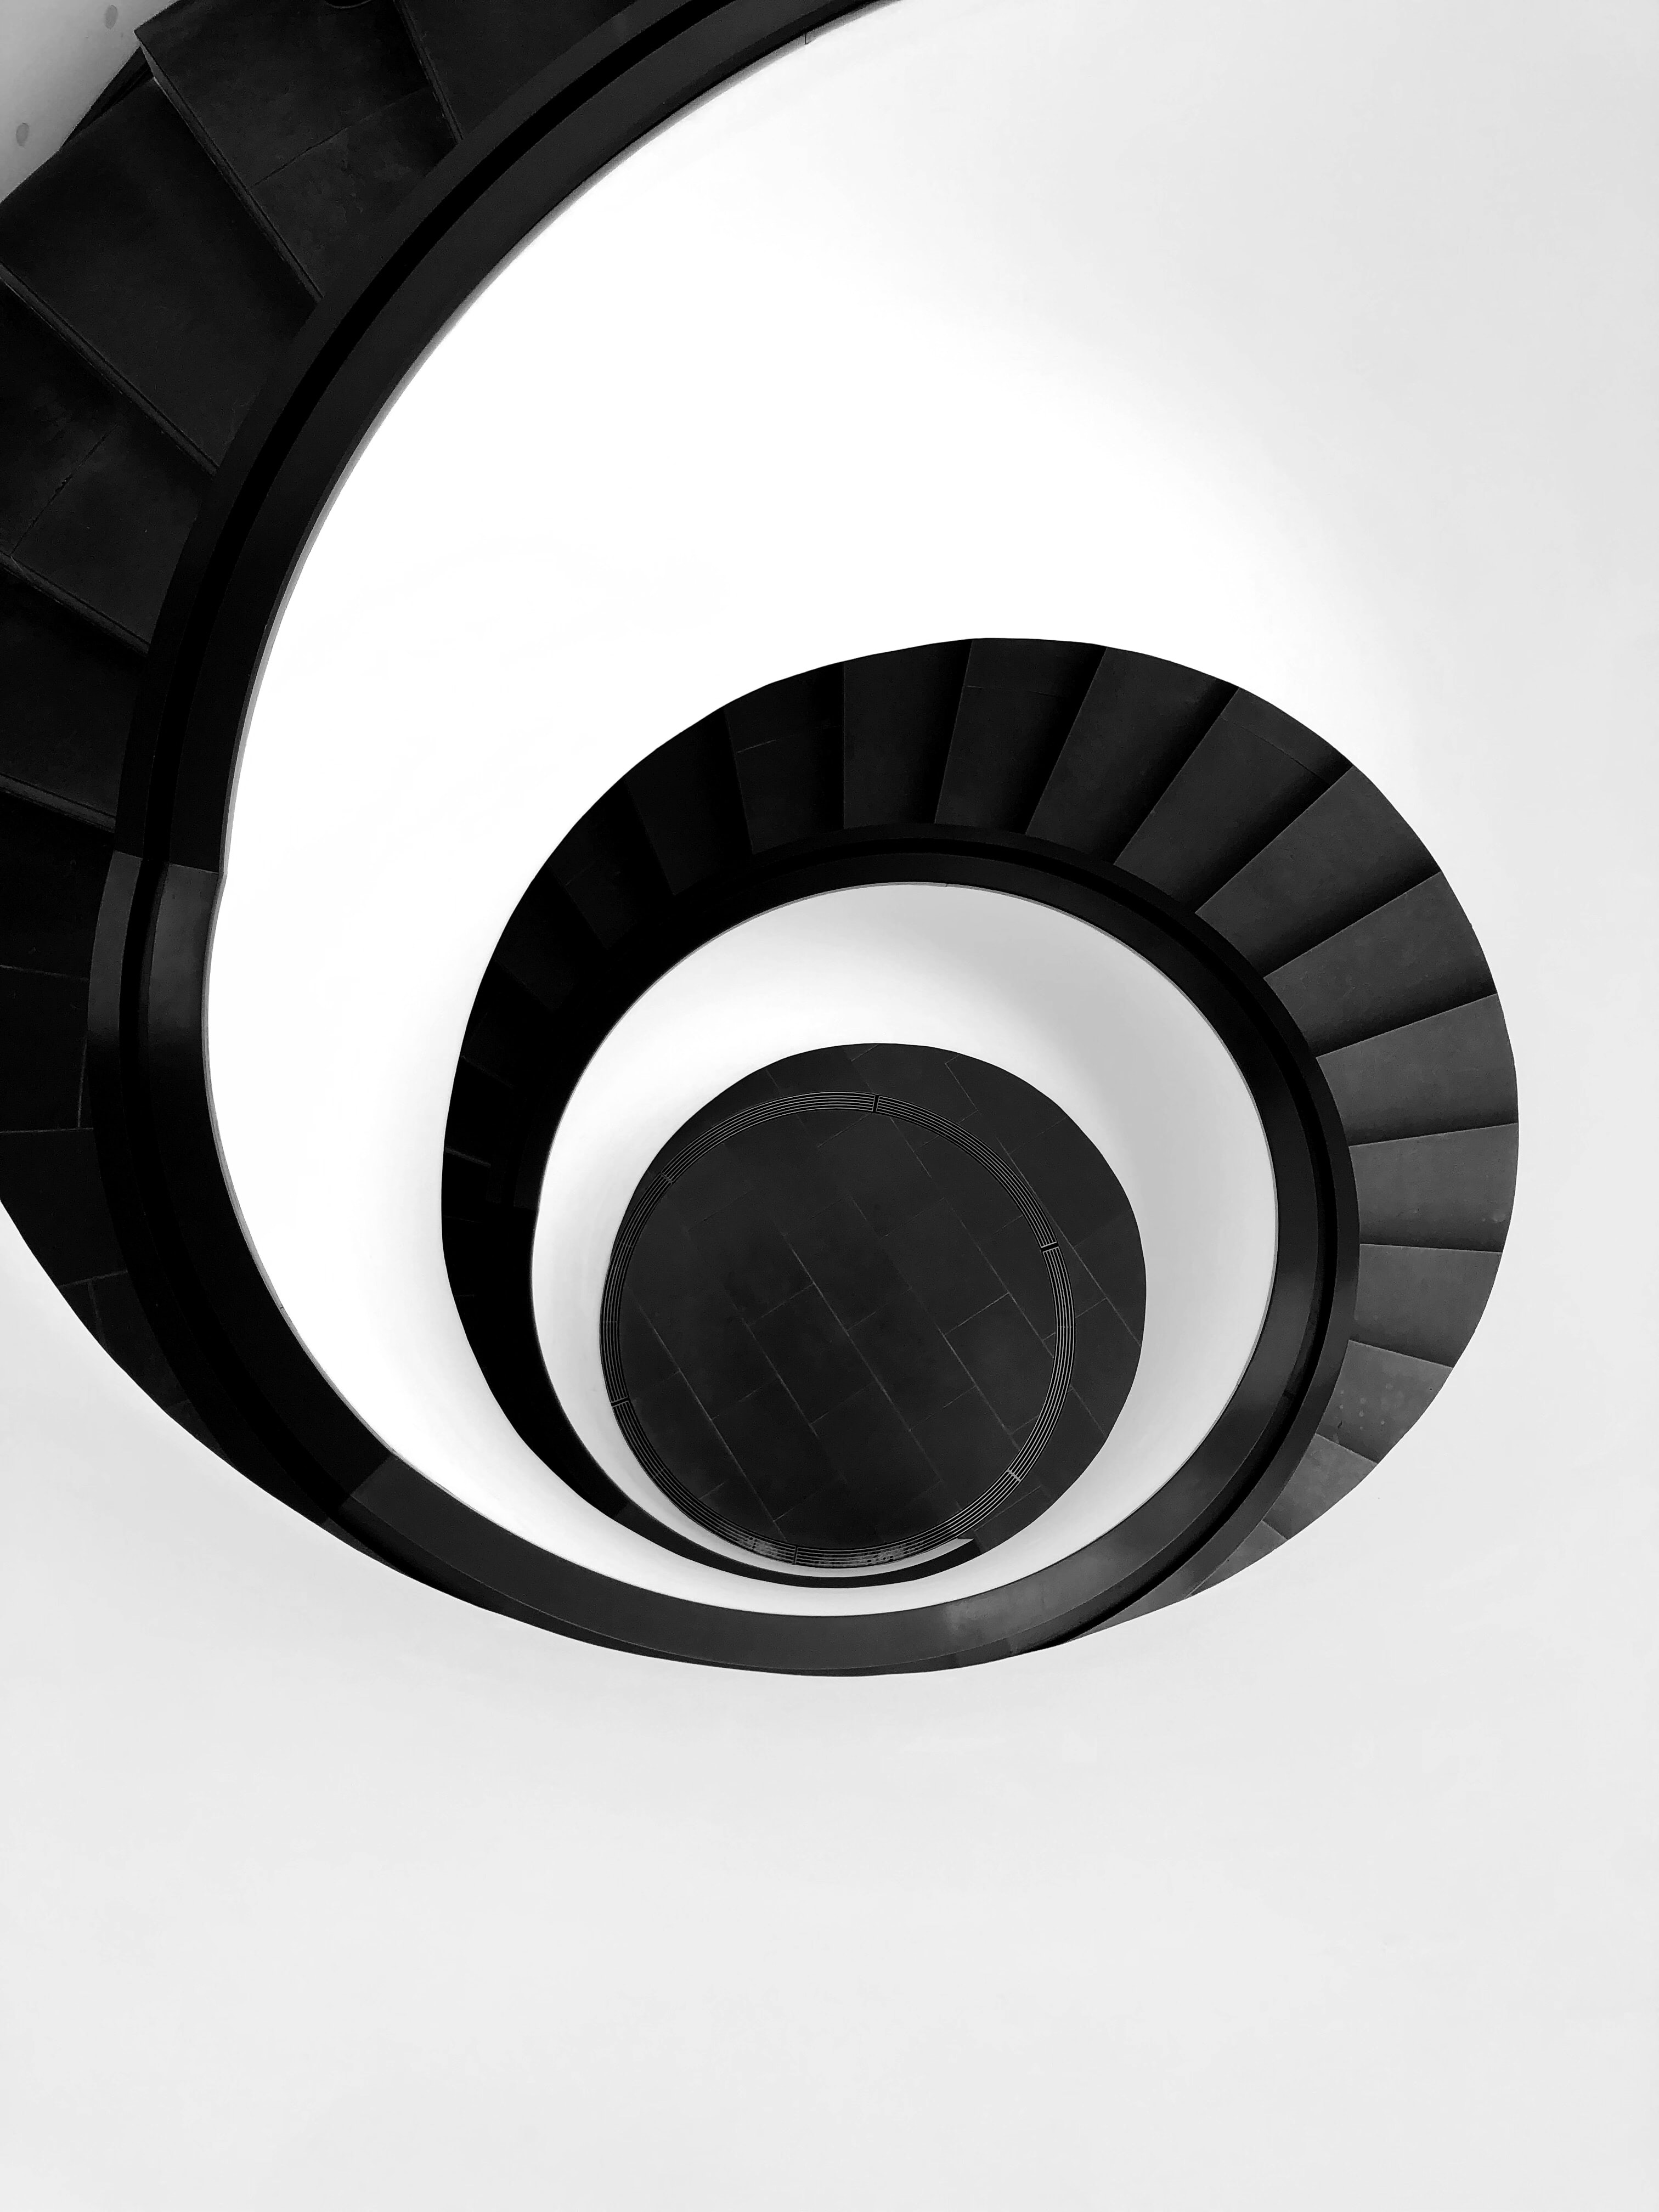
\includegraphics[width=0.4\textwidth,height=\textheight]{./img/spiral-robin-schreiner-d8OiIdAdKNA-unsplash.jpg}

}

\caption{Og så videre}

\end{figure}

\bookmarksetup{startatroot}

\hypertarget{data-frame}{%
\chapter{Data frame}\label{data-frame}}

Vi arbeider mest med datasett, og disse har en egen klasse i R, nemlig
\emph{data frame}. Jeg kommer ikke på noen god norsk oversettelse av
\emph{data frame}, så jeg bruker det engelske ordet. Dette fordi jeg på
engelsk ville skilt mellom \emph{datasets}, altså et datasett som kunne
finnes i ulike dataformater (\texttt{.sav}, \texttt{.csv},
\texttt{.xlsx}) og \emph{data frames}, altså en datastruktur i R.

\begin{Shaded}
\begin{Highlighting}[]
\CommentTok{\# En enkel data frame.}
\NormalTok{dat1 }\OtherTok{\textless{}{-}} \FunctionTok{data.frame}\NormalTok{(}
  \AttributeTok{personer =} \FunctionTok{c}\NormalTok{(}\StringTok{"Luke"}\NormalTok{, }\StringTok{"Han"}\NormalTok{, }\StringTok{"Darth"}\NormalTok{),}
  \AttributeTok{moral =} \FunctionTok{c}\NormalTok{(}\StringTok{"Bra"}\NormalTok{, }\StringTok{"Nja"}\NormalTok{, }\StringTok{"Dårlig"}\NormalTok{)}
\NormalTok{)}
\NormalTok{dat1}
\end{Highlighting}
\end{Shaded}

\begin{verbatim}
  personer  moral
1     Luke    Bra
2      Han    Nja
3    Darth Dårlig
\end{verbatim}

\begin{Shaded}
\begin{Highlighting}[]
\CommentTok{\# Vi kan lage et data frame via vektorer som er predefinerte,}
\CommentTok{\# så lenge begge har lik lengde.}
\NormalTok{dat2 }\OtherTok{\textless{}{-}} \FunctionTok{data.frame}\NormalTok{(}
  \AttributeTok{colA =}\NormalTok{ vektor1,}
  \AttributeTok{colB =}\NormalTok{ vektor2}
\NormalTok{)}
\NormalTok{dat2}
\end{Highlighting}
\end{Shaded}

\begin{verbatim}
  colA colB
1    1    A
2    2    B
3    3    C
\end{verbatim}

Det interessante med data frames er at de faktisk bare er
\textbf{lister}. Det vil si at mye av det vi veit om lister kan brukes
på data frames. Et data frame er strengt tatt bare ei liste med
vektorer. Hver vektor blir en \emph{kolonne} i data framen. Hva
representerer hver \textbf{rad}? Det er ikke gitt, men vi kan vanligvis
tenke på hver rad som en observasjon. Når vi prater om \emph{tidy data}
vil dette bli utdypa.

\begin{Shaded}
\begin{Highlighting}[]
\CommentTok{\# Sjekk ut første element av dat1}
\NormalTok{dat1[}\DecValTok{1}\NormalTok{]}
\end{Highlighting}
\end{Shaded}

\begin{verbatim}
  personer
1     Luke
2      Han
3    Darth
\end{verbatim}

Det er noen begrensninger eller krav ved datasett: hver kolonne må ha
lik lengde. Hvis ikke får du feilmelding.

\begin{Shaded}
\begin{Highlighting}[]
\NormalTok{dat3 }\OtherTok{\textless{}{-}} \FunctionTok{data.frame}\NormalTok{(}
  \AttributeTok{colA =} \FunctionTok{c}\NormalTok{(}\DecValTok{1}\NormalTok{, }\DecValTok{2}\NormalTok{, }\DecValTok{3}\NormalTok{, }\DecValTok{4}\NormalTok{),}
  \AttributeTok{colB =} \FunctionTok{c}\NormalTok{(}\DecValTok{5}\NormalTok{, }\DecValTok{6}\NormalTok{, }\DecValTok{7}\NormalTok{)}
\NormalTok{)}
\end{Highlighting}
\end{Shaded}

\begin{verbatim}
Error in data.frame(colA = c(1, 2, 3, 4), colB = c(5, 6, 7)): arguments imply differing number of rows: 4, 3
\end{verbatim}

R er snill og gir oss tydelig beskjed om hva som er galt i feilmeldinga.

En ting som er fint med alle disse R-pakkene, er at de ofte inkluderer
datasett som vi kan bruke for å illustrere pakkens funksjoner. Disse
datasetta ligger tilgjengelig på samme måte som funksjonene: man bare
skriver navnet dens for å påkalle den. La oss hente et datasett som
kommer fra \texttt{dplyr} (som er en del av \texttt{tidyverse}).

\begin{Shaded}
\begin{Highlighting}[]
\NormalTok{starwars}
\end{Highlighting}
\end{Shaded}

\begin{verbatim}
# A tibble: 87 x 14
   name        height  mass hair_~1 skin_~2 eye_c~3 birth~4 sex   gender homew~5
   <chr>        <int> <dbl> <chr>   <chr>   <chr>     <dbl> <chr> <chr>  <chr>  
 1 Luke Skywa~    172    77 blond   fair    blue       19   male  mascu~ Tatooi~
 2 C-3PO          167    75 <NA>    gold    yellow    112   none  mascu~ Tatooi~
 3 R2-D2           96    32 <NA>    white,~ red        33   none  mascu~ Naboo  
 4 Darth Vader    202   136 none    white   yellow     41.9 male  mascu~ Tatooi~
 5 Leia Organa    150    49 brown   light   brown      19   fema~ femin~ Aldera~
 6 Owen Lars      178   120 brown,~ light   blue       52   male  mascu~ Tatooi~
 7 Beru White~    165    75 brown   light   blue       47   fema~ femin~ Tatooi~
 8 R5-D4           97    32 <NA>    white,~ red        NA   none  mascu~ Tatooi~
 9 Biggs Dark~    183    84 black   light   brown      24   male  mascu~ Tatooi~
10 Obi-Wan Ke~    182    77 auburn~ fair    blue-g~    57   male  mascu~ Stewjon
# ... with 77 more rows, 4 more variables: species <chr>, films <list>,
#   vehicles <list>, starships <list>, and abbreviated variable names
#   1: hair_color, 2: skin_color, 3: eye_color, 4: birth_year, 5: homeworld
\end{verbatim}

Det kan føles rart å jobbe med data som vi ikke veit hvor ligger. Så jeg
kan plassere det explisitt i \textbf{miljøet} vårt (\emph{environment}),
ved å \emph{assigne} det.

\begin{Shaded}
\begin{Highlighting}[]
\CommentTok{\# Hvis du kjører denne koden vil du se at et objekt ved navn \textasciigrave{}starwars\textasciigrave{} dukker }
\CommentTok{\# opp i det globale miljøet i vinduet til høyre.}
\NormalTok{starwars }\OtherTok{\textless{}{-}}\NormalTok{ starwars}
\end{Highlighting}
\end{Shaded}

La oss bruke dette datasettet for å vise noen flere egenskaper ved R.
Men vent, er dette et \emph{data frame}?

\begin{Shaded}
\begin{Highlighting}[]
\NormalTok{starwars }\SpecialCharTok{\%\textgreater{}\%} \FunctionTok{class}\NormalTok{()}
\end{Highlighting}
\end{Shaded}

\begin{verbatim}
[1] "tbl_df"     "tbl"        "data.frame"
\end{verbatim}

\hypertarget{tibble}{%
\subsection{Tibble}\label{tibble}}

Som vi ser av sjekken over, har starwars tre klasser, hvor én av dem er
en \texttt{data.frame}. Til sammenlikning har de data framene vi lagde
tidligere bare én klasse:

\begin{Shaded}
\begin{Highlighting}[]
\NormalTok{dat1 }\SpecialCharTok{\%\textgreater{}\%} \FunctionTok{class}\NormalTok{()}
\end{Highlighting}
\end{Shaded}

\begin{verbatim}
[1] "data.frame"
\end{verbatim}

Så hva er en \texttt{tibble}? Kort fortalt er en tibble en forbedra
versjon av et data frame. Tibbles kommer fra pakka \texttt{tibble} som,
du gjetta riktig, er en del av \texttt{tidyverse}. En fordel med tibbles
er at de \emph{printer bedre til konsollen}. Spesielt store datasett
(vår spesialitet) blir mer leselig i tibbles. Når vi arbeider med
\texttt{tidyverse} vil mange av data framene våre bli til tibbles via
funksjonene deres. Vi trenger altså sjelden tenke mye på dette. Tibbles
arver også klassen \texttt{data.frame} som vi så over, så de fleste
funksjoner som ikke har hørt om tibbles vil også funke på dem. Flere
fordeler forklares i
\href{https://tibble.tidyverse.org/}{dokumentasjonen til pakka}.

For å oppsummere: du trenger sjelden bry deg om du jobber med tibbles
eller data frames. Jeg nevner det her fordi du kanskje vil lure på
hvorfor vi noen får \texttt{tibble}-objekter.

\hypertarget{tilbake-til-elementer}{%
\section{Tilbake til elementer}\label{tilbake-til-elementer}}

Nå som vi har tilgang til et større datasett kan vi utforske litt mer
hvordan vi arbeider med, nettopp, større datasett. Datasettet
\texttt{starwars} inneholder informasjon om dokumentarserien \emph{Star
Wars}, som omhandla livet i gamle dager, i en galakse langt, langt vekk.

\begin{Shaded}
\begin{Highlighting}[]
\NormalTok{starwars}
\end{Highlighting}
\end{Shaded}

\begin{verbatim}
# A tibble: 87 x 14
   name        height  mass hair_~1 skin_~2 eye_c~3 birth~4 sex   gender homew~5
   <chr>        <int> <dbl> <chr>   <chr>   <chr>     <dbl> <chr> <chr>  <chr>  
 1 Luke Skywa~    172    77 blond   fair    blue       19   male  mascu~ Tatooi~
 2 C-3PO          167    75 <NA>    gold    yellow    112   none  mascu~ Tatooi~
 3 R2-D2           96    32 <NA>    white,~ red        33   none  mascu~ Naboo  
 4 Darth Vader    202   136 none    white   yellow     41.9 male  mascu~ Tatooi~
 5 Leia Organa    150    49 brown   light   brown      19   fema~ femin~ Aldera~
 6 Owen Lars      178   120 brown,~ light   blue       52   male  mascu~ Tatooi~
 7 Beru White~    165    75 brown   light   blue       47   fema~ femin~ Tatooi~
 8 R5-D4           97    32 <NA>    white,~ red        NA   none  mascu~ Tatooi~
 9 Biggs Dark~    183    84 black   light   brown      24   male  mascu~ Tatooi~
10 Obi-Wan Ke~    182    77 auburn~ fair    blue-g~    57   male  mascu~ Stewjon
# ... with 77 more rows, 4 more variables: species <chr>, films <list>,
#   vehicles <list>, starships <list>, and abbreviated variable names
#   1: hair_color, 2: skin_color, 3: eye_color, 4: birth_year, 5: homeworld
\end{verbatim}

På tide å utforske. Vi kan henvise til spesifikke celler via x- og
y-koordinater.

\begin{Shaded}
\begin{Highlighting}[]
\CommentTok{\# Vi kan finne en nøyaktig celle ved å henvise til x{-} og y{-}koordinatene}
\NormalTok{starwars[}\DecValTok{2}\NormalTok{, }\DecValTok{1}\NormalTok{]}
\end{Highlighting}
\end{Shaded}

\begin{verbatim}
# A tibble: 1 x 1
  name 
  <chr>
1 C-3PO
\end{verbatim}

\begin{Shaded}
\begin{Highlighting}[]
\NormalTok{starwars[}\DecValTok{5}\NormalTok{, }\DecValTok{4}\NormalTok{]}
\end{Highlighting}
\end{Shaded}

\begin{verbatim}
# A tibble: 1 x 1
  hair_color
  <chr>     
1 brown     
\end{verbatim}

\begin{Shaded}
\begin{Highlighting}[]
\CommentTok{\# Vi kan få tak i en serie med elementer via \textasciigrave{}:\textasciigrave{}}
\NormalTok{starwars[}\DecValTok{1}\SpecialCharTok{:}\DecValTok{3}\NormalTok{]}
\end{Highlighting}
\end{Shaded}

\begin{verbatim}
# A tibble: 87 x 3
   name               height  mass
   <chr>               <int> <dbl>
 1 Luke Skywalker        172    77
 2 C-3PO                 167    75
 3 R2-D2                  96    32
 4 Darth Vader           202   136
 5 Leia Organa           150    49
 6 Owen Lars             178   120
 7 Beru Whitesun lars    165    75
 8 R5-D4                  97    32
 9 Biggs Darklighter     183    84
10 Obi-Wan Kenobi        182    77
# ... with 77 more rows
\end{verbatim}

\begin{Shaded}
\begin{Highlighting}[]
\CommentTok{\# Vi kan gjøre et utvalg av celler ved å definere både x og y som en serie}
\NormalTok{starwars[}\DecValTok{2}\SpecialCharTok{:}\DecValTok{5}\NormalTok{, }\DecValTok{6}\SpecialCharTok{:}\DecValTok{9}\NormalTok{]}
\end{Highlighting}
\end{Shaded}

\begin{verbatim}
# A tibble: 4 x 4
  eye_color birth_year sex    gender   
  <chr>          <dbl> <chr>  <chr>    
1 yellow         112   none   masculine
2 red             33   none   masculine
3 yellow          41.9 male   masculine
4 brown           19   female feminine 
\end{verbatim}

Det er upraktisk å skulle huske indekser til alt. Heldigvis kan vi
henvise til kolonner dersom de er navngitt, slik som her:

\begin{Shaded}
\begin{Highlighting}[]
\NormalTok{starwars[}\StringTok{"eye\_color"}\NormalTok{]}
\end{Highlighting}
\end{Shaded}

\begin{verbatim}
# A tibble: 87 x 1
   eye_color
   <chr>    
 1 blue     
 2 yellow   
 3 red      
 4 yellow   
 5 brown    
 6 blue     
 7 blue     
 8 red      
 9 brown    
10 blue-gray
# ... with 77 more rows
\end{verbatim}

\begin{Shaded}
\begin{Highlighting}[]
\CommentTok{\# En nyttig funksjon for å finne navna til alle kolonnene (variablene) er:}
\FunctionTok{colnames}\NormalTok{(starwars)}
\end{Highlighting}
\end{Shaded}

\begin{verbatim}
 [1] "name"       "height"     "mass"       "hair_color" "skin_color"
 [6] "eye_color"  "birth_year" "sex"        "gender"     "homeworld" 
[11] "species"    "films"      "vehicles"   "starships" 
\end{verbatim}

\begin{Shaded}
\begin{Highlighting}[]
\NormalTok{starwars[}\StringTok{"species"}\NormalTok{]}
\end{Highlighting}
\end{Shaded}

\begin{verbatim}
# A tibble: 87 x 1
   species
   <chr>  
 1 Human  
 2 Droid  
 3 Droid  
 4 Human  
 5 Human  
 6 Human  
 7 Human  
 8 Droid  
 9 Human  
10 Human  
# ... with 77 more rows
\end{verbatim}

Et alterntiv til klammeparantesen er å bruke operatoren `\$´.

\begin{Shaded}
\begin{Highlighting}[]
\CommentTok{\# Her trenger man ikke hermetegn, med mindre kolonna har mellomrom.}
\NormalTok{starwars}\SpecialCharTok{$}\NormalTok{name}
\end{Highlighting}
\end{Shaded}

\begin{verbatim}
 [1] "Luke Skywalker"        "C-3PO"                 "R2-D2"                
 [4] "Darth Vader"           "Leia Organa"           "Owen Lars"            
 [7] "Beru Whitesun lars"    "R5-D4"                 "Biggs Darklighter"    
[10] "Obi-Wan Kenobi"        "Anakin Skywalker"      "Wilhuff Tarkin"       
[13] "Chewbacca"             "Han Solo"              "Greedo"               
[16] "Jabba Desilijic Tiure" "Wedge Antilles"        "Jek Tono Porkins"     
[19] "Yoda"                  "Palpatine"             "Boba Fett"            
[22] "IG-88"                 "Bossk"                 "Lando Calrissian"     
[25] "Lobot"                 "Ackbar"                "Mon Mothma"           
[28] "Arvel Crynyd"          "Wicket Systri Warrick" "Nien Nunb"            
[31] "Qui-Gon Jinn"          "Nute Gunray"           "Finis Valorum"        
[34] "Jar Jar Binks"         "Roos Tarpals"          "Rugor Nass"           
[37] "Ric Olié"              "Watto"                 "Sebulba"              
[40] "Quarsh Panaka"         "Shmi Skywalker"        "Darth Maul"           
[43] "Bib Fortuna"           "Ayla Secura"           "Dud Bolt"             
[46] "Gasgano"               "Ben Quadinaros"        "Mace Windu"           
[49] "Ki-Adi-Mundi"          "Kit Fisto"             "Eeth Koth"            
[52] "Adi Gallia"            "Saesee Tiin"           "Yarael Poof"          
[55] "Plo Koon"              "Mas Amedda"            "Gregar Typho"         
[58] "Cordé"                 "Cliegg Lars"           "Poggle the Lesser"    
[61] "Luminara Unduli"       "Barriss Offee"         "Dormé"                
[64] "Dooku"                 "Bail Prestor Organa"   "Jango Fett"           
[67] "Zam Wesell"            "Dexter Jettster"       "Lama Su"              
[70] "Taun We"               "Jocasta Nu"            "Ratts Tyerell"        
[73] "R4-P17"                "Wat Tambor"            "San Hill"             
[76] "Shaak Ti"              "Grievous"              "Tarfful"              
[79] "Raymus Antilles"       "Sly Moore"             "Tion Medon"           
[82] "Finn"                  "Rey"                   "Poe Dameron"          
[85] "BB8"                   "Captain Phasma"        "Padmé Amidala"        
\end{verbatim}

\begin{Shaded}
\begin{Highlighting}[]
\NormalTok{starwars}\SpecialCharTok{$}\StringTok{"name"}
\end{Highlighting}
\end{Shaded}

\begin{verbatim}
 [1] "Luke Skywalker"        "C-3PO"                 "R2-D2"                
 [4] "Darth Vader"           "Leia Organa"           "Owen Lars"            
 [7] "Beru Whitesun lars"    "R5-D4"                 "Biggs Darklighter"    
[10] "Obi-Wan Kenobi"        "Anakin Skywalker"      "Wilhuff Tarkin"       
[13] "Chewbacca"             "Han Solo"              "Greedo"               
[16] "Jabba Desilijic Tiure" "Wedge Antilles"        "Jek Tono Porkins"     
[19] "Yoda"                  "Palpatine"             "Boba Fett"            
[22] "IG-88"                 "Bossk"                 "Lando Calrissian"     
[25] "Lobot"                 "Ackbar"                "Mon Mothma"           
[28] "Arvel Crynyd"          "Wicket Systri Warrick" "Nien Nunb"            
[31] "Qui-Gon Jinn"          "Nute Gunray"           "Finis Valorum"        
[34] "Jar Jar Binks"         "Roos Tarpals"          "Rugor Nass"           
[37] "Ric Olié"              "Watto"                 "Sebulba"              
[40] "Quarsh Panaka"         "Shmi Skywalker"        "Darth Maul"           
[43] "Bib Fortuna"           "Ayla Secura"           "Dud Bolt"             
[46] "Gasgano"               "Ben Quadinaros"        "Mace Windu"           
[49] "Ki-Adi-Mundi"          "Kit Fisto"             "Eeth Koth"            
[52] "Adi Gallia"            "Saesee Tiin"           "Yarael Poof"          
[55] "Plo Koon"              "Mas Amedda"            "Gregar Typho"         
[58] "Cordé"                 "Cliegg Lars"           "Poggle the Lesser"    
[61] "Luminara Unduli"       "Barriss Offee"         "Dormé"                
[64] "Dooku"                 "Bail Prestor Organa"   "Jango Fett"           
[67] "Zam Wesell"            "Dexter Jettster"       "Lama Su"              
[70] "Taun We"               "Jocasta Nu"            "Ratts Tyerell"        
[73] "R4-P17"                "Wat Tambor"            "San Hill"             
[76] "Shaak Ti"              "Grievous"              "Tarfful"              
[79] "Raymus Antilles"       "Sly Moore"             "Tion Medon"           
[82] "Finn"                  "Rey"                   "Poe Dameron"          
[85] "BB8"                   "Captain Phasma"        "Padmé Amidala"        
\end{verbatim}

Som du begynner å skjønne er det flere veier til Rom. Klammeparantesen
og \texttt{\$} har tildels overlappende funksjoner. De har likevel sine
unike bruksområder. De vil vi lære å anerkjenne etter hvert som vi
arbeider med dem. En nyttig ting med \texttt{{[}{]}} er at vi kan bruke
det som et enkelt filter.

\begin{Shaded}
\begin{Highlighting}[]
\CommentTok{\# Velg kun de karakterene som er menneske}
\NormalTok{starwars[starwars}\SpecialCharTok{$}\NormalTok{species }\SpecialCharTok{==} \StringTok{"Human"}\NormalTok{, ]}
\end{Highlighting}
\end{Shaded}

\begin{verbatim}
# A tibble: 39 x 14
   name        height  mass hair_~1 skin_~2 eye_c~3 birth~4 sex   gender homew~5
   <chr>        <int> <dbl> <chr>   <chr>   <chr>     <dbl> <chr> <chr>  <chr>  
 1 Luke Skywa~    172    77 blond   fair    blue       19   male  mascu~ Tatooi~
 2 Darth Vader    202   136 none    white   yellow     41.9 male  mascu~ Tatooi~
 3 Leia Organa    150    49 brown   light   brown      19   fema~ femin~ Aldera~
 4 Owen Lars      178   120 brown,~ light   blue       52   male  mascu~ Tatooi~
 5 Beru White~    165    75 brown   light   blue       47   fema~ femin~ Tatooi~
 6 Biggs Dark~    183    84 black   light   brown      24   male  mascu~ Tatooi~
 7 Obi-Wan Ke~    182    77 auburn~ fair    blue-g~    57   male  mascu~ Stewjon
 8 Anakin Sky~    188    84 blond   fair    blue       41.9 male  mascu~ Tatooi~
 9 Wilhuff Ta~    180    NA auburn~ fair    blue       64   male  mascu~ Eriadu 
10 Han Solo       180    80 brown   fair    brown      29   male  mascu~ Corell~
# ... with 29 more rows, 4 more variables: species <chr>, films <list>,
#   vehicles <list>, starships <list>, and abbreviated variable names
#   1: hair_color, 2: skin_color, 3: eye_color, 4: birth_year, 5: homeworld
\end{verbatim}

Dette er noe knotete: Du må gjengi datasettnavnet inni klamma, og du må
huske på kommaet for å implisitt velge alle rader. Dessuten vil du bare
få treff på nøyaktig det samme. Hvis noen har en \texttt{species} som er
skrevet f.eks. \texttt{human} eller \texttt{human/alien} vil vi ikke få
treff. Hvis det bare hadde fantes en smartere implementering av dette
filteret \ldots{}

Og det gjør det! I, nettopp, \texttt{tidyverse}!

\includegraphics[width=0.3\textwidth,height=\textheight]{./img/tidyverse-logo.png}

På tampen, noen nyttige digresjoner.

\hypertarget{digresjoner}{%
\section{Digresjoner}\label{digresjoner}}

\hypertarget{sec-navngitt-vektor}{%
\subsection{Navngitte lister/vektorer}\label{sec-navngitt-vektor}}

Vi returnerer til lister og vektorer. Tenk på de vi lagde tidligere:

\begin{Shaded}
\begin{Highlighting}[]
\NormalTok{vektor1}
\end{Highlighting}
\end{Shaded}

\begin{verbatim}
[1] 1 2 3
\end{verbatim}

\begin{Shaded}
\begin{Highlighting}[]
\NormalTok{liste1}
\end{Highlighting}
\end{Shaded}

\begin{verbatim}
[[1]]
[1] 1

[[2]]
[1] "B"

[[3]]
[1] 3

[[4]]
[1] "D"

[[5]]
[1] 5
\end{verbatim}

De er enkle. Kan vi gjøre dem \ldots{} mer komplisert? Så klart. Noe som
ofte vil være nyttig for oss er det å bruke \textbf{navngitte vektorer
eller lister} (\emph{named vector/named list}). Hva er det? Det er en
vektor eller liste hvor \emph{hvert element har et navn}. La oss se noen
eksempler. (Jeg viser bare for vektorer, men det samme gjelder for
lister.)

\begin{Shaded}
\begin{Highlighting}[]
\NormalTok{navngitt\_vektor }\OtherTok{\textless{}{-}} \FunctionTok{c}\NormalTok{(}\StringTok{"navn"} \OtherTok{=} \StringTok{"Arnold"}\NormalTok{,}
                     \StringTok{"hilsen"} \OtherTok{=} \StringTok{"hey"}\NormalTok{,}
                     \StringTok{"venn"} \OtherTok{=} \StringTok{"Gerald"}\NormalTok{)}

\CommentTok{\# Nå har hvert element i vektoren et navn}
\NormalTok{navngitt\_vektor}
\end{Highlighting}
\end{Shaded}

\begin{verbatim}
    navn   hilsen     venn 
"Arnold"    "hey" "Gerald" 
\end{verbatim}

\begin{Shaded}
\begin{Highlighting}[]
\CommentTok{\# Sammenlikn med den tidligere, navnløse vektoren. }
\NormalTok{vektor2}
\end{Highlighting}
\end{Shaded}

\begin{verbatim}
[1] "A" "B" "C"
\end{verbatim}

\begin{Shaded}
\begin{Highlighting}[]
\CommentTok{\# Vi kan også bruke funksjonen \textasciigrave{}setNames()\textasciigrave{} til å gi navn. Nyttig hvis vi har}
\CommentTok{\# navna lagra i en annen vektor/liste}
\NormalTok{navn }\OtherTok{\textless{}{-}} \FunctionTok{c}\NormalTok{(}\StringTok{"Første"}\NormalTok{, }\StringTok{"Andre"}\NormalTok{, }\StringTok{"Tredje"}\NormalTok{)}

\FunctionTok{setNames}\NormalTok{(vektor2, navn)}
\end{Highlighting}
\end{Shaded}

\begin{verbatim}
Første  Andre Tredje 
   "A"    "B"    "C" 
\end{verbatim}

\begin{Shaded}
\begin{Highlighting}[]
\CommentTok{\# Men {-}{-}{-} hvor har navna våre blitt av??}
\NormalTok{vektor2}
\end{Highlighting}
\end{Shaded}

\begin{verbatim}
[1] "A" "B" "C"
\end{verbatim}

\begin{Shaded}
\begin{Highlighting}[]
\CommentTok{\# Vi må huske å bruke *assignment* for å large det vi gjør}
\NormalTok{vektor2 }\OtherTok{\textless{}{-}} \FunctionTok{setNames}\NormalTok{(vektor2, navn)}
\NormalTok{vektor2}
\end{Highlighting}
\end{Shaded}

\begin{verbatim}
Første  Andre Tredje 
   "A"    "B"    "C" 
\end{verbatim}

Hvorfor er det nyttig? Navngitte vektorer og lister er nyttig fordi det
er mange funskjoner i spesielt \texttt{tidyverse} som nyttiggjør seg av
dem. Når man for eksempel bruker \texttt{rename()} til å endre navn på
variabler kan man sende en navngitt vektor for å endre mange navn på en
gang. Dette gjør at vi mer programmatisk kan endre navn istedenfor å
skrive hvert ledd. Når vi har mange ledd, slik som i navn på plansoner
og kommunenummer, blir dette svært nyttig.

Forresten, her er en ting jeg ofte brenner meg på: Når du bruker
\texttt{setNames()} kommer elementnavna \emph{etter} elementene. Når du
navngir elementene mens du lager vektoren/lista, kommer elemtnnavna
\emph{først}. Du ser det i eksemplene over.

\hypertarget{assignment-og--}{%
\subsection{\texorpdfstring{Assignment (\texttt{=} og
\texttt{\textless{}-})}{Assignment (= og \textless-)}}\label{assignment-og--}}

Kanskje dere føler dere lurt av noe jeg så tidligere.

\begin{quote}
Derfor bruker jeg alltid \texttt{\textless{}-}, og anbefaler deg det
også.
\end{quote}

Og litt lengre ned viser

\begin{Shaded}
\begin{Highlighting}[]
\CommentTok{\# En enkel data frame.}
\NormalTok{dat1 }\OtherTok{\textless{}{-}} \FunctionTok{data.frame}\NormalTok{(}
  \AttributeTok{personer =} \FunctionTok{c}\NormalTok{(}\StringTok{"Luke"}\NormalTok{, }\StringTok{"Han"}\NormalTok{, }\StringTok{"Darth"}\NormalTok{),}
  \AttributeTok{moral =} \FunctionTok{c}\NormalTok{(}\StringTok{"Bra"}\NormalTok{, }\StringTok{"Nja"}\NormalTok{, }\StringTok{"Dårlig"}\NormalTok{)}
\NormalTok{)}
\NormalTok{dat1}
\end{Highlighting}
\end{Shaded}

\begin{verbatim}
  personer  moral
1     Luke    Bra
2      Han    Nja
3    Darth Dårlig
\end{verbatim}

Men her bruker jeg jo \texttt{=} som assignment. Hva skjer?

Poenget her er at jeg bruker \texttt{=} inni funksjonens argumenter.
\texttt{data.frame()} er en funksjon, og jeg definerer her hva som skal
være kolonnene i datasettet mitt. Så bruker jeg \texttt{\textless{}-}
til å \emph{assigne} det som funksjonen \texttt{data.frame()}
returnerer. Forvirra? På generelt grunnlag kan vi si at vi bruker
\texttt{=} inni funksjoner, og \texttt{\textless{}-} utafor\footnote{Jeg
  gjorde det ikke hver dag.}.

Forresten, hvorfor prøver vi ikke bare å bruke \texttt{\textless{}-}
inni funksjonen og ser hva som skjer?

\begin{Shaded}
\begin{Highlighting}[]
\CommentTok{\# Funker ikke}
\NormalTok{dat1x }\OtherTok{\textless{}{-}} \FunctionTok{data.frame}\NormalTok{(}
\NormalTok{  personer }\OtherTok{\textless{}{-}} \FunctionTok{c}\NormalTok{(}\StringTok{"Luke"}\NormalTok{, }\StringTok{"Han"}\NormalTok{, }\StringTok{"Darth"}\NormalTok{),}
\NormalTok{  moral }\OtherTok{\textless{}{-}} \FunctionTok{c}\NormalTok{(}\StringTok{"Bra"}\NormalTok{, }\StringTok{"Nja"}\NormalTok{, }\StringTok{"Dårlig"}\NormalTok{)}
\NormalTok{)}

\NormalTok{dat1}
\end{Highlighting}
\end{Shaded}

\begin{verbatim}
  personer  moral
1     Luke    Bra
2      Han    Nja
3    Darth Dårlig
\end{verbatim}

\begin{Shaded}
\begin{Highlighting}[]
\NormalTok{dat1x}
\end{Highlighting}
\end{Shaded}

\begin{verbatim}
  personer....c..Luke....Han....Darth.. moral....c..Bra....Nja....Dårlig..
1                                  Luke                                Bra
2                                   Han                                Nja
3                                 Darth                             Dårlig
\end{verbatim}

Hvis vi sammenlikner de to datasetta ser vi at det funker \ldots{} på en
måte. Oppsettet blir likt, men vi mister navnet på kolonnene.

\bookmarksetup{startatroot}

\hypertarget{sec-import-export}{%
\chapter{Import og eksport av data}\label{sec-import-export}}

\begin{Shaded}
\begin{Highlighting}[]
\FunctionTok{library}\NormalTok{(tidyverse)}
\end{Highlighting}
\end{Shaded}

\begin{verbatim}
-- Attaching packages --------------------------------------- tidyverse 1.3.2 --
v ggplot2 3.3.6      v purrr   0.3.5 
v tibble  3.1.8      v dplyr   1.0.10
v tidyr   1.2.1      v stringr 1.4.1 
v readr   2.1.3      v forcats 0.5.2 
-- Conflicts ------------------------------------------ tidyverse_conflicts() --
x dplyr::filter() masks stats::filter()
x dplyr::lag()    masks stats::lag()
\end{verbatim}

\begin{Shaded}
\begin{Highlighting}[]
\FunctionTok{library}\NormalTok{(here)}
\end{Highlighting}
\end{Shaded}

\begin{verbatim}
here() starts at C:/Users/HK2Q/Documents/r/dokumentasjon
\end{verbatim}

Vi har en god del muligheter når det kommer til å laste inn data. Det er
bra, for dataene våre finnes i mange formater:

\begin{itemize}
\tightlist
\item
  \texttt{.csv}: et kommaseparert dokument. En tekstfil som vi kan lese
  med det blotte øye. Rader atskilles med linjeskift, kolonner med
  komma. I Norge bruker vi komma som desimalseparator, hvilket
  forkludrer \texttt{.csv}-filer. Derfor har vi ofte \texttt{.tsv}-filer
  istedenfor. Disse er tab-separerte. Noen ganger får de også
  forkortelsen \texttt{.csv}. Andre ganger bruker man semikolon
  istedenfor komma for å separere en \texttt{.csv}-fil. En
  \texttt{.csv}-fil er et vakkert monument til en ydmyk minimalisme og
  nøkternhet, og burde hvis gudene var sanne hadde dette vært det eneste
  dataformatet vi hadde trengt å bry oss om.
\item
  \texttt{.xlsx}: Microsoft Office Excels filformat. Disse filene jobber
  doble skift med å både lagre data og ``transformasjonene'' vi har
  gjort på det. De fungerer ut fra sin egen logikk. Dette gjør det noe
  utfordrende for oss å hente ut data fra dem. Hvor utfordrende det er
  kommer mye an på hvor konsekvent personen som har laga fila har vært.
  Her er vi ofre for en av Excels svakheter: den tillater deg å gjøre
  dumme ting. Excel er ikke et standard filformat. Kildekoden er
  proprietær og kan endres når som helst. Vi burde dermed ikke gjøre det
  til en vane å dele data i dette formatet. Likevel er det en
  kjensgjerning at mye data ligger lagra som Excel-filer, nettopp fordi
  Excel er mye brukt og det er lettvint.
\item
  \texttt{.xls}: Microsoft Office Excels gamle filformat. Funker likt
  som Excels nye filformat bortsett fra når det ikke gjør det. Hvis bare
  det hadde fantes et mer universelt datalagringsformat som holdt seg
  konstant over tid og sted. Akk ja.
\item
  \texttt{.sav}: SPSS' filformat.
\item
  \texttt{.dta}: Statas filformat.
\end{itemize}

La oss bli filosofiske et øyeblikk: hva er egentlig en datafil?

Det varierer ut fra hvilket filformat vi prater om. Hvis vi tenker oss
om, vil et svar kunne dreie seg om følgende punkter: Vi er interessert i
\textbf{datapunkter} lagra i celler. Vi kan identifisere cellene ut fra
hvilken \textbf{rad} og \textbf{kolonne} de står i. Det er fint å få med
\textbf{variabelnavn/kolonnenavn}.

Felles for mange av filformata på lista over er at de gjør mye mer enn
dette. Excel inneholder fargeformateringer på celler, funksjoner som
regner ut innhold i celler, og djevelens verste verk: den sammenslåtte
cella. SPSS kan gi oss filer med både en verdi og en merkelapp.

Den beskjedne \texttt{.csv}-fila gir oss kun det vi trenger og frister
oss ikke ut i uføre ved å la oss bli mer avanserte enn dette. Den holder
oss ærlig ved at vi ikke kan gjøre dumme ting som ødelegger for oss
seinere.

Når det er sagt, det er ikke alltid \texttt{.csv} strekker til. Når vi
jobber med kart-data trenger vi geoinformasjon, og da må vi si farvel
til fordel for
\href{https://r.geocompx.org/read-write.html\#data-output}{formater som}
\texttt{.gpkg}.

\begin{center}\rule{0.5\linewidth}{0.5pt}\end{center}

\hypertarget{felles-muxf8nstre}{%
\section{Felles mønstre}\label{felles-muxf8nstre}}

Importering og eksportering henger sammen, så vi kan omtale dem
samtidig. Det er større forskjell på de ulike formatene vi håndterer, så
vi organiserer oss etter dem. Imidlertid er det noen grunnleggende
mønstre vi kan diskutere felles.

De fleste importeringsfunksjoner kalles noe med \emph{read}, fordi de
leser inn filer. Dermed blir eksporteringsfunksjoner \emph{write}, fordi
de skriver filer til disken.

\hypertarget{filnavn}{%
\subsection{Filnavn}\label{filnavn}}

Vi må ofte definere et navn på fila vi skal skrive eller lese. Når vi
leser filer, vil navnet ofte bety både

\begin{enumerate}
\def\labelenumi{\arabic{enumi}.}
\tightlist
\item
  hva heter fila og
\item
  hvor ligger fila lagra
\end{enumerate}

Dette er fordi et filnavn strengt tatt inkludere hele \emph{filstien}
til fila. Den fila jeg arbeider på nå heter f.eks.
\texttt{import-export.qmd}. Den ligger på dette filområdet på
datamaskina mi: \texttt{C:/Users/HK2Q/Documents/r/dokumentasjon}. Dermed
blir det \emph{egentlige} navnet på fila:
\texttt{C:/Users/HK2Q/Documents/r/dokumentasjon/import-export.qmd}. Husk
at også filtutvidelsen (det som kommer ettter \texttt{.}) er en del av
filnavnet! Når en funksjon ber om \texttt{file} eller \texttt{path}
betyr dette ofte at de vil ha hele det fulle filnavnet inkludert filsti.

\hypertarget{sec-filkolasjon}{%
\subsection{Relative fillokasjoner}\label{sec-filkolasjon}}

Man kan alltids henvise til konkrete områder på maskina, men dette er
optimalt fordi det gjør at du aldri kan flytte noen filer igjen.
Dessuten vil ikke koden funke på en annen persons PC med mindre de har
100 \% likt oppsett på deres maskin. Derfor er det nyttig med
\textbf{relative} filstier. Når du arbeider i Rstudio (og du er ikke en
gærning som arbeider i R GUI, er du vel?) forventes det at du arbeider i
såkalte \textbf{prosjekter}. Alle mine prosjekter ligger kopiert på
\texttt{M:}-disken. Et prosjekt er en mappe med visse filer i seg,
hvorav den viktige fila er \texttt{prosjekt\_navn.Rproj}. Denne
opprettes automatisk når du lager et prosjekt via Rstudio. Det er mange
flotte ting med prosjekter, og en av dem er at alle filstier defineres
ut fra prosjektets \textbf{rotmappe}. Rotmappa er den mappa hvor
\texttt{.Rproj}-filer ligger, og der du putter alle mapper og filer
assosiert med prosjektet. Når du arbeider i prosjekter trenger du ikke
definere hele filstien til en fil, bare \emph{hvor den ligger i forhold
til rotmappa}. F.eks. har jeg for denne boka lagt alle bilder i en mappe
som heter \texttt{img}. Hvis jeg vil henvise til et bilde skrive jeg
bare \texttt{img/bilde.png}. Gjør det til en vane å bruke relative
filstier når du kan!

Det går så klart ikke alltid. Når noe ligger på f.eks.
\texttt{M:}-disken må jeg lage en full filsti. Fordelen er at
\texttt{M:} er en delt disk, så jeg kan anta at filstien vil se likt ut
for andre.

Merk at i noen tilfeller brytes antakelsen om at filstien alltid er
relativt til rotmappa. I disse tilfellene er pakka \texttt{here} svært
nyttig. Den er også nyttig på grunn av noe annet, nemlig
skråstrekproblematikken

\hypertarget{sec-slash}{%
\subsection{Skråstreker til besvær}\label{sec-slash}}

I Windows brukes denne skråstreket \texttt{\textbackslash{}} til å
indikere ei mappe. I alle UNIX-baserte operativsystemet og programmer
brukes \texttt{/}. Eksempler på sistnevnte er Ubuntu, macOS, og R. Når
vi arbeider med R på Windows skjer det dermed en del arbeid i kulissene
når vi henviser til en filplassering. Dette blir åpenbart for oss når vi
for eksempel forsøker å lime inn en filsti fra Windows explorer
(filutforskeren). R godtar ikke uten videre ``feil'' skråstrek. Det er
to løsninger på dette:

\begin{enumerate}
\def\labelenumi{\arabic{enumi}.}
\tightlist
\item
  endre skråstrekene så de går andre vei
\item
  \emph{escape} skråstrekene
\end{enumerate}

Det siste innebærer å bruke det som kalles \emph{escape characters}. En
del tegn har meninger i koden. F.eks. betyr \texttt{\#} kommentar i et
R-skript. Hvis jeg vil skrive ut emneknaggen, må jeg legge på en escape
character så R skjønner at dette tegnet skal ikke skal tolkes slik det
vanligvis tolkes. Hva er escape-tegnet? Det er nettopp
\texttt{\textbackslash{}}. For å escape \texttt{\#} skriver vi dermed
\texttt{\textbackslash{}\#}, og for å escape \texttt{\textbackslash{}}
skriver vi altså \texttt{\textbackslash{}\textbackslash{}}.

\begin{Shaded}
\begin{Highlighting}[]
\CommentTok{\# Ok}
\StringTok{"C:/Users/HK2Q/Documents/r/dokumentasjon"}

\CommentTok{\# Ikke ok}
\StringTok{"C:\textbackslash{}Users\textbackslash{}HK2Q\textbackslash{}Documents}\SpecialCharTok{\textbackslash{}r}\StringTok{\textbackslash{}dokumentasjon"}

\CommentTok{\# Ok}
\StringTok{"C:}\SpecialCharTok{\textbackslash{}\textbackslash{}}\StringTok{Users}\SpecialCharTok{\textbackslash{}\textbackslash{}}\StringTok{HK2Q}\SpecialCharTok{\textbackslash{}\textbackslash{}}\StringTok{Documents}\SpecialCharTok{\textbackslash{}\textbackslash{}}\StringTok{r}\SpecialCharTok{\textbackslash{}\textbackslash{}}\StringTok{dokumentasjon"}
\end{Highlighting}
\end{Shaded}

En kjapp måte å få skråstrekene etter å ha kopiert en filsti i Windows
er følgende

\begin{Shaded}
\begin{Highlighting}[]
\CommentTok{\# Skriver ut filsti med esaped \textasciigrave{}\textbackslash{}\textasciigrave{} til konsollen. Funksjonen leser }
\CommentTok{\# innholdet i utklippstavla og limer det inn i konsollen.}
\FunctionTok{paste0}\NormalTok{(}\FunctionTok{readClipboard}\NormalTok{())}
\end{Highlighting}
\end{Shaded}

Alt dette for å si: \texttt{here} pakka løser en del av problema våre.
Les mer om den på \href{https://github.com/jennybc/here_here}{Ode to the
here package}.

\hypertarget{sec-tegnkoding}{%
\subsection{Tegnkoding}\label{sec-tegnkoding}}

Spesielt når det kommer til norske \texttt{.csv}-filer hender det vi får
et problem med tegnkodinga (\emph{character encoding}). En full
gjennomgang blir for omfattende. Det holder å si at, igjen, dette er
hovedsaklig et Windows-problem. Ideelt sett vil vi ha alt over i unicode
(UTF-8). Noen filer er lagra i et annet format. Gjerne ISO8859-1 som er
en av standardene som gir oss skandinaviske tegn. En forkludrende faktor
er at det tidvis (og inntil ganske nylig, per 2023-03) har vært
problemer med R og/eller Rstudio når det kommer til tegnkoding. Disse
blir fiksa med tida og er kanskje allerede fiksa. Du ser problemet dukke
opp dersom du forventer å se en æ. ø eller å i outputen og istedet får
noe sånt som
\texttt{"\textbackslash{}xe6\textbackslash{}xf8\textbackslash{}xe5"},
\texttt{æøå} eller \texttt{\textless{}U+00C6\textgreater{}}. Der er
mange ulike faktorer som kan være årsak til dette problemet. En av dem
kan være at du må sette tegnkoden spesifikt når du leser en fil. I noen
av eksemplene mine vil du set at jeg har spesifisert \emph{encoding}, og
da er det derfor.

\hypertarget{tekstfiler-csv-med-familie}{%
\section{Tekstfiler (csv med
familie)}\label{tekstfiler-csv-med-familie}}

Vi kan bruke \texttt{read.csv()} fra \texttt{utils}, en av pakkene som
lastes når vi starter R. Det finnes også noen funksjoner fra
\texttt{readr}, en del av, 100 poeng til den som gjetter rett,
\texttt{tidyverse}. Herfra får vi \texttt{read\_csv()},
\texttt{read\_csv2()}, \texttt{read\_tsv()} og \texttt{read\_delim()}.
Les dokumentasjon for å finne mer informasjon om dem. Kort fortalt er
forskjellen at alle tre er implementeringer av den mer generelle
\texttt{\_delim()}. La oss skrive en fil og deretter last den inn.

\begin{Shaded}
\begin{Highlighting}[]
\CommentTok{\# Dette datasettet ligger klart når vi laster inn R.}
\NormalTok{mtcars}

\CommentTok{\# La oss lagre det som en csv{-}fil}
\NormalTok{mtcars }\SpecialCharTok{\%\textgreater{}\%} 
  \FunctionTok{write\_csv}\NormalTok{(}\AttributeTok{file =} \FunctionTok{here}\NormalTok{(}\StringTok{"data"}\NormalTok{, }\StringTok{"mtcars.csv"}\NormalTok{))}
\end{Highlighting}
\end{Shaded}

\begin{Shaded}
\begin{Highlighting}[]
\CommentTok{\# Og så laster vi den inn igjen}
\NormalTok{biler }\OtherTok{\textless{}{-}} \FunctionTok{read\_csv}\NormalTok{(}\AttributeTok{file =} \FunctionTok{here}\NormalTok{(}\StringTok{"data"}\NormalTok{, }\StringTok{"mtcars.csv"}\NormalTok{), }\AttributeTok{name\_repair =} \StringTok{"universal"}\NormalTok{)}
\end{Highlighting}
\end{Shaded}

\begin{verbatim}
Rows: 32 Columns: 11
-- Column specification --------------------------------------------------------
Delimiter: ","
dbl (11): mpg, cyl, disp, hp, drat, wt, qsec, vs, am, gear, carb

i Use `spec()` to retrieve the full column specification for this data.
i Specify the column types or set `show_col_types = FALSE` to quiet this message.
\end{verbatim}

\begin{Shaded}
\begin{Highlighting}[]
\NormalTok{biler}
\end{Highlighting}
\end{Shaded}

\begin{verbatim}
# A tibble: 32 x 11
     mpg   cyl  disp    hp  drat    wt  qsec    vs    am  gear  carb
   <dbl> <dbl> <dbl> <dbl> <dbl> <dbl> <dbl> <dbl> <dbl> <dbl> <dbl>
 1  21       6  160    110  3.9   2.62  16.5     0     1     4     4
 2  21       6  160    110  3.9   2.88  17.0     0     1     4     4
 3  22.8     4  108     93  3.85  2.32  18.6     1     1     4     1
 4  21.4     6  258    110  3.08  3.22  19.4     1     0     3     1
 5  18.7     8  360    175  3.15  3.44  17.0     0     0     3     2
 6  18.1     6  225    105  2.76  3.46  20.2     1     0     3     1
 7  14.3     8  360    245  3.21  3.57  15.8     0     0     3     4
 8  24.4     4  147.    62  3.69  3.19  20       1     0     4     2
 9  22.8     4  141.    95  3.92  3.15  22.9     1     0     4     2
10  19.2     6  168.   123  3.92  3.44  18.3     1     0     4     4
# ... with 22 more rows
\end{verbatim}

Jeg foretrekker \texttt{readr}s funksjoner fordi de har mange nyttige
alternativer slik som \texttt{name\_repair\ =\ "universal"}. Denne
passer på at navna i datasettet er på et format som R tolererer. F.eks.
at de ikke har mellomrom i seg. Veldig nyttig. Med \texttt{na\ =} kan du
fortelle R hvordan missing er lagra i fila du importerer.

\hypertarget{spss-1}{%
\section{SPSS}\label{spss-1}}

For SPSS-filer bruker vi pakka \texttt{haven}. Denne pakka er en del av
\ldots{} ja, du skjønner.

\begin{Shaded}
\begin{Highlighting}[]
\FunctionTok{library}\NormalTok{(haven)}
\CommentTok{\# Lagrer en fil som en spss{-}fil. (Jeg lagrer bare de første fire kolonnene).}
\NormalTok{starwars }\SpecialCharTok{\%\textgreater{}\%} 
  \FunctionTok{select}\NormalTok{(}\DecValTok{1}\SpecialCharTok{:}\DecValTok{4}\NormalTok{) }\SpecialCharTok{\%\textgreater{}\%} 
  \FunctionTok{write\_sav}\NormalTok{(}\FunctionTok{here}\NormalTok{(}\StringTok{"data"}\NormalTok{, }\StringTok{"starwars.sav"}\NormalTok{))}
\end{Highlighting}
\end{Shaded}

\begin{Shaded}
\begin{Highlighting}[]
\CommentTok{\# Les inn en spss{-}fil}
\NormalTok{stjernekrig }\OtherTok{\textless{}{-}} \FunctionTok{read\_sav}\NormalTok{(}\FunctionTok{here}\NormalTok{(}\StringTok{"data"}\NormalTok{, }\StringTok{"starwars.sav"}\NormalTok{), }\AttributeTok{.name\_repair =} \StringTok{"universal"}\NormalTok{)}
\NormalTok{stjernekrig }\SpecialCharTok{\%\textgreater{}\%} \FunctionTok{head}\NormalTok{()}
\end{Highlighting}
\end{Shaded}

\begin{verbatim}
# A tibble: 6 x 4
  name           height  mass hair_color   
  <chr>           <dbl> <dbl> <chr>        
1 Luke Skywalker    172    77 "blond"      
2 C-3PO             167    75 ""           
3 R2-D2              96    32 ""           
4 Darth Vader       202   136 "none"       
5 Leia Organa       150    49 "brown"      
6 Owen Lars         178   120 "brown, grey"
\end{verbatim}

Legger du merke til noe med fila over? Hva om jeg printer ut de
tilsvarende kolonner fra det opprinnelige datasettet vårt?

\begin{Shaded}
\begin{Highlighting}[]
\NormalTok{starwars }\SpecialCharTok{\%\textgreater{}\%} 
  \FunctionTok{select}\NormalTok{(}\DecValTok{1}\SpecialCharTok{:}\DecValTok{4}\NormalTok{) }\SpecialCharTok{\%\textgreater{}\%} 
  \FunctionTok{head}\NormalTok{()}
\end{Highlighting}
\end{Shaded}

\begin{verbatim}
# A tibble: 6 x 4
  name           height  mass hair_color 
  <chr>           <int> <dbl> <chr>      
1 Luke Skywalker    172    77 blond      
2 C-3PO             167    75 <NA>       
3 R2-D2              96    32 <NA>       
4 Darth Vader       202   136 none       
5 Leia Organa       150    49 brown      
6 Owen Lars         178   120 brown, grey
\end{verbatim}

Hårfarge har mista \texttt{NA}-designasjonen. Nå er de som før var
missing bare tomme. Dette kan skape hodebry for oss seinere, så det er
bra vi oppdaga det nå.

For å være helt ærlig er jeg ikke sikker på hvordan man løser dette
direkte. Feilen oppstår enten når vi eksporterer til \texttt{.sav} eller
importerer tilbake til R. Kanskje finnes det et svar i
\href{https://haven.tidyverse.org/articles/semantics.html\#tagged-missing-values}{Havens
dokumentasjon}. Imidlertid er det lett å omgå problemet i ettertid:

\begin{Shaded}
\begin{Highlighting}[]
\CommentTok{\# Lag ny versjon av hårfarge. Hvis hårfarge er tom (""), bli missing. Ellers, }
\CommentTok{\# bli det du allerede er. }
\NormalTok{stjernekrig }\OtherTok{\textless{}{-}}\NormalTok{ stjernekrig }\SpecialCharTok{\%\textgreater{}\%} 
  \FunctionTok{mutate}\NormalTok{(}
    \AttributeTok{hair\_color =} \FunctionTok{if\_else}\NormalTok{(}
\NormalTok{      hair\_color }\SpecialCharTok{==} \StringTok{""}\NormalTok{, }
      \ConstantTok{NA\_character\_}\NormalTok{, }
\NormalTok{      hair\_color)}
\NormalTok{    )}
\NormalTok{stjernekrig }\SpecialCharTok{\%\textgreater{}\%} \FunctionTok{head}\NormalTok{()}
\end{Highlighting}
\end{Shaded}

\begin{verbatim}
# A tibble: 6 x 4
  name           height  mass hair_color 
  <chr>           <dbl> <dbl> <chr>      
1 Luke Skywalker    172    77 blond      
2 C-3PO             167    75 <NA>       
3 R2-D2              96    32 <NA>       
4 Darth Vader       202   136 none       
5 Leia Organa       150    49 brown      
6 Owen Lars         178   120 brown, grey
\end{verbatim}

Hvorfor \texttt{NA\_character\_} og ikke bare \texttt{NA}?
\texttt{if\_else} forventer at alle argumentene skal være av samme
type/klasse. Derfor må til og med NA være en spesiell type NA. Siden
\emph{hair\_color} er en strengvektor, må NA være en streng-NA.

Når vi laster inn SPSS-filer vil vi ofte få med merkelappene
(\emph{labels}) derfra også, i form av attributter.
\texttt{tidyverse}-pakker talker ofte dette og viser dem når vi printer
objektene. Noen ganger har jeg opplevd, med andre pakker, at
attributtene ikke kan leses. I så fall kan man bare fjerne dem.

\hypertarget{excel-1}{%
\section{Excel}\label{excel-1}}

Jeg er unødvendig streng mot Excel fordi jeg gjerne vil ha ut en enkel
datastruktur fra Excels filer, mens Excel tillater oss kompliserte
strukturer som ikke uten videre kan puttes inn en en vanlig tabell. Som
sagt er vi her avhengig av den enkelte person som lagde Excelfila når
det kommer til hvor lett det er for oss å laste den inn. Det å være
konsekvent er viktigere enn å etterlikne en ``vanlig tabell''. Til dette
arbeidet har vi to pakker som har ulike bruksområder:

\begin{itemize}
\tightlist
\item
  \texttt{openxlsx}: \href{https://ycphs.github.io/openxlsx/}{Kilde}.
  Brukes for å skrive Excel-filer.
\item
  \texttt{readxl}: \href{https://readxl.tidyverse.org/}{Kilde}. Brukes
  for å lese Excel-filer.
\end{itemize}

\hypertarget{skrive-til-excel-openxlsx}{%
\subsection{\texorpdfstring{Skrive til Excel:
\texttt{openxlsx}}{Skrive til Excel: openxlsx}}\label{skrive-til-excel-openxlsx}}

Pakkas egen
\href{https://ycphs.github.io/openxlsx/articles/Introduction.html}{introduksjon}
er en god guide til hvordan dette funker. Sjekk den ut. I korte drag:

\begin{Shaded}
\begin{Highlighting}[]
\FunctionTok{library}\NormalTok{(openxlsx)}

\CommentTok{\# Kjapp lagring av fil}
\NormalTok{starwars }\SpecialCharTok{\%\textgreater{}\%} \FunctionTok{write.xlsx}\NormalTok{()}

\CommentTok{\# Hvis du vil ha det som en tabell }
\NormalTok{starwars }\SpecialCharTok{\%\textgreater{}\%} \FunctionTok{write.xlsx}\NormalTok{(}\AttributeTok{asTable =} \ConstantTok{TRUE}\NormalTok{)}
\end{Highlighting}
\end{Shaded}

Her ser vi forøvrig en demonstrasjon av hvordan et argument er valgfritt
fordi det er definert en default-verdi. I definisjonen av
\texttt{write.xlsx()} står det at argumentet \texttt{asTable} er satt
til \texttt{FALSE}. Dermed trenger vi ikke spesifisere dette med mindre
vi vil endre den til noe annet, slik vi gjør i siste linje.

Man kan også bygge opp en excelfil mer gradvis

\begin{Shaded}
\begin{Highlighting}[]
\FunctionTok{library}\NormalTok{(openxlsx)}

\CommentTok{\# Start med å lage et workbook{-}objekt}
\NormalTok{wb }\OtherTok{\textless{}{-}} \FunctionTok{createWorkbook}\NormalTok{()}

\CommentTok{\# Legg til (tomme) arkfaner}
\FunctionTok{addWorksheet}\NormalTok{(wb, }\AttributeTok{sheetName =} \StringTok{"Motor Trend Car Road Tests"}\NormalTok{, }\AttributeTok{gridLines =} \ConstantTok{FALSE}\NormalTok{)}
\FunctionTok{addWorksheet}\NormalTok{(wb, }\AttributeTok{sheetName =} \StringTok{"Iris"}\NormalTok{, }\AttributeTok{gridLines =} \ConstantTok{FALSE}\NormalTok{)}

\CommentTok{\# Skriv data til disse arkfanene. \textasciigrave{}mtcars\textasciigrave{} og \textasciigrave{}iris\textasciigrave{} er datasett som ligger i R.}
\FunctionTok{writeDataTable}\NormalTok{(wb, }\AttributeTok{sheet =} \DecValTok{1}\NormalTok{, }\AttributeTok{x =}\NormalTok{ mtcars, }\AttributeTok{colNames =} \ConstantTok{TRUE}\NormalTok{, }\AttributeTok{rowNames =} \ConstantTok{TRUE}\NormalTok{, }\AttributeTok{tableStyle =} \StringTok{"TableStyleLight9"}\NormalTok{)}
\FunctionTok{writeDataTable}\NormalTok{(wb, }\AttributeTok{sheet =} \DecValTok{2}\NormalTok{, iris, }\AttributeTok{startCol =} \StringTok{"K"}\NormalTok{, }\AttributeTok{startRow =} \DecValTok{2}\NormalTok{)}

\CommentTok{\# Lagre fila som excel{-}fil.}
\FunctionTok{saveWorkbook}\NormalTok{(wb, }\FunctionTok{here}\NormalTok{(}\StringTok{"data"}\NormalTok{, }\StringTok{"basics.xlsx"}\NormalTok{), }\AttributeTok{overwrite =} \ConstantTok{TRUE}\NormalTok{)}
\end{Highlighting}
\end{Shaded}

Dette lar deg spesifisere flere av de grafiske elementa i excel-fila,
blant annet.

En apropos, dersom du har mestra pipa (\texttt{\%\textgreater{}\%}): Man
kan ikke uten videre pipe sammen de forskjellige kommandoene i denne
pakka slik man kan med datasett. Dette gir feil:

\begin{Shaded}
\begin{Highlighting}[]
\CommentTok{\# Start med å lage et workbook{-}objekt}
\NormalTok{wb }\OtherTok{\textless{}{-}} \FunctionTok{createWorkbook}\NormalTok{()}

\CommentTok{\# Legg til (tomme) arkfaner}
\FunctionTok{addWorksheet}\NormalTok{(wb, }\AttributeTok{sheetName =} \StringTok{"Motor Trend Car Road Tests"}\NormalTok{, }\AttributeTok{gridLines =} \ConstantTok{FALSE}\NormalTok{) }\SpecialCharTok{\%\textgreater{}\%} 
  \FunctionTok{addWorksheet}\NormalTok{(}\AttributeTok{sheetName =} \StringTok{"Iris"}\NormalTok{, }\AttributeTok{gridLines =} \ConstantTok{FALSE}\NormalTok{)}
\end{Highlighting}
\end{Shaded}

\begin{verbatim}
Error: wb must be a Workbok
\end{verbatim}

Her ser vi altså en begrensing ved \texttt{tidyverse}: Når du bruker
pakker som ikke er en del av universet deres kan vi måtte gjøre
endringer i arbeidsflyten vår.

\hypertarget{lese-excel-filer-readxl}{%
\subsection{\texorpdfstring{Lese Excel-filer:
\texttt{readxl}}{Lese Excel-filer: readxl}}\label{lese-excel-filer-readxl}}

Denne pakka er en del av \texttt{tidyverse}, så her er det bare å stappe
pipa.

La oss ta et steg tilbake og tenke på vi må gjøre når vi leser inn
Excel-filer. Det er en del konsepter i Excel som ikke finnes eller
brukes i R:

\begin{itemize}
\tightlist
\item
  tomme rader og kolonner som rammer: Det vi ser som en tom celle i
  Excel er ikke nødvendigvis at den eksisterer. La oss ikke bli for
  filosofisk her. Pakkas tekst om
  \href{https://readxl.tidyverse.org/articles/sheet-geometry.html}{regnearkgeometri}
  forklarer dette bedre enn jeg kan.
\item
  farger som indikerer et eller annet om en rad, kolonne eller celle:
  Dette pleier jeg se bort fra. Viktig informasjon om rader kan heller
  lagres i tekstformat, i f.eks. en \texttt{.Rmd}/\texttt{.qmd}-fil.
\item
  funksjoner: i R definerer vi funksjonene og kjører dem en gang.
  Funksjonene blir liggende som objekter i miljøet/skriptet, mens
  verdiene de produserer blir putta i datasettet. I Excel blir
  funksjonen og resultatet liggende i samme celle, oppå hverandre. Når
  vi laster inn fila er vi bare interessert i sjølve resultatene av
  funksjonen heller enn funksjonen i seg sjøl.
\item
  sammenslåtte celler: Disse er spesielt vanskelig. Ifg. denne posten på
  \href{https://stackoverflow.com/questions/37509886/how-to-read-merged-excel-cells-with-r}{StackOverflow}
  kan man bruke \texttt{openxlsx} for å lese slike filer. Hvis det
  gjelder noen få celler, f.eks. i overskrifter, ville jeg vurdert å
  heller manuelt gå inn og dele dem opp igjen.
\end{itemize}

Vi kan bruke \texttt{read\_excel()} fra \texttt{readxl} til å lese inn
Excel-filer. Den lar oss definere en hel del nyttige ting. Her har jeg
limt inn funksjonen med alle argumentene, så forkalrer jeg i en
kommentar hva de gjør

\begin{Shaded}
\begin{Highlighting}[]
\FunctionTok{library}\NormalTok{(readxl)}

\FunctionTok{read\_excel}\NormalTok{(}
\NormalTok{  path, }\CommentTok{\# Filsti + navn på fila du skal lese}
  \AttributeTok{sheet =} \ConstantTok{NULL}\NormalTok{, }\CommentTok{\# Hvilke(t) regneark. Enten navn eller indeks}
  \AttributeTok{range =} \ConstantTok{NULL}\NormalTok{, }\CommentTok{\# Celler du vil lese. I Excels format, f.eks. "B3:D87"}
  \AttributeTok{col\_names =} \ConstantTok{TRUE}\NormalTok{, }\CommentTok{\# Er første linje kolonnenavn?}
  \AttributeTok{col\_types =} \ConstantTok{NULL}\NormalTok{, }\CommentTok{\# Definer hvilke klasser/typer hver kolonne skal lagres som}
  \AttributeTok{na =} \StringTok{""}\NormalTok{, }\CommentTok{\# Hvis NA er lagra som noe annet enn en tom celle, skriv det her}
  \AttributeTok{trim\_ws =} \ConstantTok{TRUE}\NormalTok{, }\CommentTok{\# Automatisk fjerning av whitespace}
  \AttributeTok{skip =} \DecValTok{0}\NormalTok{, }
  \AttributeTok{n\_max =} \ConstantTok{Inf}\NormalTok{,}
  \AttributeTok{guess\_max =} \FunctionTok{min}\NormalTok{(}\DecValTok{1000}\NormalTok{, n\_max), }\CommentTok{\# Se ned}
  \AttributeTok{progress =} \FunctionTok{readxl\_progress}\NormalTok{(),}
  \AttributeTok{.name\_repair =} \StringTok{"unique"} 
\NormalTok{)}
\end{Highlighting}
\end{Shaded}

Om \texttt{guess\_max}: Hvis du ikke definerer \texttt{col\_types} vil
funksjonen gjette på hvilken type data hver kolonne inneholder. På
generelt plan er Excel god på dette. Den sliter hvis:

\begin{enumerate}
\def\labelenumi{\arabic{enumi}.}
\tightlist
\item
  ei kolonne inneholder flere enn en type og
\item
  det er mange tomme celler i starten av ei kolonne
\end{enumerate}

Det står mer om gjettinga i
\href{https://readxl.tidyverse.org/articles/cell-and-column-types.html}{Cell
and Column Types}. Angående punkt 2: dette var et problem i
barnehagekapasitetsarbeidet. Her lasta jeg inn noen områder i ei
Excel-fil som hadde mange tomme rader før det dukka opp en verdi. I
disse tilfellene kunne jeg få feilmelding fordi funksjonen forventa en
annen type verdi enn det den fant. Løsninga blei å spesifisere
kolonnetypen med \texttt{col\_types}.

\bookmarksetup{startatroot}

\hypertarget{inspisere-data}{%
\chapter{Inspisere data}\label{inspisere-data}}

\begin{Shaded}
\begin{Highlighting}[]
\FunctionTok{library}\NormalTok{(tidyverse)}
\end{Highlighting}
\end{Shaded}

\begin{verbatim}
-- Attaching packages --------------------------------------- tidyverse 1.3.2 --
v ggplot2 3.3.6      v purrr   0.3.5 
v tibble  3.1.8      v dplyr   1.0.10
v tidyr   1.2.1      v stringr 1.4.1 
v readr   2.1.3      v forcats 0.5.2 
-- Conflicts ------------------------------------------ tidyverse_conflicts() --
x dplyr::filter() masks stats::filter()
x dplyr::lag()    masks stats::lag()
\end{verbatim}

Er du vant til å jobbe i programvare som er bygd mer rundt det grafiske
brukergrensesnittet vil du nok på dette tidspunktet føle deg noe
klaustrofobisk. Hvor er dataene mine? Hvordan ser de ut? Det er bra å
inspisere dataene sine jevnlig for å sjekke at antakelsene dine om dem
stemmer. Rett som det er kan du oppdaga at det du trodde var et levende
datasett egentlig bare er et \texttt{NULL}-objekt. Derfor bør vi kjenne
til en del ulike måter å inspisere datasetta våre.

\hypertarget{view}{%
\section{View}\label{view}}

Kommandoen \texttt{View()} gir deg det nærmeste vi kommer SPSS'
\emph{Data view}-vindu. Her kan du se rader, celler og kolonner. Merk at
kommandoen har stor forbokstav - noe som er uvanlig. Du bruker det
simpelthen slik \texttt{View(starwars)}, og et nytt vindu vil dukke opp
hvor du kan bivåne data i ro og mak. Har du store mengder data er min
erfaring at scrollinga blir litt treig, og det tar litt tid å laste inn
hvert nye skjermbilde. Hvis du er lei av å skrive, kan du også
dobbeltklikke på et \texttt{data.frame}/\texttt{tibble}-objekt i
miljø-vinduet.

\hypertarget{del-inspisering}{%
\section{Del-inspisering}\label{del-inspisering}}

Den enkleste måten å inspisere et datasett på er å bare skrive navnet i
konsollen. Da blir (et utdrag) av datasettet skrevet ut.

\begin{Shaded}
\begin{Highlighting}[]
\CommentTok{\# For å gjøre disse eksemplene tydligere legger jeg på en rad{-}ID med }
\CommentTok{\# \textasciigrave{}rowid\_to\_column()\textasciigrave{} slik at vi lettere ser hvilken rad vi ser på.}
\CommentTok{\# Datasettet har biltype som "radnavn", så vi putter disse inn i en egen}
\CommentTok{\# kolonne først med \textasciigrave{}rownames\_to\_column()\textasciigrave{}.}
\NormalTok{biler }\OtherTok{\textless{}{-}}\NormalTok{ mtcars }\SpecialCharTok{\%\textgreater{}\%} 
  \FunctionTok{rownames\_to\_column}\NormalTok{(}\StringTok{"bil"}\NormalTok{) }\SpecialCharTok{\%\textgreater{}\%} 
  \FunctionTok{rowid\_to\_column}\NormalTok{(}\StringTok{"rowid"}\NormalTok{)}

\NormalTok{biler}
\end{Highlighting}
\end{Shaded}

\begin{verbatim}
   rowid                 bil  mpg cyl  disp  hp drat    wt  qsec vs am gear
1      1           Mazda RX4 21.0   6 160.0 110 3.90 2.620 16.46  0  1    4
2      2       Mazda RX4 Wag 21.0   6 160.0 110 3.90 2.875 17.02  0  1    4
3      3          Datsun 710 22.8   4 108.0  93 3.85 2.320 18.61  1  1    4
4      4      Hornet 4 Drive 21.4   6 258.0 110 3.08 3.215 19.44  1  0    3
5      5   Hornet Sportabout 18.7   8 360.0 175 3.15 3.440 17.02  0  0    3
6      6             Valiant 18.1   6 225.0 105 2.76 3.460 20.22  1  0    3
7      7          Duster 360 14.3   8 360.0 245 3.21 3.570 15.84  0  0    3
8      8           Merc 240D 24.4   4 146.7  62 3.69 3.190 20.00  1  0    4
9      9            Merc 230 22.8   4 140.8  95 3.92 3.150 22.90  1  0    4
10    10            Merc 280 19.2   6 167.6 123 3.92 3.440 18.30  1  0    4
11    11           Merc 280C 17.8   6 167.6 123 3.92 3.440 18.90  1  0    4
12    12          Merc 450SE 16.4   8 275.8 180 3.07 4.070 17.40  0  0    3
13    13          Merc 450SL 17.3   8 275.8 180 3.07 3.730 17.60  0  0    3
14    14         Merc 450SLC 15.2   8 275.8 180 3.07 3.780 18.00  0  0    3
15    15  Cadillac Fleetwood 10.4   8 472.0 205 2.93 5.250 17.98  0  0    3
16    16 Lincoln Continental 10.4   8 460.0 215 3.00 5.424 17.82  0  0    3
17    17   Chrysler Imperial 14.7   8 440.0 230 3.23 5.345 17.42  0  0    3
18    18            Fiat 128 32.4   4  78.7  66 4.08 2.200 19.47  1  1    4
19    19         Honda Civic 30.4   4  75.7  52 4.93 1.615 18.52  1  1    4
20    20      Toyota Corolla 33.9   4  71.1  65 4.22 1.835 19.90  1  1    4
21    21       Toyota Corona 21.5   4 120.1  97 3.70 2.465 20.01  1  0    3
22    22    Dodge Challenger 15.5   8 318.0 150 2.76 3.520 16.87  0  0    3
23    23         AMC Javelin 15.2   8 304.0 150 3.15 3.435 17.30  0  0    3
24    24          Camaro Z28 13.3   8 350.0 245 3.73 3.840 15.41  0  0    3
25    25    Pontiac Firebird 19.2   8 400.0 175 3.08 3.845 17.05  0  0    3
26    26           Fiat X1-9 27.3   4  79.0  66 4.08 1.935 18.90  1  1    4
27    27       Porsche 914-2 26.0   4 120.3  91 4.43 2.140 16.70  0  1    5
28    28        Lotus Europa 30.4   4  95.1 113 3.77 1.513 16.90  1  1    5
29    29      Ford Pantera L 15.8   8 351.0 264 4.22 3.170 14.50  0  1    5
30    30        Ferrari Dino 19.7   6 145.0 175 3.62 2.770 15.50  0  1    5
31    31       Maserati Bora 15.0   8 301.0 335 3.54 3.570 14.60  0  1    5
32    32          Volvo 142E 21.4   4 121.0 109 4.11 2.780 18.60  1  1    4
   carb
1     4
2     4
3     1
4     1
5     2
6     1
7     4
8     2
9     2
10    4
11    4
12    3
13    3
14    3
15    4
16    4
17    4
18    1
19    2
20    1
21    1
22    2
23    2
24    4
25    2
26    1
27    2
28    2
29    4
30    6
31    8
32    2
\end{verbatim}

I seg sjøl greit. Men man risikerer å overse noe dersom man alltid bare
inspiserer de øverste ti radene. Da er de nyttig å se på et tilfeldig
utvalg av rader

\begin{Shaded}
\begin{Highlighting}[]
\NormalTok{biler }\SpecialCharTok{\%\textgreater{}\%} \FunctionTok{slice\_sample}\NormalTok{(}\AttributeTok{n =} \DecValTok{10}\NormalTok{)}
\end{Highlighting}
\end{Shaded}

\begin{verbatim}
   rowid                bil  mpg cyl  disp  hp drat    wt  qsec vs am gear carb
1      6            Valiant 18.1   6 225.0 105 2.76 3.460 20.22  1  0    3    1
2     32         Volvo 142E 21.4   4 121.0 109 4.11 2.780 18.60  1  1    4    2
3     25   Pontiac Firebird 19.2   8 400.0 175 3.08 3.845 17.05  0  0    3    2
4     15 Cadillac Fleetwood 10.4   8 472.0 205 2.93 5.250 17.98  0  0    3    4
5     14        Merc 450SLC 15.2   8 275.8 180 3.07 3.780 18.00  0  0    3    3
6     27      Porsche 914-2 26.0   4 120.3  91 4.43 2.140 16.70  0  1    5    2
7     26          Fiat X1-9 27.3   4  79.0  66 4.08 1.935 18.90  1  1    4    1
8     20     Toyota Corolla 33.9   4  71.1  65 4.22 1.835 19.90  1  1    4    1
9     12         Merc 450SE 16.4   8 275.8 180 3.07 4.070 17.40  0  0    3    3
10     8          Merc 240D 24.4   4 146.7  62 3.69 3.190 20.00  1  0    4    2
\end{verbatim}

Denne funksjonen er en avart av \texttt{slice()} som gir deg
\emph{spesifikke} rader. Hvis du f.eks. vil ha rad 10-20:

\begin{Shaded}
\begin{Highlighting}[]
\NormalTok{biler }\SpecialCharTok{\%\textgreater{}\%} \FunctionTok{slice}\NormalTok{(}\DecValTok{10}\SpecialCharTok{:}\DecValTok{20}\NormalTok{)}
\end{Highlighting}
\end{Shaded}

\begin{verbatim}
   rowid                 bil  mpg cyl  disp  hp drat    wt  qsec vs am gear
1     10            Merc 280 19.2   6 167.6 123 3.92 3.440 18.30  1  0    4
2     11           Merc 280C 17.8   6 167.6 123 3.92 3.440 18.90  1  0    4
3     12          Merc 450SE 16.4   8 275.8 180 3.07 4.070 17.40  0  0    3
4     13          Merc 450SL 17.3   8 275.8 180 3.07 3.730 17.60  0  0    3
5     14         Merc 450SLC 15.2   8 275.8 180 3.07 3.780 18.00  0  0    3
6     15  Cadillac Fleetwood 10.4   8 472.0 205 2.93 5.250 17.98  0  0    3
7     16 Lincoln Continental 10.4   8 460.0 215 3.00 5.424 17.82  0  0    3
8     17   Chrysler Imperial 14.7   8 440.0 230 3.23 5.345 17.42  0  0    3
9     18            Fiat 128 32.4   4  78.7  66 4.08 2.200 19.47  1  1    4
10    19         Honda Civic 30.4   4  75.7  52 4.93 1.615 18.52  1  1    4
11    20      Toyota Corolla 33.9   4  71.1  65 4.22 1.835 19.90  1  1    4
   carb
1     4
2     4
3     3
4     3
5     3
6     4
7     4
8     4
9     1
10    2
11    1
\end{verbatim}

Dette gir oss en mulighet til å se fordelen med å arbeide med tibbles:
På noen skjermer blir den forrige tabellen stygg fordi den siste kolonna
presses ned til ei ny side. (Jeg kan ikke garantere at det skjer på din
side.) Men om vi gjør om \emph{biler} (som arver
\texttt{data.fram}-klassen fra \emph{mtcars}) til en \texttt{tibble},
får den siste kolonna plass på samme linje som resten. (Jeg kan
forsåvidt heller ikke garantere at dette vil se helt likt ut på din
skjerm.) Og vi får vite kolonnetypen til hver kolonne. Stilig!

\begin{Shaded}
\begin{Highlighting}[]
\NormalTok{biler }\SpecialCharTok{\%\textgreater{}\%} 
  \FunctionTok{tibble}\NormalTok{() }\SpecialCharTok{\%\textgreater{}\%} 
  \FunctionTok{slice}\NormalTok{(}\DecValTok{10}\SpecialCharTok{:}\DecValTok{20}\NormalTok{)}
\end{Highlighting}
\end{Shaded}

\begin{verbatim}
# A tibble: 11 x 13
   rowid bil     mpg   cyl  disp    hp  drat    wt  qsec    vs    am  gear  carb
   <int> <chr> <dbl> <dbl> <dbl> <dbl> <dbl> <dbl> <dbl> <dbl> <dbl> <dbl> <dbl>
 1    10 Merc~  19.2     6 168.    123  3.92  3.44  18.3     1     0     4     4
 2    11 Merc~  17.8     6 168.    123  3.92  3.44  18.9     1     0     4     4
 3    12 Merc~  16.4     8 276.    180  3.07  4.07  17.4     0     0     3     3
 4    13 Merc~  17.3     8 276.    180  3.07  3.73  17.6     0     0     3     3
 5    14 Merc~  15.2     8 276.    180  3.07  3.78  18       0     0     3     3
 6    15 Cadi~  10.4     8 472     205  2.93  5.25  18.0     0     0     3     4
 7    16 Linc~  10.4     8 460     215  3     5.42  17.8     0     0     3     4
 8    17 Chry~  14.7     8 440     230  3.23  5.34  17.4     0     0     3     4
 9    18 Fiat~  32.4     4  78.7    66  4.08  2.2   19.5     1     1     4     1
10    19 Hond~  30.4     4  75.7    52  4.93  1.62  18.5     1     1     4     2
11    20 Toyo~  33.9     4  71.1    65  4.22  1.84  19.9     1     1     4     1
\end{verbatim}

Noen ganger er det likevel nyttig å kikke på toppen eller bunnen av et
datasett. Da kan vi bruke de komplementære funksjonene \texttt{head()}
og \texttt{tail()}.

\begin{Shaded}
\begin{Highlighting}[]
\CommentTok{\# \textasciigrave{}head()\textasciigrave{} viser toppen}
\NormalTok{biler }\SpecialCharTok{\%\textgreater{}\%} \FunctionTok{head}\NormalTok{()}
\end{Highlighting}
\end{Shaded}

\begin{verbatim}
  rowid               bil  mpg cyl disp  hp drat    wt  qsec vs am gear carb
1     1         Mazda RX4 21.0   6  160 110 3.90 2.620 16.46  0  1    4    4
2     2     Mazda RX4 Wag 21.0   6  160 110 3.90 2.875 17.02  0  1    4    4
3     3        Datsun 710 22.8   4  108  93 3.85 2.320 18.61  1  1    4    1
4     4    Hornet 4 Drive 21.4   6  258 110 3.08 3.215 19.44  1  0    3    1
5     5 Hornet Sportabout 18.7   8  360 175 3.15 3.440 17.02  0  0    3    2
6     6           Valiant 18.1   6  225 105 2.76 3.460 20.22  1  0    3    1
\end{verbatim}

\begin{Shaded}
\begin{Highlighting}[]
\CommentTok{\# \textasciigrave{}tail()\textasciigrave{} viser bunnen}
\NormalTok{biler }\SpecialCharTok{\%\textgreater{}\%} \FunctionTok{tail}\NormalTok{()}
\end{Highlighting}
\end{Shaded}

\begin{verbatim}
   rowid            bil  mpg cyl  disp  hp drat    wt qsec vs am gear carb
27    27  Porsche 914-2 26.0   4 120.3  91 4.43 2.140 16.7  0  1    5    2
28    28   Lotus Europa 30.4   4  95.1 113 3.77 1.513 16.9  1  1    5    2
29    29 Ford Pantera L 15.8   8 351.0 264 4.22 3.170 14.5  0  1    5    4
30    30   Ferrari Dino 19.7   6 145.0 175 3.62 2.770 15.5  0  1    5    6
31    31  Maserati Bora 15.0   8 301.0 335 3.54 3.570 14.6  0  1    5    8
32    32     Volvo 142E 21.4   4 121.0 109 4.11 2.780 18.6  1  1    4    2
\end{verbatim}

Disse er nyttig fordi de kan brukes på mer enn bare datasett.

\begin{Shaded}
\begin{Highlighting}[]
\CommentTok{\# Viser de siste kolonnenavna i datasettet}
\NormalTok{biler }\SpecialCharTok{\%\textgreater{}\%} 
  \FunctionTok{colnames}\NormalTok{() }\SpecialCharTok{\%\textgreater{}\%} 
  \FunctionTok{tail}\NormalTok{()}
\end{Highlighting}
\end{Shaded}

\begin{verbatim}
[1] "wt"   "qsec" "vs"   "am"   "gear" "carb"
\end{verbatim}

\begin{Shaded}
\begin{Highlighting}[]
\CommentTok{\# Lager en strengvektor på 26 elementer (bokstaver)}
\NormalTok{bokstaver }\OtherTok{\textless{}{-}}\NormalTok{ letters[}\DecValTok{1}\SpecialCharTok{:}\DecValTok{26}\NormalTok{]}

\CommentTok{\# Viser de siste bokstavene}
\NormalTok{bokstaver }\SpecialCharTok{\%\textgreater{}\%} \FunctionTok{tail}\NormalTok{()}
\end{Highlighting}
\end{Shaded}

\begin{verbatim}
[1] "u" "v" "w" "x" "y" "z"
\end{verbatim}

\hypertarget{andre-kolonner}{%
\section{Andre kolonner}\label{andre-kolonner}}

På samme måte som det er begrensende å hele tida kikke på de øverste
\emph{radene} av et datasett er det begrensende å kikke på de fremste
\emph{kolonnene}. Vi kan bruke \texttt{select()} for å velge hvilke
rader vi vil se på, eller vi kan bruke den nyttige \texttt{glimpse()}.
Greier du å gjette hvor disse funksjonene kommer fra? De kommer fra
\texttt{dplyr}!

\ldots{}

som er en del av \texttt{tidyverse}.

\hypertarget{sec-select}{%
\subsection{select}\label{sec-select}}

\texttt{select()} gir oss muligheten til å diskutere en av de
fantastiske innovasjonene i \texttt{tidyverse}: \textbf{tidy
evaluation}. Vi dykker ikke dypt i det, men det er greit å vite om
\textbf{data masking} og \textbf{tidy select}. De er diskutert mer
inngående i
\href{https://dplyr.tidyverse.org/articles/programming.html}{Programming
with Tidyverse}. \emph{Tidy select} lar oss velge en kolonne i et
datasett \emph{uten å måtte hermetegn}. Tenk på det! Neste gang du
velger en kolonne slipper du å strekke lillefingeren til den fjerne
shift-tasten og gå i spagat med langefingern til 2-tasten. Faktisk gjør
\emph{tidy select} mye mer enn dette, som vi vil se etter hvert. F.eks.
kan du velge kolonner ut fra navn, posisjon, eller \emph{type}. La oss
se noen eksempler

\begin{Shaded}
\begin{Highlighting}[]
\CommentTok{\# Slik ser starwars{-}datasettet ut. }
\NormalTok{starwars }\SpecialCharTok{\%\textgreater{}\%} \FunctionTok{head}\NormalTok{()}
\end{Highlighting}
\end{Shaded}

\begin{verbatim}
# A tibble: 6 x 14
  name         height  mass hair_~1 skin_~2 eye_c~3 birth~4 sex   gender homew~5
  <chr>         <int> <dbl> <chr>   <chr>   <chr>     <dbl> <chr> <chr>  <chr>  
1 Luke Skywal~    172    77 blond   fair    blue       19   male  mascu~ Tatooi~
2 C-3PO           167    75 <NA>    gold    yellow    112   none  mascu~ Tatooi~
3 R2-D2            96    32 <NA>    white,~ red        33   none  mascu~ Naboo  
4 Darth Vader     202   136 none    white   yellow     41.9 male  mascu~ Tatooi~
5 Leia Organa     150    49 brown   light   brown      19   fema~ femin~ Aldera~
6 Owen Lars       178   120 brown,~ light   blue       52   male  mascu~ Tatooi~
# ... with 4 more variables: species <chr>, films <list>, vehicles <list>,
#   starships <list>, and abbreviated variable names 1: hair_color,
#   2: skin_color, 3: eye_color, 4: birth_year, 5: homeworld
\end{verbatim}

\begin{Shaded}
\begin{Highlighting}[]
\CommentTok{\# Det er 14 kolonner. }
\CommentTok{\# Med mindre du har en svær skjerm kan vi ikke se alle på en gang.}
\NormalTok{starwars }\SpecialCharTok{\%\textgreater{}\%} \FunctionTok{colnames}\NormalTok{()}
\end{Highlighting}
\end{Shaded}

\begin{verbatim}
 [1] "name"       "height"     "mass"       "hair_color" "skin_color"
 [6] "eye_color"  "birth_year" "sex"        "gender"     "homeworld" 
[11] "species"    "films"      "vehicles"   "starships" 
\end{verbatim}

\begin{Shaded}
\begin{Highlighting}[]
\CommentTok{\# Vi kikker på noen spesifikke kolonner. }
\CommentTok{\# Films er ei liste, så den ser vi ikke direkte.}
\NormalTok{starwars }\SpecialCharTok{\%\textgreater{}\%} \FunctionTok{select}\NormalTok{(name, species, films)}
\end{Highlighting}
\end{Shaded}

\begin{verbatim}
# A tibble: 87 x 3
   name               species films    
   <chr>              <chr>   <list>   
 1 Luke Skywalker     Human   <chr [5]>
 2 C-3PO              Droid   <chr [6]>
 3 R2-D2              Droid   <chr [7]>
 4 Darth Vader        Human   <chr [4]>
 5 Leia Organa        Human   <chr [5]>
 6 Owen Lars          Human   <chr [3]>
 7 Beru Whitesun lars Human   <chr [3]>
 8 R5-D4              Droid   <chr [1]>
 9 Biggs Darklighter  Human   <chr [1]>
10 Obi-Wan Kenobi     Human   <chr [6]>
# ... with 77 more rows
\end{verbatim}

\begin{Shaded}
\begin{Highlighting}[]
\CommentTok{\# Vi vil ha 1, 3, 5, og 7 kolonne}
\NormalTok{starwars }\SpecialCharTok{\%\textgreater{}\%} \FunctionTok{select}\NormalTok{(}\DecValTok{1}\NormalTok{, }\DecValTok{3}\NormalTok{, }\DecValTok{5}\NormalTok{, }\DecValTok{7}\NormalTok{)}
\end{Highlighting}
\end{Shaded}

\begin{verbatim}
# A tibble: 87 x 4
   name                mass skin_color  birth_year
   <chr>              <dbl> <chr>            <dbl>
 1 Luke Skywalker        77 fair              19  
 2 C-3PO                 75 gold             112  
 3 R2-D2                 32 white, blue       33  
 4 Darth Vader          136 white             41.9
 5 Leia Organa           49 light             19  
 6 Owen Lars            120 light             52  
 7 Beru Whitesun lars    75 light             47  
 8 R5-D4                 32 white, red        NA  
 9 Biggs Darklighter     84 light             24  
10 Obi-Wan Kenobi        77 fair              57  
# ... with 77 more rows
\end{verbatim}

\begin{Shaded}
\begin{Highlighting}[]
\CommentTok{\# Alle kolonner som inneholder en viss tekststreng}
\NormalTok{starwars }\SpecialCharTok{\%\textgreater{}\%} \FunctionTok{select}\NormalTok{(}\FunctionTok{contains}\NormalTok{(}\StringTok{"color"}\NormalTok{))}
\end{Highlighting}
\end{Shaded}

\begin{verbatim}
# A tibble: 87 x 3
   hair_color    skin_color  eye_color
   <chr>         <chr>       <chr>    
 1 blond         fair        blue     
 2 <NA>          gold        yellow   
 3 <NA>          white, blue red      
 4 none          white       yellow   
 5 brown         light       brown    
 6 brown, grey   light       blue     
 7 brown         light       blue     
 8 <NA>          white, red  red      
 9 black         light       brown    
10 auburn, white fair        blue-gray
# ... with 77 more rows
\end{verbatim}

\begin{Shaded}
\begin{Highlighting}[]
\CommentTok{\# Alle kolonner som er numeriske}
\NormalTok{starwars }\SpecialCharTok{\%\textgreater{}\%} \FunctionTok{select}\NormalTok{(}\FunctionTok{where}\NormalTok{(is.numeric))}
\end{Highlighting}
\end{Shaded}

\begin{verbatim}
# A tibble: 87 x 3
   height  mass birth_year
    <int> <dbl>      <dbl>
 1    172    77       19  
 2    167    75      112  
 3     96    32       33  
 4    202   136       41.9
 5    150    49       19  
 6    178   120       52  
 7    165    75       47  
 8     97    32       NA  
 9    183    84       24  
10    182    77       57  
# ... with 77 more rows
\end{verbatim}

\hypertarget{glimpse}{%
\subsection{glimpse}\label{glimpse}}

Tilbake til det opprinnelige formålet, som bare var å ta en kjapp titt
på dataene vi har. Til dette er \texttt{glimpse()} utmerka. Den snur
rett og slett datasettet 90 grader og skriver ut kolonnenavna
\emph{nedover}. Dermed får du med flere. Du får også en oversikt over
hva hver kolonne inneholder, skjønt det er mer utydelig hva som er på
samme rad. En fordel med \texttt{glimpse()} er at den viser oss
innholdet i lister som er element av datasettet. Her ser vi f.eks.
innholdet i kolonna \emph{films} .

\begin{Shaded}
\begin{Highlighting}[]
\NormalTok{starwars }\SpecialCharTok{\%\textgreater{}\%} \FunctionTok{glimpse}\NormalTok{()}
\end{Highlighting}
\end{Shaded}

\begin{verbatim}
Rows: 87
Columns: 14
$ name       <chr> "Luke Skywalker", "C-3PO", "R2-D2", "Darth Vader", "Leia Or~
$ height     <int> 172, 167, 96, 202, 150, 178, 165, 97, 183, 182, 188, 180, 2~
$ mass       <dbl> 77.0, 75.0, 32.0, 136.0, 49.0, 120.0, 75.0, 32.0, 84.0, 77.~
$ hair_color <chr> "blond", NA, NA, "none", "brown", "brown, grey", "brown", N~
$ skin_color <chr> "fair", "gold", "white, blue", "white", "light", "light", "~
$ eye_color  <chr> "blue", "yellow", "red", "yellow", "brown", "blue", "blue",~
$ birth_year <dbl> 19.0, 112.0, 33.0, 41.9, 19.0, 52.0, 47.0, NA, 24.0, 57.0, ~
$ sex        <chr> "male", "none", "none", "male", "female", "male", "female",~
$ gender     <chr> "masculine", "masculine", "masculine", "masculine", "femini~
$ homeworld  <chr> "Tatooine", "Tatooine", "Naboo", "Tatooine", "Alderaan", "T~
$ species    <chr> "Human", "Droid", "Droid", "Human", "Human", "Human", "Huma~
$ films      <list> <"The Empire Strikes Back", "Revenge of the Sith", "Return~
$ vehicles   <list> <"Snowspeeder", "Imperial Speeder Bike">, <>, <>, <>, "Imp~
$ starships  <list> <"X-wing", "Imperial shuttle">, <>, <>, "TIE Advanced x1",~
\end{verbatim}

\hypertarget{sec-oppsummering}{%
\section{Oppsummeringer}\label{sec-oppsummering}}

Hittil har vi bare prata om måter å set utdrag av data på. Noen ganger
er det nyttig å se en \emph{oppsummering} av dataene. Detaljer som
snitt, standardavvik, minimum og maksimum-verdier, for eksempel.

\texttt{summary()} fra \texttt{base\ R} er nyttig her. Den gir enkelt og
greit en oversikt over diverse statistikk for hver numeriske variabel.

\begin{Shaded}
\begin{Highlighting}[]
\NormalTok{biler }\SpecialCharTok{\%\textgreater{}\%} \FunctionTok{summary}\NormalTok{()}
\end{Highlighting}
\end{Shaded}

\begin{verbatim}
     rowid           bil                 mpg             cyl       
 Min.   : 1.00   Length:32          Min.   :10.40   Min.   :4.000  
 1st Qu.: 8.75   Class :character   1st Qu.:15.43   1st Qu.:4.000  
 Median :16.50   Mode  :character   Median :19.20   Median :6.000  
 Mean   :16.50                      Mean   :20.09   Mean   :6.188  
 3rd Qu.:24.25                      3rd Qu.:22.80   3rd Qu.:8.000  
 Max.   :32.00                      Max.   :33.90   Max.   :8.000  
      disp             hp             drat             wt       
 Min.   : 71.1   Min.   : 52.0   Min.   :2.760   Min.   :1.513  
 1st Qu.:120.8   1st Qu.: 96.5   1st Qu.:3.080   1st Qu.:2.581  
 Median :196.3   Median :123.0   Median :3.695   Median :3.325  
 Mean   :230.7   Mean   :146.7   Mean   :3.597   Mean   :3.217  
 3rd Qu.:326.0   3rd Qu.:180.0   3rd Qu.:3.920   3rd Qu.:3.610  
 Max.   :472.0   Max.   :335.0   Max.   :4.930   Max.   :5.424  
      qsec             vs               am              gear      
 Min.   :14.50   Min.   :0.0000   Min.   :0.0000   Min.   :3.000  
 1st Qu.:16.89   1st Qu.:0.0000   1st Qu.:0.0000   1st Qu.:3.000  
 Median :17.71   Median :0.0000   Median :0.0000   Median :4.000  
 Mean   :17.85   Mean   :0.4375   Mean   :0.4062   Mean   :3.688  
 3rd Qu.:18.90   3rd Qu.:1.0000   3rd Qu.:1.0000   3rd Qu.:4.000  
 Max.   :22.90   Max.   :1.0000   Max.   :1.0000   Max.   :5.000  
      carb      
 Min.   :1.000  
 1st Qu.:2.000  
 Median :2.000  
 Mean   :2.812  
 3rd Qu.:4.000  
 Max.   :8.000  
\end{verbatim}

Vi kan også sette sammen vår eget sammendrag med \texttt{summarise} fra
\texttt{dplyr}. Her kombinerer vi det med grupperingsfunksjonen
\texttt{group\_by()}.

\begin{Shaded}
\begin{Highlighting}[]
\NormalTok{mtcars }\SpecialCharTok{\%\textgreater{}\%} 
  \FunctionTok{group\_by}\NormalTok{(cyl) }\SpecialCharTok{\%\textgreater{}\%} 
  \FunctionTok{summarise}\NormalTok{(}
    \AttributeTok{mpg\_m =} \FunctionTok{mean}\NormalTok{(mpg),}
    \AttributeTok{mpg\_sd =} \FunctionTok{sd}\NormalTok{(mpg)}
\NormalTok{  )}
\end{Highlighting}
\end{Shaded}

\begin{verbatim}
# A tibble: 3 x 3
    cyl mpg_m mpg_sd
  <dbl> <dbl>  <dbl>
1     4  26.7   4.51
2     6  19.7   1.45
3     8  15.1   2.56
\end{verbatim}

\textbf{Tips}: Jeg bruker både \texttt{summary()} og
\texttt{summarise()} ofte. Og jeg bruker nesten konsekvent den ene når
jeg egentlig mener å bruke den andre. Får du feilmelding når du arbeider
med disse funksjonene, sjekk først at du ikke egentlig mente å bruke den
andre.

\bookmarksetup{startatroot}

\hypertarget{omstrukturering-av-data-pivot}{%
\chapter{Omstrukturering av data
(pivot)}\label{omstrukturering-av-data-pivot}}

\begin{Shaded}
\begin{Highlighting}[]
\FunctionTok{library}\NormalTok{(tidyverse)}
\end{Highlighting}
\end{Shaded}

\begin{verbatim}
-- Attaching packages --------------------------------------- tidyverse 1.3.2 --
v ggplot2 3.3.6      v purrr   0.3.5 
v tibble  3.1.8      v dplyr   1.0.10
v tidyr   1.2.1      v stringr 1.4.1 
v readr   2.1.3      v forcats 0.5.2 
-- Conflicts ------------------------------------------ tidyverse_conflicts() --
x dplyr::filter() masks stats::filter()
x dplyr::lag()    masks stats::lag()
\end{verbatim}

Har vi prata om \textbf{tidy data} før? Hvis ikke er tida nå.

\hypertarget{tidy-data}{%
\section{Tidy data}\label{tidy-data}}

En grundigere introduksjon finnes hos
\href{https://tidyr.tidyverse.org/articles/tidy-data.html}{Tidyverse}.
Faktisk er det en mye bedre introduksjon enn det jeg hadde greid å
skrive. Hvis du er interessert i \emph{hvorfor} jeg hele tida maser på
tidy data, og prinsippene bak det, sjekk ut lenka! Hvis du tar orda mine
for gode fisker kan du nøye deg med denne definisjon av \textbf{tidy
data}:

\begin{quote}
\begin{enumerate}
\def\labelenumi{\arabic{enumi}.}
\tightlist
\item
  Hver kolonne er en variabel.
\item
  Hver rad er en observasjon.
\item
  Hver celle er én verdi.
\end{enumerate}
\end{quote}

(Min oversettelse, fra lenka over.)

Sjøl om du ikke har hørt om tidy data før har du sikkert vært bort
forskjellen på lange og vide formater i dag. Kanskje du ikke er vant med
å bruke de orda om det, men du har nok vært borti behovet for å
omstrukturere et datasett. Noen eksempler kan hjelpe til:

\begin{Shaded}
\begin{Highlighting}[]
\CommentTok{\# Genererer et datasett for illustrasjon}
\NormalTok{prognose }\OtherTok{\textless{}{-}} \FunctionTok{tibble}\NormalTok{(}
  \AttributeTok{plansone =} \FunctionTok{rep}\NormalTok{(}\FunctionTok{seq}\NormalTok{(}\DecValTok{5001001}\NormalTok{, }\DecValTok{5001004}\NormalTok{), }\AttributeTok{each =} \DecValTok{2}\NormalTok{),}
  \AttributeTok{kjonn =} \FunctionTok{rep}\NormalTok{(}\FunctionTok{c}\NormalTok{(}\StringTok{"M"}\NormalTok{, }\StringTok{"K"}\NormalTok{), }\DecValTok{4}\NormalTok{),}
  \AttributeTok{aar2023 =} \FunctionTok{round}\NormalTok{(}\FunctionTok{runif}\NormalTok{(}\DecValTok{8}\NormalTok{, }\DecValTok{400}\NormalTok{, }\DecValTok{800}\NormalTok{)),}
  \AttributeTok{aar2024 =} \FunctionTok{round}\NormalTok{(}\FunctionTok{runif}\NormalTok{(}\DecValTok{8}\NormalTok{, }\DecValTok{400}\NormalTok{, }\DecValTok{800}\NormalTok{)),}
  \AttributeTok{aar2025 =} \FunctionTok{round}\NormalTok{(}\FunctionTok{runif}\NormalTok{(}\DecValTok{8}\NormalTok{, }\DecValTok{400}\NormalTok{, }\DecValTok{800}\NormalTok{)),}
\NormalTok{)}
\NormalTok{prognose}
\end{Highlighting}
\end{Shaded}

\begin{verbatim}
# A tibble: 8 x 5
  plansone kjonn aar2023 aar2024 aar2025
     <int> <chr>   <dbl>   <dbl>   <dbl>
1  5001001 M         791     732     673
2  5001001 K         416     713     750
3  5001002 M         596     431     503
4  5001002 K         442     486     637
5  5001003 M         538     490     669
6  5001003 K         422     454     475
7  5001004 M         704     646     748
8  5001004 K         493     781     648
\end{verbatim}

Her har vi et datasett med fire plansoner, to kjønn, og tre variabler
som viser forventa folkemengde fra 2023 til 2025. Vi kan se på de tre
punktene og vurdere om dette er tidy data.

\begin{itemize}
\tightlist
\item
  Er hver kolonne en variabel? Plansone og kjønn ja. Årsvariabelene:
  kanskje? Det er forventa befolkning \emph{per år}.
\item
  Er hver rad en observasjon? Nei. Hver rad er \emph{tre} observasjoner:
  en for hvert år.
\end{itemize}

Dermed vil vi gjøre om dette til et tidy format. Dette gjør vi ved å gå
fra bredt til langt format. For å gjøre dette tar vi i bruk funksjoner
fra \texttt{tidyverse}\footnote{Jeg skumpa borti dette tidligere da vi
  prata om versjonering: framtidige versjoner av en pakke kan fjerne
  funksjoner du er avhengig av. Jeg opplevde dette nettopp med omforming
  av data slik vi gjør her. Omstruktureringsfunksjonene kommer fra
  \texttt{tidyr}. Da jeg lærte temaet var den siste versjonen
  \texttt{0.8.3}. Ifølge \texttt{tidyr()s}
  \href{https://tidyr.tidyverse.org/news/index.html\#tidyr-083}{endringslogg}
  blei den sluppet i mars 2019. Neste versjon var \texttt{1.0.0}, og kom
  i september 2019. Som du kan gjette av versjonshoppet var dette en
  stor endring. Bort med de gamle funksjonene \texttt{spread()} og
  \texttt{gather()}, inn med de nye \texttt{pivot\_wider()} og
  \texttt{pivot\_longer()}.

  Umiddelbart var dette noe ergelig, fordi mine gamle skript ikke lengre
  funka. Hadde jeg vært noe mer teknisk kompetent hadde jeg funnet en
  måte å putte R-versjoner og skript i ulike kontainere slik at jeg
  kunne ha kjørt mine gamle skript under gamle R- og pakke-versjoner.
  Istedenfor bare oppdaterte jeg skripta mine til å passe de nye
  funksjonene. Så lærte jeg meg også hvordan de funka.*

  Der og da kan det være irriterende at funksjonalitet du er vant med
  forsvinner og du blir tvunget til å lære noe nytt. Men nå syns jeg
  denne endringa var til det bedre. Jeg greide aldri å intuisere hva som
  var var av \texttt{gather()} og \texttt{spread()}.

  *: En fotnote i en fotnote, går det an? Definitivt, ifølge Sir Terry
  Pratchett. Uansett: jeg hadde ikke en gang trengt å gjøre endringer.
  Når en funksjon forsvinner fra en pakke i \texttt{tidyverse} tar det
  lang tid før den er helt borte. De eksisterer en stund som
  \texttt{deprecated} eller \texttt{superseded}, hvilket indikerer for
  brukere at denne funksjonen etter hvert vil forsvinne i nye
  pakkeversjoner. Slik at de har tid å omstille seg. For mer om dette,
  se \href{https://lifecycle.r-lib.org/articles/stages.html}{lifecycle}.}.

\hypertarget{fra-vid-til-lang}{%
\section{Fra vid til lang}\label{fra-vid-til-lang}}

La oss kikke på det å gå mellom lange og vide formater. Dette kan være
vanskelig å se for seg. Jeg setter alltid pris på å ha noe visuelt å
lene meg på. Her er en god illustrasjon fra Posits
\texttt{tidyr}-jukselapp:

\begin{figure}

{\centering 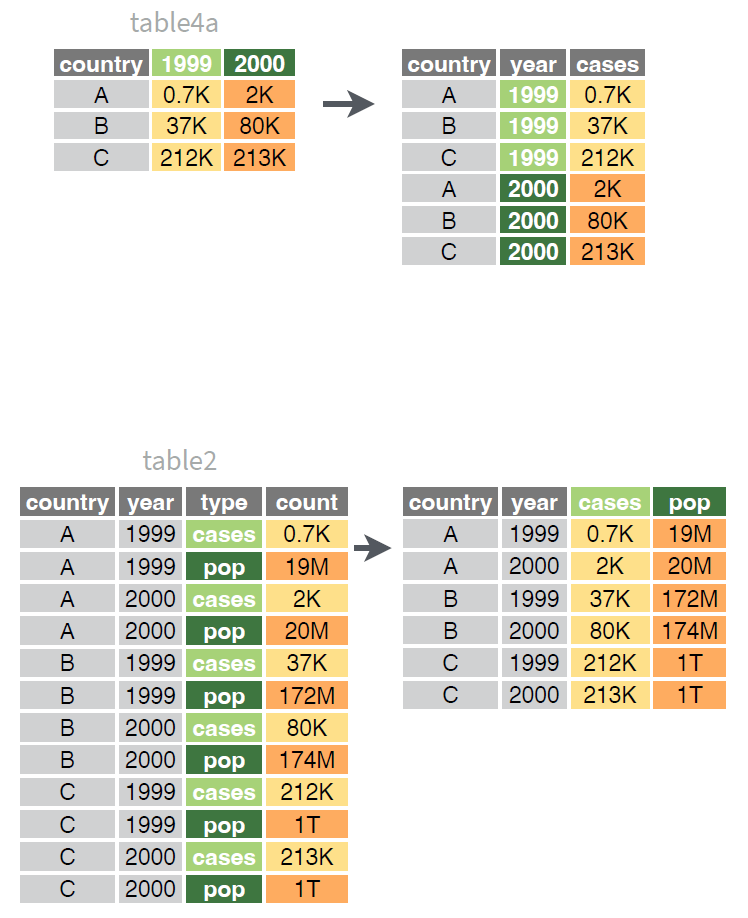
\includegraphics[width=0.7\textwidth,height=\textheight]{./img/posit_pivot_tableonly.png}

}

\caption{Fra bredt til langt og fra langt til bredt --- CC BY SA Posit
Software}

\end{figure}

En pivot: Vi velger de tre årskolonnene og sender \emph{navna} deres til
en ny variabel og \emph{verdiene} deres til en annen. Disse navngir vi
ved en streng. Slik kan det set ut

\begin{Shaded}
\begin{Highlighting}[]
\NormalTok{prognose }\SpecialCharTok{\%\textgreater{}\%} 
  \FunctionTok{pivot\_longer}\NormalTok{(}\AttributeTok{cols =} \FunctionTok{c}\NormalTok{(aar2023, aar2024, aar2025), }
               \AttributeTok{names\_to =} \StringTok{"aar"}\NormalTok{, }
               \AttributeTok{values\_to =} \StringTok{"befolkning"}\NormalTok{)}
\end{Highlighting}
\end{Shaded}

\begin{verbatim}
# A tibble: 24 x 4
   plansone kjonn aar     befolkning
      <int> <chr> <chr>        <dbl>
 1  5001001 M     aar2023        791
 2  5001001 M     aar2024        732
 3  5001001 M     aar2025        673
 4  5001001 K     aar2023        416
 5  5001001 K     aar2024        713
 6  5001001 K     aar2025        750
 7  5001002 M     aar2023        596
 8  5001002 M     aar2024        431
 9  5001002 M     aar2025        503
10  5001002 K     aar2023        442
# ... with 14 more rows
\end{verbatim}

Nå er datasettet \emph{tidy}: hver rad representerer bare én
observasjon. Vi oppnådde dette ved å gå fra vidt til langt format. Når
det er sagt, har vi en del vi kunne ha utsatt på datasettet. Vi kan
bruke det som eksempel på hvordan vi arbeider iterativt, ved å bygge
videre på det vi starter med. Det jeg ikke liker med koden vår over er:

\begin{enumerate}
\def\labelenumi{\arabic{enumi}.}
\tightlist
\item
  Årsvariabelen er en strengvariabel, fordi den fikk med seg bokstavene
  ``aar'' fra kolonnenavnet. Siden år er et tall (strengt tatt dato, men
  det er ikke viktig her), bør den være numerisk. Da kan vi seinere
  summere den opp lettere, samt at vi ikke trenger være redd for at
  sorteringa blir rar.
\item
  Jeg gjentar meg sjøl alt for mye i denne kodeblokken. Legg merke til
  at jeg skriver \texttt{cols\ =\ c(aar2023,\ aar2024,\ aar2025)}. Her
  kunne jeg spart fingra mine en del, siden det er et repetativt
  mønster. Okei, kanskje ikke så mye innsparing her, men hvis vi hadde
  hatt tredve årskolonner ville det begynt å bety noe.
\end{enumerate}

Vi løser nr 1. ved å ta i bruk noen nyttige funksjoner som
\texttt{tidyr}-gjengen har lagt inn i \texttt{pivot()}-funksjonene. Og
nr. 2 ved hjelp av \emph{tidyselect}.

\begin{Shaded}
\begin{Highlighting}[]
\NormalTok{prognose }\OtherTok{\textless{}{-}}\NormalTok{ prognose }\SpecialCharTok{\%\textgreater{}\%} 
  \FunctionTok{pivot\_longer}\NormalTok{(}\AttributeTok{cols =} \FunctionTok{contains}\NormalTok{(}\StringTok{"aar"}\NormalTok{), }
               \AttributeTok{names\_to =} \StringTok{"aar"}\NormalTok{, }
               \AttributeTok{values\_to =} \StringTok{"befolkning"}\NormalTok{, }
               \AttributeTok{names\_prefix =} \StringTok{"aar"}\NormalTok{,}
               \AttributeTok{names\_transform =}\NormalTok{ as.numeric)}

\NormalTok{prognose}
\end{Highlighting}
\end{Shaded}

\begin{verbatim}
# A tibble: 24 x 4
   plansone kjonn   aar befolkning
      <int> <chr> <dbl>      <dbl>
 1  5001001 M      2023        791
 2  5001001 M      2024        732
 3  5001001 M      2025        673
 4  5001001 K      2023        416
 5  5001001 K      2024        713
 6  5001001 K      2025        750
 7  5001002 M      2023        596
 8  5001002 M      2024        431
 9  5001002 M      2025        503
10  5001002 K      2023        442
# ... with 14 more rows
\end{verbatim}

Hva gjorde vi her? Vi brukte \texttt{contains()} i utvelginga av
kolonner for å treffe alle kolonner som inneholdt en viss tekststreng,
her ``aar''. Vi fikk fjerna tekststrengen ``aar'' fra kolonnas
\emph{elementer} ved å si fra til \texttt{pivot\_longer()} at alle
kolonnene vi valgte ut hadde dette prefikset. Til dette brukte vi
\texttt{names\_prefix\ =\ "aar"}. Så gjorde vi om denne kolonna til
numerisk ved å legge på en transformasjon via den enkle
\texttt{as.numeric()}-funksjonen. Dette gjorde vi ved
\texttt{names\_transform\ =\ as.numeric}.

\hypertarget{fra-lang-til-vid}{%
\section{Fra lang til vid}\label{fra-lang-til-vid}}

Sjøl om vi elsker tidy data hender det vi må besudle oss med vide,
rotete data. For eksempel hvis vi har Excel-filer som forventer data på
et visst format. Kanskje de vil ha år bortover. Så det er greit at vi
veit åssen vi går fra lang til vid. Prosessen er stort sett bare det
motsatte av hva vi gjorde med \texttt{pivot\_longer()}, og det minner
meg om dette sitatet fra \emph{Welcome to Nightvale}:

\begin{quote}
And now for a brief public service announcement: Alligators. Can they
kill your children? Yes. Along those lines, to get personal for a
moment, I think the best way to die would be: swallowed by a giant
snake. Going feet first and whole into a slimy maw would give your life
perfect symmetry.
\end{quote}

\begin{Shaded}
\begin{Highlighting}[]
\NormalTok{prognose }\SpecialCharTok{\%\textgreater{}\%} \FunctionTok{pivot\_wider}\NormalTok{(}\AttributeTok{names\_from =}\NormalTok{ aar,}
                         \AttributeTok{names\_prefix =} \StringTok{"aar"}\NormalTok{,}
                         \AttributeTok{values\_from =}\NormalTok{ befolkning)}
\end{Highlighting}
\end{Shaded}

\begin{verbatim}
# A tibble: 8 x 5
  plansone kjonn aar2023 aar2024 aar2025
     <int> <chr>   <dbl>   <dbl>   <dbl>
1  5001001 M         791     732     673
2  5001001 K         416     713     750
3  5001002 M         596     431     503
4  5001002 K         442     486     637
5  5001003 M         538     490     669
6  5001003 K         422     454     475
7  5001004 M         704     646     748
8  5001004 K         493     781     648
\end{verbatim}

\bookmarksetup{startatroot}

\hypertarget{sec-filter}{%
\chapter{Velge rader}\label{sec-filter}}

\begin{Shaded}
\begin{Highlighting}[]
\FunctionTok{library}\NormalTok{(tidyverse)}
\end{Highlighting}
\end{Shaded}

\begin{verbatim}
-- Attaching packages --------------------------------------- tidyverse 1.3.2 --
v ggplot2 3.3.6      v purrr   0.3.5 
v tibble  3.1.8      v dplyr   1.0.10
v tidyr   1.2.1      v stringr 1.4.1 
v readr   2.1.3      v forcats 0.5.2 
-- Conflicts ------------------------------------------ tidyverse_conflicts() --
x dplyr::filter() masks stats::filter()
x dplyr::lag()    masks stats::lag()
\end{verbatim}

Vi skal diskutere utvelgelse av rader, ofte kjent som filtrering.

\hypertarget{filter}{%
\section{Filter}\label{filter}}

Filtre bruker vi svært ofte. De lar oss begrense mengden data vi ser på
og arbeider på. Vi får filtra våre \texttt{dplyr}. Merk at det finnes en
filter-funksjon i \texttt{stats}-pakka som lastes inn når vi starer R,
og dette filteret blir overskrevet av \texttt{dplyr}/\texttt{tidyverse}.
Om du får feilmelding når du bruker filter kan det være at du har glemt
å laste inn \texttt{dplyr}, og at R forsøker å bruke \texttt{stats}'
\texttt{filter()}.

Filtret velger ut \textbf{rader} ved å sjekke ut innholdet i en
\textbf{kolonne}. Vi kan velge ut alle rader som har en viss verdi på en
kolonne. La oss se på at alle menneskene i datasettet \texttt{starwars}.

\begin{Shaded}
\begin{Highlighting}[]
\NormalTok{starwars }\SpecialCharTok{\%\textgreater{}\%} \FunctionTok{filter}\NormalTok{(species }\SpecialCharTok{==} \StringTok{"Human"}\NormalTok{)}
\end{Highlighting}
\end{Shaded}

\begin{verbatim}
# A tibble: 35 x 14
   name        height  mass hair_~1 skin_~2 eye_c~3 birth~4 sex   gender homew~5
   <chr>        <int> <dbl> <chr>   <chr>   <chr>     <dbl> <chr> <chr>  <chr>  
 1 Luke Skywa~    172    77 blond   fair    blue       19   male  mascu~ Tatooi~
 2 Darth Vader    202   136 none    white   yellow     41.9 male  mascu~ Tatooi~
 3 Leia Organa    150    49 brown   light   brown      19   fema~ femin~ Aldera~
 4 Owen Lars      178   120 brown,~ light   blue       52   male  mascu~ Tatooi~
 5 Beru White~    165    75 brown   light   blue       47   fema~ femin~ Tatooi~
 6 Biggs Dark~    183    84 black   light   brown      24   male  mascu~ Tatooi~
 7 Obi-Wan Ke~    182    77 auburn~ fair    blue-g~    57   male  mascu~ Stewjon
 8 Anakin Sky~    188    84 blond   fair    blue       41.9 male  mascu~ Tatooi~
 9 Wilhuff Ta~    180    NA auburn~ fair    blue       64   male  mascu~ Eriadu 
10 Han Solo       180    80 brown   fair    brown      29   male  mascu~ Corell~
# ... with 25 more rows, 4 more variables: species <chr>, films <list>,
#   vehicles <list>, starships <list>, and abbreviated variable names
#   1: hair_color, 2: skin_color, 3: eye_color, 4: birth_year, 5: homeworld
\end{verbatim}

Filteret velger alle radene hvor \textbf{sammenlikninga} vi oppgir er
\texttt{TRUE} (sann). Mer robotisk kan vi si at den i tilfellet over
velger rader hvor cella under kolonna \emph{species} tilfredsstiller
betingelsen ``innholdet i cella er lik \emph{Human}''. Dermed kan vi
oppgi andre uttrykk som evalueres til enten \texttt{TRUE} eller
\texttt{FALSE}. Hva med å hente ut alle som er høyere enn 170 cm?

\begin{Shaded}
\begin{Highlighting}[]
\NormalTok{starwars }\SpecialCharTok{\%\textgreater{}\%} \FunctionTok{filter}\NormalTok{(height }\SpecialCharTok{\textgreater{}} \DecValTok{170}\NormalTok{)}
\end{Highlighting}
\end{Shaded}

\begin{verbatim}
# A tibble: 54 x 14
   name        height  mass hair_~1 skin_~2 eye_c~3 birth~4 sex   gender homew~5
   <chr>        <int> <dbl> <chr>   <chr>   <chr>     <dbl> <chr> <chr>  <chr>  
 1 Luke Skywa~    172    77 blond   fair    blue       19   male  mascu~ Tatooi~
 2 Darth Vader    202   136 none    white   yellow     41.9 male  mascu~ Tatooi~
 3 Owen Lars      178   120 brown,~ light   blue       52   male  mascu~ Tatooi~
 4 Biggs Dark~    183    84 black   light   brown      24   male  mascu~ Tatooi~
 5 Obi-Wan Ke~    182    77 auburn~ fair    blue-g~    57   male  mascu~ Stewjon
 6 Anakin Sky~    188    84 blond   fair    blue       41.9 male  mascu~ Tatooi~
 7 Wilhuff Ta~    180    NA auburn~ fair    blue       64   male  mascu~ Eriadu 
 8 Chewbacca      228   112 brown   unknown blue      200   male  mascu~ Kashyy~
 9 Han Solo       180    80 brown   fair    brown      29   male  mascu~ Corell~
10 Greedo         173    74 <NA>    green   black      44   male  mascu~ Rodia  
# ... with 44 more rows, 4 more variables: species <chr>, films <list>,
#   vehicles <list>, starships <list>, and abbreviated variable names
#   1: hair_color, 2: skin_color, 3: eye_color, 4: birth_year, 5: homeworld
\end{verbatim}

Vi kan oppgi flere betingelser. Hva med alle kvinnelige mennesker?

\begin{Shaded}
\begin{Highlighting}[]
\NormalTok{starwars }\SpecialCharTok{\%\textgreater{}\%} \FunctionTok{filter}\NormalTok{(species }\SpecialCharTok{==} \StringTok{"Human"} \SpecialCharTok{\&}\NormalTok{ sex }\SpecialCharTok{==} \StringTok{"female"}\NormalTok{)}
\end{Highlighting}
\end{Shaded}

\begin{verbatim}
# A tibble: 9 x 14
  name         height  mass hair_~1 skin_~2 eye_c~3 birth~4 sex   gender homew~5
  <chr>         <int> <dbl> <chr>   <chr>   <chr>     <dbl> <chr> <chr>  <chr>  
1 Leia Organa     150    49 brown   light   brown        19 fema~ femin~ Aldera~
2 Beru Whites~    165    75 brown   light   blue         47 fema~ femin~ Tatooi~
3 Mon Mothma      150    NA auburn  fair    blue         48 fema~ femin~ Chandr~
4 Shmi Skywal~    163    NA black   fair    brown        72 fema~ femin~ Tatooi~
5 Cordé           157    NA brown   light   brown        NA fema~ femin~ Naboo  
6 Dormé           165    NA brown   light   brown        NA fema~ femin~ Naboo  
7 Jocasta Nu      167    NA white   fair    blue         NA fema~ femin~ Corusc~
8 Rey              NA    NA brown   light   hazel        NA fema~ femin~ <NA>   
9 Padmé Amida~    165    45 brown   light   brown        46 fema~ femin~ Naboo  
# ... with 4 more variables: species <chr>, films <list>, vehicles <list>,
#   starships <list>, and abbreviated variable names 1: hair_color,
#   2: skin_color, 3: eye_color, 4: birth_year, 5: homeworld
\end{verbatim}

Ikke så veldig mange. Ikke rart Star Wars filer Bechdel-testen. Får vi
med flere hvis vi ikke skiller mellom sex og gender? Altså at vi tar med
dem er \emph{enten} female \emph{eller} feminine?

\begin{Shaded}
\begin{Highlighting}[]
\NormalTok{starwars }\SpecialCharTok{\%\textgreater{}\%} \FunctionTok{filter}\NormalTok{(species }\SpecialCharTok{==} \StringTok{"Human"} \SpecialCharTok{\&}\NormalTok{ (sex }\SpecialCharTok{==} \StringTok{"female"} \SpecialCharTok{|}\NormalTok{ gender }\SpecialCharTok{==} \StringTok{"feminine"}\NormalTok{))}
\end{Highlighting}
\end{Shaded}

\begin{verbatim}
# A tibble: 9 x 14
  name         height  mass hair_~1 skin_~2 eye_c~3 birth~4 sex   gender homew~5
  <chr>         <int> <dbl> <chr>   <chr>   <chr>     <dbl> <chr> <chr>  <chr>  
1 Leia Organa     150    49 brown   light   brown        19 fema~ femin~ Aldera~
2 Beru Whites~    165    75 brown   light   blue         47 fema~ femin~ Tatooi~
3 Mon Mothma      150    NA auburn  fair    blue         48 fema~ femin~ Chandr~
4 Shmi Skywal~    163    NA black   fair    brown        72 fema~ femin~ Tatooi~
5 Cordé           157    NA brown   light   brown        NA fema~ femin~ Naboo  
6 Dormé           165    NA brown   light   brown        NA fema~ femin~ Naboo  
7 Jocasta Nu      167    NA white   fair    blue         NA fema~ femin~ Corusc~
8 Rey              NA    NA brown   light   hazel        NA fema~ femin~ <NA>   
9 Padmé Amida~    165    45 brown   light   brown        46 fema~ femin~ Naboo  
# ... with 4 more variables: species <chr>, films <list>, vehicles <list>,
#   starships <list>, and abbreviated variable names 1: hair_color,
#   2: skin_color, 3: eye_color, 4: birth_year, 5: homeworld
\end{verbatim}

Nei.

Men vi fikk illustrert filteret. Vi bruker noen logiske operatorer for å
kombinere ulike ledd i betingelsene våre.

\begin{itemize}
\tightlist
\item
  \texttt{\&}: \textbf{og}. Både x og y må være tilfredsstilt.
\item
  \texttt{\textbar{}}: \textbf{eller}. Enten x eller y må være
  tilfredsstilt.
\item
  \texttt{==}: \textbf{er lik}. x må være lik y.
\item
  \texttt{!=}: \textbf{er ikke lik}. x må være ulik y.
\item
  \texttt{\textless{}} og \texttt{\textgreater{}}: \textbf{mindre enn}
  og \textbf{større enn}
\item
  \texttt{\textless{}=} og \texttt{\textgreater{}=}: \textbf{mindre enn
  eller lik} og \textbf{større enn eller lik}.
\end{itemize}

Og vi bruker \texttt{()} for å gruppere betingelser sammen. La oss se på
hva som skjer med antall rader som blir tatt med når vi fjerner
\texttt{()}.

\begin{Shaded}
\begin{Highlighting}[]
\CommentTok{\# Med () rundt female og feminine}
\NormalTok{starwars }\SpecialCharTok{\%\textgreater{}\%} 
  \FunctionTok{filter}\NormalTok{(species }\SpecialCharTok{==} \StringTok{"Human"} \SpecialCharTok{\&}\NormalTok{ (sex }\SpecialCharTok{==} \StringTok{"female"} \SpecialCharTok{|}\NormalTok{ gender }\SpecialCharTok{==} \StringTok{"feminine"}\NormalTok{)) }\SpecialCharTok{\%\textgreater{}\%} 
  \FunctionTok{nrow}\NormalTok{()}
\end{Highlighting}
\end{Shaded}

\begin{verbatim}
[1] 9
\end{verbatim}

\begin{Shaded}
\begin{Highlighting}[]
\CommentTok{\# Uten ()}
\NormalTok{starwars }\SpecialCharTok{\%\textgreater{}\%} 
  \FunctionTok{filter}\NormalTok{(species }\SpecialCharTok{==} \StringTok{"Human"} \SpecialCharTok{\&}\NormalTok{ sex }\SpecialCharTok{==} \StringTok{"female"} \SpecialCharTok{|}\NormalTok{ gender }\SpecialCharTok{==} \StringTok{"feminine"}\NormalTok{) }\SpecialCharTok{\%\textgreater{}\%} 
  \FunctionTok{nrow}\NormalTok{()}
\end{Highlighting}
\end{Shaded}

\begin{verbatim}
[1] 17
\end{verbatim}

I det første eksemplet må du være 1) menneske \emph{og} 2)
\textbf{enten} female \emph{eller} feminine. I det andre eksemplet må du
være 1) menneske \textbf{og} female \textbf{eller} 2) feminine. Dermed
får vi med oss en del roboter og romvesener som er feminine i det andre
eksemplet.

Vi bruker ofte filtre for å fjerne deler av et datasett, for eksempel
dersom vi bare vil se på Trondheim. Da filtrer vi kanskje med ei kolonne
som inneholder

\begin{itemize}
\tightlist
\item
  kommunnummeret til Trondheim (5001),
\item
  det gamle kommunenummeret til Trondheim (1601),
\item
  en tekststreng med navet til byen (``Trondheim''),
\item
  en tekststreng med det gamle navnet på byen (``Trondhjem''),
\item
  en tekststreng med navnet på byen uten stor forbokstav
  (``Trondheim''), eller
\item
  en tekststreng med navnet på byen feilstava (``Trodnheim'').
\item
  en tekststreng med navnet på byen og noe tilleggstekst som vi ikke
  trenger (``Trondheim by'')
\end{itemize}

Antakelig ikke alle på en gang, men det er greit å vite hvordan man gjør
en \textbf{delvis match}. Spesielt når vi får en liste med navn på ting
som må matches med våre egne data er det typisk at de skriver navna noe
annerledes enn oss. Dette er gjerne fordi det ikke egentlig er noen
standard måte å skrive navna på, eller fordi navna endres.
Barnehagedatasett er et typisk eksempel her.

Å matche på ulike numre handler vanligvis om å sette sammen en serie med
\emph{eller} betingelser via \texttt{\textbar{}}. Vi fokuserer derfor på
tekststrenger. Til dette finner vi en svært nyttig pakke som heter
\texttt{stringr}.

\begin{figure}

{\centering 
\includegraphics[width=0.4\textwidth,height=\textheight]{./img/Stringer_Bell.jpg}

}

\caption{Pakka handler ikke om å selge dop i Baltimore, men om å
håndtere tekststrenger.}

\end{figure}

\hypertarget{stringr}{%
\section{Stringr}\label{stringr}}

\texttt{stringr} har drøssevis av nyttige funksjoner for oss, og vi har
så klart ikke tid å gå innom alt. En del av funksjonene baserer seg på
noe som kalles regulære uttrykk (\emph{regular expressions}), ofte
henvist til som \textbf{regex}. Regex er serier med tegn som
spesifiserer et spesifikt mønster. Det brukes når vi vil ha treff på
flere varianter.

Under bruker jeg regex for å treffe på to skrivemåter av Trondheim. Vi
bruker \texttt{str\_detect()} for å detektere strenger i en kolonne som
matcher et mønster. Mønsteret er altså Trondheim eller Trondhjem. Siden
den eneste forskjellen på disse to er om vi bruker \emph{ei} eller
\emph{je} i slutten, kan vi skrive dette som
\texttt{"Trondh(ei\textbar{}je)m"}.

\begin{Shaded}
\begin{Highlighting}[]
\CommentTok{\# Lager et fiktivt lite datasett}
\NormalTok{byer }\OtherTok{\textless{}{-}} \FunctionTok{tibble}\NormalTok{(}
  \AttributeTok{by =} \FunctionTok{c}\NormalTok{(}\StringTok{"Trondheim"}\NormalTok{, }\StringTok{"Trondhjem"}\NormalTok{, }\StringTok{"Drammen"}\NormalTok{),}
  \AttributeTok{valuta =} \FunctionTok{c}\NormalTok{(}\StringTok{"NOK"}\NormalTok{, }\StringTok{"riksdaler"}\NormalTok{, }\StringTok{"NOK"}\NormalTok{)}
\NormalTok{)}

\CommentTok{\# Filter ved hjelp av regex}
\NormalTok{byer }\SpecialCharTok{\%\textgreater{}\%} 
  \FunctionTok{filter}\NormalTok{(}\FunctionTok{str\_detect}\NormalTok{(by, }\StringTok{"Trondh(ei|je)m"}\NormalTok{))}
\end{Highlighting}
\end{Shaded}

\begin{verbatim}
# A tibble: 2 x 2
  by        valuta   
  <chr>     <chr>    
1 Trondheim NOK      
2 Trondhjem riksdaler
\end{verbatim}

\begin{Shaded}
\begin{Highlighting}[]
\CommentTok{\# En mindre effektiv måte å gjøre dette på ville vært}
\NormalTok{byer }\SpecialCharTok{\%\textgreater{}\%} 
  \FunctionTok{filter}\NormalTok{(by }\SpecialCharTok{==} \StringTok{"Trondheim"} \SpecialCharTok{|}\NormalTok{ by }\SpecialCharTok{==} \StringTok{"Trondhjem"}\NormalTok{)}
\end{Highlighting}
\end{Shaded}

\begin{verbatim}
# A tibble: 2 x 2
  by        valuta   
  <chr>     <chr>    
1 Trondheim NOK      
2 Trondhjem riksdaler
\end{verbatim}

Du kan spørre deg hvorfor det andre eksemplet er mindre effektivt når
det bare koster oss noen få ekstra tegn. Fordi jeg må gjenta meg sjøl
når jeg skriver \texttt{by\ ==} og \texttt{Trondh}. Akkurat i dette
tilfellet er det ikke særlig alvorlig. Men når vi utvider og får større
datasett og mer avanserte søkemønstre vil det begynne å gjøre seg
gjeldende. En ting er at vi sparer tid på skrive mindre. En annen ting
er at det blir lettere å gjøre endringer seinere. Fordi vi ikke må endre
en serie med \emph{eller}-betingelser, men kun den ene regex-en.

Alle funksjonene i \texttt{stringr} starter med \texttt{str\_}, som gjør
dem lett å søke opp. Nyttig, for det er mange av dem! De jeg bruker
oftest er

\begin{itemize}
\tightlist
\item
  \texttt{str\_sub()} for å hente ut en del av en streng
\item
  \texttt{str\_detect()} i kombinasjon med \texttt{filter()} for å finne
  en delvis match i en kolonne
\item
  \texttt{str\_replace()} for å erstatte del av en streng med noe annet
\item
  \texttt{str\_to\_lower()} og \texttt{str\_to\_upper()} for å fjerne
  feilkilder når jeg søker. Spesielt den første er nyttig. Hvis jeg skal
  matche på navn vil jeg unngå at jeg får ikke-match bare fordi noen
  navn har store bokstaver enkelte steder mens andre ikke. Jeg vil at
  ``Byåsen barnehage'' skal matche med \texttt{Byåsen\ Barnehage}. Merk
  at det finnes varianter av disse i \texttt{base\ R} også.
\end{itemize}

La oss se noen eksempler på bruk av disse

\begin{Shaded}
\begin{Highlighting}[]
\CommentTok{\# Hent ut de fire første bokstavene av en kolonne}
\NormalTok{byer }\SpecialCharTok{\%\textgreater{}\%} 
  \FunctionTok{mutate}\NormalTok{(}\AttributeTok{by4 =} \FunctionTok{str\_sub}\NormalTok{(by, }\DecValTok{1}\NormalTok{, }\DecValTok{4}\NormalTok{))}
\end{Highlighting}
\end{Shaded}

\begin{verbatim}
# A tibble: 3 x 3
  by        valuta    by4  
  <chr>     <chr>     <chr>
1 Trondheim NOK       Tron 
2 Trondhjem riksdaler Tron 
3 Drammen   NOK       Dram 
\end{verbatim}

\begin{Shaded}
\begin{Highlighting}[]
\CommentTok{\# Bytt ut deler av en streng}
\NormalTok{byer }\SpecialCharTok{\%\textgreater{}\%} 
  \FunctionTok{mutate}\NormalTok{(}\AttributeTok{nytt\_bynavn =} \FunctionTok{str\_replace}\NormalTok{(by, }\StringTok{"Trond"}\NormalTok{, }\StringTok{"Trønder"}\NormalTok{))}
\end{Highlighting}
\end{Shaded}

\begin{verbatim}
# A tibble: 3 x 3
  by        valuta    nytt_bynavn
  <chr>     <chr>     <chr>      
1 Trondheim NOK       Trønderheim
2 Trondhjem riksdaler Trønderhjem
3 Drammen   NOK       Drammen    
\end{verbatim}

\begin{Shaded}
\begin{Highlighting}[]
\CommentTok{\# Gjøre om en kolonne til små bokstaver. }
\NormalTok{byer }\SpecialCharTok{\%\textgreater{}\%} 
  \FunctionTok{mutate}\NormalTok{(}\AttributeTok{valuta\_lower =} \FunctionTok{str\_to\_lower}\NormalTok{(valuta))}
\end{Highlighting}
\end{Shaded}

\begin{verbatim}
# A tibble: 3 x 3
  by        valuta    valuta_lower
  <chr>     <chr>     <chr>       
1 Trondheim NOK       nok         
2 Trondhjem riksdaler riksdaler   
3 Drammen   NOK       nok         
\end{verbatim}

\texttt{stringr} har mange muligheter i seg. Spesielt bruken av regex er
svært nyttig, som nevnt over. Men læringskurva er bratt. Og særlig det å
søke etter tall i en tekststreng. Noen nyttige funksjoner her er å
kombinere tegntype og kvantitet. Sjekk ut side to av
\texttt{stringr}-\href{https://posit.co/resources/cheatsheets/}{jukselappen
til Posit}.

Her lager jeg et rart datasett for å vise hvordan vi kan bruke disse
regex-kommandoene. Datasettet blir laga ved å sette sammen tilfeldige
serier med tall og bokstaver som vi seinere kan søke på. Her bruker jeg
\texttt{set.seed()} for å sørge for at de påfølgende randomiserte
prosessene blir like hver gang de kjøres. Slik at du og jeg ser de samme
talla hver gang.

\begin{Shaded}
\begin{Highlighting}[]
\FunctionTok{set.seed}\NormalTok{(}\DecValTok{123}\NormalTok{)}

\CommentTok{\# En funksjon som lager en serie av siffer og bokstaver av ulik lengde.}
\NormalTok{lag\_streng }\OtherTok{\textless{}{-}} \ControlFlowTok{function}\NormalTok{() \{}
\NormalTok{  tall }\OtherTok{\textless{}{-}} \FunctionTok{seq}\NormalTok{(}\DecValTok{1}\SpecialCharTok{:}\DecValTok{10}\NormalTok{) }\SpecialCharTok{\%\textgreater{}\%} \FunctionTok{as.character}\NormalTok{()}
\NormalTok{  bokstaver }\OtherTok{\textless{}{-}}\NormalTok{ letters[}\DecValTok{1}\SpecialCharTok{:}\DecValTok{10}\NormalTok{]}
\NormalTok{  tall\_bokstaver }\OtherTok{\textless{}{-}} \FunctionTok{c}\NormalTok{(tall, bokstaver)}
  
  \FunctionTok{paste0}\NormalTok{(}\FunctionTok{sample}\NormalTok{(tall\_bokstaver, }\AttributeTok{size =} \FunctionTok{runif}\NormalTok{(}\DecValTok{1}\NormalTok{, }\DecValTok{3}\NormalTok{, }\DecValTok{5}\NormalTok{), }\AttributeTok{replace =} \ConstantTok{TRUE}\NormalTok{), }\AttributeTok{collapse =} \StringTok{""}\NormalTok{)}
\NormalTok{\}}

\FunctionTok{set.seed}\NormalTok{(}\DecValTok{123}\NormalTok{)}

\CommentTok{\# Setter det sammen i et datasett.  }
\NormalTok{utvalg }\OtherTok{\textless{}{-}} \FunctionTok{tibble}\NormalTok{(}
  \AttributeTok{id =} \FunctionTok{seq}\NormalTok{(}\DecValTok{1}\SpecialCharTok{:}\DecValTok{200}\NormalTok{), }
  \AttributeTok{name =} \FunctionTok{replicate}\NormalTok{(}\DecValTok{200}\NormalTok{, }\FunctionTok{lag\_streng}\NormalTok{())}
\NormalTok{)}

\CommentTok{\# Slik ser det ut. }
\NormalTok{utvalg}
\end{Highlighting}
\end{Shaded}

\begin{verbatim}
# A tibble: 200 x 2
      id name 
   <int> <chr>
 1     1 eid  
 2     2 10ha5
 3     3 d5i9 
 4     4 38710
 5     5 i4dg 
 6     6 7be10
 7     7 799  
 8     8 762  
 9     9 58b  
10    10 ch1  
# ... with 190 more rows
\end{verbatim}

\begin{Shaded}
\begin{Highlighting}[]
\CommentTok{\# La oss finne de navna hvor det er to bokstaver etterfulgt av to nummer}
\NormalTok{utvalg }\SpecialCharTok{\%\textgreater{}\%} 
  \FunctionTok{filter}\NormalTok{(}\FunctionTok{str\_detect}\NormalTok{(name, }\StringTok{"[[:alpha:]]\{2\}[[:digit:]]\{2\}"}\NormalTok{))}
\end{Highlighting}
\end{Shaded}

\begin{verbatim}
# A tibble: 12 x 2
      id name  
   <int> <chr> 
 1     6 7be10 
 2    16 jd38  
 3    32 bg10  
 4    43 dd61  
 5    49 ch106 
 6    52 hg12  
 7    56 ff34  
 8    77 bc1010
 9    97 2fi10 
10   155 hhj10 
11   162 af54  
12   189 cd29  
\end{verbatim}

Dette mønstret ser overveldende ut, så la oss pakke det ut:
\texttt{"{[}{[}:alpha:{]}{]}\{2\}{[}{[}:digit:{]}{]}\{2\}"}

\begin{itemize}
\tightlist
\item
  \texttt{{[}{[}:alpha:{]}{]}} treffer alle bokstaver.
\item
  \texttt{{[}{[}:digit:{]}{]}} treffer alle tall.
\item
  \texttt{\{2\}} betyr nøyaktig to forekomster av det som kom før meg.
  Vi bruker den både for bokstaver og tall. Alternativet ville vært å
  skrevet f.eks. \texttt{{[}{[}:alpha:{]}{]}{[}{[}:alpha:{]}{]}}
\end{itemize}

Det er verdt å tenke litt på tegnkoding igjen. Hvordan lagres
informasjon om tall og bokstaver på pc-en? Hvordan behandles tall og
bokstaver (og symboler) annerledes av programmeringsspråk som R? En
tallserie vil f.eks. sorteres annerledes avhengig av om den er koda som
numerisk eller streng.

\begin{Shaded}
\begin{Highlighting}[]
\CommentTok{\# En vektor som inneholder en serie fra 1 til 24 i tilfeldig rekkefølge}
\NormalTok{tall }\OtherTok{\textless{}{-}} \FunctionTok{sample}\NormalTok{(}\FunctionTok{c}\NormalTok{(}\DecValTok{1}\SpecialCharTok{:}\DecValTok{24}\NormalTok{), }\DecValTok{24}\NormalTok{)}

\CommentTok{\# Vi sortere den først når den er numerisk og deretter når den er en streng.}
\NormalTok{tall }\SpecialCharTok{\%\textgreater{}\%} \FunctionTok{sort}\NormalTok{()}
\end{Highlighting}
\end{Shaded}

\begin{verbatim}
 [1]  1  2  3  4  5  6  7  8  9 10 11 12 13 14 15 16 17 18 19 20 21 22 23 24
\end{verbatim}

\begin{Shaded}
\begin{Highlighting}[]
\NormalTok{tall }\SpecialCharTok{\%\textgreater{}\%} \FunctionTok{as.character}\NormalTok{() }\SpecialCharTok{\%\textgreater{}\%} \FunctionTok{sort}\NormalTok{()}
\end{Highlighting}
\end{Shaded}

\begin{verbatim}
 [1] "1"  "10" "11" "12" "13" "14" "15" "16" "17" "18" "19" "2"  "20" "21" "22"
[16] "23" "24" "3"  "4"  "5"  "6"  "7"  "8"  "9" 
\end{verbatim}

I neste kodeblokk lager jeg to datasett. Det første er likt det vi hadde
i sted, foruten at jeg kun henter ut de første ti radene. Det andre
datasettet er likt dette, foruten at jeg har bedt om \emph{kun ett
siffer (digit)} på slutten. For å vise tydeligere hva som skjer binder
jeg de to radene sammen.

\begin{Shaded}
\begin{Highlighting}[]
\NormalTok{foo }\OtherTok{\textless{}{-}}\NormalTok{ utvalg }\SpecialCharTok{\%\textgreater{}\%} 
  \FunctionTok{filter}\NormalTok{(}\FunctionTok{str\_detect}\NormalTok{(name, }\StringTok{"[[:alpha:]]\{2\}[[:digit:]]\{2\}"}\NormalTok{)) }\SpecialCharTok{\%\textgreater{}\%} 
  \FunctionTok{slice}\NormalTok{(}\DecValTok{1}\SpecialCharTok{:}\DecValTok{10}\NormalTok{)}

\NormalTok{bar }\OtherTok{\textless{}{-}}\NormalTok{ utvalg }\SpecialCharTok{\%\textgreater{}\%} 
  \FunctionTok{filter}\NormalTok{(}\FunctionTok{str\_detect}\NormalTok{(name, }\StringTok{"[[:alpha:]]\{2\}[[:digit:]]\{1\}"}\NormalTok{)) }\SpecialCharTok{\%\textgreater{}\%} 
  \FunctionTok{slice}\NormalTok{(}\DecValTok{1}\SpecialCharTok{:}\DecValTok{10}\NormalTok{)}

\FunctionTok{bind\_cols}\NormalTok{(foo, bar)}
\end{Highlighting}
\end{Shaded}

\begin{verbatim}
New names:
* `id` -> `id...1`
* `name` -> `name...2`
* `id` -> `id...3`
* `name` -> `name...4`
\end{verbatim}

\begin{verbatim}
# A tibble: 10 x 4
   id...1 name...2 id...3 name...4
    <int> <chr>     <int> <chr>   
 1      6 7be10         2 10ha5   
 2     16 jd38          6 7be10   
 3     32 bg10         10 ch1     
 4     43 dd61         12 fj6     
 5     49 ch106        14 hg2     
 6     52 hg12         16 jd38    
 7     56 ff34         17 bd3d    
 8     77 bc1010       21 gd3     
 9     97 2fi10        23 ga7     
10    155 hhj10        26 fa4b    
\end{verbatim}

Legg merke til kolonna helt til høyre. Vi ba om kun ett siffer, likevel
får vi ``7be10'' og ``jd38''. Hvorfor? Fordi de inneholder, nettopp
``ett siffer''. Dette sifferet er tilfeldigvis etterfulgt av et annet
siffer, men det sa vi ikke spesifikt at vi skulle unngå. Her gjorde jeg
en antakelse som viste seg å ikke stemme. Det var en antakelse jeg ikke
var helt bevisst at jeg gjorde, og det var at koden min skulle vise meg
rader som inneholder to bokstaver og ett, og kun ett, ikke to eller
flere, siffer.

Vi ser det samme skjer med den første kolonna også: her får vi treff på
to bokstaver etterfulgt av tre og fire siffer. Hvis vi skulle fiksa
koden til å treffe på ``to bokstaver etterfulgt av kun to og ikke flere
siffer'' kunne vi endra det slik:

\begin{Shaded}
\begin{Highlighting}[]
\NormalTok{utvalg }\SpecialCharTok{\%\textgreater{}\%} 
  \FunctionTok{filter}\NormalTok{(}\FunctionTok{str\_detect}\NormalTok{(name, }\StringTok{"[[:alpha:]]\{2\}[[:digit:]]\{2\}(?![[:digit:]])"}\NormalTok{))}
\end{Highlighting}
\end{Shaded}

\begin{verbatim}
# A tibble: 10 x 2
      id name 
   <int> <chr>
 1     6 7be10
 2    16 jd38 
 3    32 bg10 
 4    43 dd61 
 5    52 hg12 
 6    56 ff34 
 7    97 2fi10
 8   155 hhj10
 9   162 af54 
10   189 cd29 
\end{verbatim}

Det jeg håper på å få fram her er at vi må stoppe opp innimellom og
teste våre egne antakelser og arbeid.

\hypertarget{select}{%
\section{Select}\label{select}}

Vi har brukt \texttt{select()} før, se Kapittel~\ref{sec-select}. Den er
nyttig å ta opp igjen her. Med \texttt{select()} kan vi velge ut
kolonner og med \texttt{filter()} kan vi velge ut rader. Dermed er det
ofte nyttig å bruke begge sammen. Jeg bruker dem spesielt mye når jeg
gjør en første gjennomgang av et skript. Da velger jeg ut kun de radene
og kolonnene som jeg er interessert i og arbeider på dem. Dette gjør det
lettere å se om koden min funker, uten å måtte se for mye urelevant. Når
jeg veit at skriptet funker, kan jeg gå tilbake og fjerne
\texttt{select()} og \texttt{filter()} slik at hele datasettet kjøres
gjennom skriptet.

Det er nyttig å vite at vi kan bruke noen liknende streng-teknikker på
\texttt{select()} som vi brukte på \texttt{filter()}. Vi henter inn et
nytt, simulert datasett hvor den del av kolonnene våre har navn på samme
form.

\begin{Shaded}
\begin{Highlighting}[]
\NormalTok{prognose }\OtherTok{\textless{}{-}} \FunctionTok{tibble}\NormalTok{(}
  \AttributeTok{plansone =} \FunctionTok{rep}\NormalTok{(}\FunctionTok{seq}\NormalTok{(}\DecValTok{5001001}\NormalTok{, }\DecValTok{5001004}\NormalTok{), }\AttributeTok{each =} \DecValTok{2}\NormalTok{),}
  \AttributeTok{kjonn =} \FunctionTok{rep}\NormalTok{(}\FunctionTok{c}\NormalTok{(}\StringTok{"M"}\NormalTok{, }\StringTok{"K"}\NormalTok{), }\DecValTok{4}\NormalTok{),}
  \AttributeTok{aar2023 =} \FunctionTok{round}\NormalTok{(}\FunctionTok{runif}\NormalTok{(}\DecValTok{8}\NormalTok{, }\DecValTok{400}\NormalTok{, }\DecValTok{800}\NormalTok{)),}
  \AttributeTok{aar2024 =} \FunctionTok{round}\NormalTok{(}\FunctionTok{runif}\NormalTok{(}\DecValTok{8}\NormalTok{, }\DecValTok{400}\NormalTok{, }\DecValTok{800}\NormalTok{)),}
  \AttributeTok{aar2025 =} \FunctionTok{round}\NormalTok{(}\FunctionTok{runif}\NormalTok{(}\DecValTok{8}\NormalTok{, }\DecValTok{400}\NormalTok{, }\DecValTok{800}\NormalTok{))}
\NormalTok{) }\SpecialCharTok{\%\textgreater{}\%} 
  \FunctionTok{tibble}\NormalTok{(}
    \AttributeTok{faktisk2023 =} \FunctionTok{round}\NormalTok{(aar2023 }\SpecialCharTok{+}\NormalTok{ aar2023 }\SpecialCharTok{*}\NormalTok{ (}\FunctionTok{rnorm}\NormalTok{(}\DecValTok{1}\NormalTok{, }\DecValTok{0}\NormalTok{, }\DecValTok{10}\NormalTok{)}\SpecialCharTok{/}\DecValTok{100}\NormalTok{)),}
    \AttributeTok{faktisk2024 =} \FunctionTok{round}\NormalTok{(aar2024 }\SpecialCharTok{+}\NormalTok{ aar2024 }\SpecialCharTok{*}\NormalTok{ (}\FunctionTok{rnorm}\NormalTok{(}\DecValTok{1}\NormalTok{, }\DecValTok{0}\NormalTok{, }\DecValTok{10}\NormalTok{)}\SpecialCharTok{/}\DecValTok{100}\NormalTok{)),}
    \AttributeTok{faktisk2025 =} \FunctionTok{round}\NormalTok{(aar2025 }\SpecialCharTok{+}\NormalTok{ aar2025 }\SpecialCharTok{*}\NormalTok{ (}\FunctionTok{rnorm}\NormalTok{(}\DecValTok{1}\NormalTok{, }\DecValTok{0}\NormalTok{, }\DecValTok{10}\NormalTok{)}\SpecialCharTok{/}\DecValTok{100}\NormalTok{))}
\NormalTok{  )}
\NormalTok{prognose}
\end{Highlighting}
\end{Shaded}

\begin{verbatim}
# A tibble: 8 x 8
  plansone kjonn aar2023 aar2024 aar2025 faktisk2023 faktisk2024 faktisk2025
     <int> <chr>   <dbl>   <dbl>   <dbl>       <dbl>       <dbl>       <dbl>
1  5001001 M         460     550     753         453         545         785
2  5001001 K         472     781     475         464         773         495
3  5001002 M         536     408     486         527         404         506
4  5001002 K         474     645     748         466         639         779
5  5001003 M         562     585     424         553         579         442
6  5001003 K         645     542     494         635         537         515
7  5001004 M         674     753     797         663         746         831
8  5001004 K         729     430     671         717         426         699
\end{verbatim}

Her har vi kun tre av hver kolonne, men se for dere at vi hadde hatt
tredve. Da ville det vært nyttig å slippe å skrive inn navnet på hver
enkelt.

La oss si at vi vil ha tak i kun de faktiske befolkningstalla, altså de
kolonnene som har ``faktisk'' i navnet. Vi kan bruke \texttt{contains()}
eller \texttt{matches()} inni \texttt{select()}.

\begin{Shaded}
\begin{Highlighting}[]
\NormalTok{prognose }\SpecialCharTok{\%\textgreater{}\%} 
  \FunctionTok{select}\NormalTok{(}\FunctionTok{contains}\NormalTok{(}\StringTok{"faktisk"}\NormalTok{))}
\end{Highlighting}
\end{Shaded}

\begin{verbatim}
# A tibble: 8 x 3
  faktisk2023 faktisk2024 faktisk2025
        <dbl>       <dbl>       <dbl>
1         453         545         785
2         464         773         495
3         527         404         506
4         466         639         779
5         553         579         442
6         635         537         515
7         663         746         831
8         717         426         699
\end{verbatim}

Hva er forskjellen på dem? \texttt{matches()} lar oss bruke en regex. Si
at vi vil ha kolonner med ``faktisk'' i navnet, etterfulgt av en eller
flere siffer, og som slutter på 5.

\begin{Shaded}
\begin{Highlighting}[]
\NormalTok{prognose }\SpecialCharTok{\%\textgreater{}\%} 
  \FunctionTok{select}\NormalTok{(}\FunctionTok{matches}\NormalTok{(}\StringTok{"faktisk[[:digit:]]+5$"}\NormalTok{))}
\end{Highlighting}
\end{Shaded}

\begin{verbatim}
# A tibble: 8 x 1
  faktisk2025
        <dbl>
1         785
2         495
3         506
4         779
5         442
6         515
7         831
8         699
\end{verbatim}

Jeg bruker ofte \texttt{select()} til å endre rekkefølgen på kolonner.
Ofte vil jeg ha den kolonna jeg nettopp lagde fremst. Da er det nyttig å
huske på noen av triksa fra \emph{tidy evaluation}:
\texttt{everything()}. Den lar meg slippe å skrive opp alle kolonnene i
datasettet:

\begin{Shaded}
\begin{Highlighting}[]
\NormalTok{prognose }\SpecialCharTok{\%\textgreater{}\%} 
  \FunctionTok{select}\NormalTok{(plansone, faktisk2025, }\FunctionTok{everything}\NormalTok{())}
\end{Highlighting}
\end{Shaded}

\begin{verbatim}
# A tibble: 8 x 8
  plansone faktisk2025 kjonn aar2023 aar2024 aar2025 faktisk2023 faktisk2024
     <int>       <dbl> <chr>   <dbl>   <dbl>   <dbl>       <dbl>       <dbl>
1  5001001         785 M         460     550     753         453         545
2  5001001         495 K         472     781     475         464         773
3  5001002         506 M         536     408     486         527         404
4  5001002         779 K         474     645     748         466         639
5  5001003         442 M         562     585     424         553         579
6  5001003         515 K         645     542     494         635         537
7  5001004         831 M         674     753     797         663         746
8  5001004         699 K         729     430     671         717         426
\end{verbatim}

\bookmarksetup{startatroot}

\hypertarget{tranformasjoner}{%
\chapter{Tranformasjoner}\label{tranformasjoner}}

\begin{Shaded}
\begin{Highlighting}[]
\FunctionTok{library}\NormalTok{(tidyverse)}
\end{Highlighting}
\end{Shaded}

\begin{verbatim}
-- Attaching packages --------------------------------------- tidyverse 1.3.2 --
v ggplot2 3.3.6      v purrr   0.3.5 
v tibble  3.1.8      v dplyr   1.0.10
v tidyr   1.2.1      v stringr 1.4.1 
v readr   2.1.3      v forcats 0.5.2 
-- Conflicts ------------------------------------------ tidyverse_conflicts() --
x dplyr::filter() masks stats::filter()
x dplyr::lag()    masks stats::lag()
\end{verbatim}

Når vi tar inn et datasett i SPSS er det vanligvis fordi vi vil
transformere det på et vis. Vi gjør også en god del transformasjoner i
Excel. Så klart skal vi også transformere verdier i R også. Nå vil vi
merke fordelen ved at R er designa for å operere på vektorer. Når du
gjør en transformasjon på en kolonne i et datasett (som du kanskje
husker kan anses som en vektor i en liste), vil R utføre
transformasjonen \emph{på hele lista}. Hva betyr det? Vi lager en enkel
kolonne i et datasett. Kolonnas verdi avhenger av en annen kolonne i
datasettet.

\begin{Shaded}
\begin{Highlighting}[]
\NormalTok{starwars }\SpecialCharTok{\%\textgreater{}\%} 
  \FunctionTok{select}\NormalTok{(name, hair\_color, eye\_color) }\SpecialCharTok{\%\textgreater{}\%} 
  \FunctionTok{mutate}\NormalTok{(}\AttributeTok{blond\_blue\_eyed =} \FunctionTok{if\_else}\NormalTok{(hair\_color }\SpecialCharTok{==} \StringTok{"blond"} \SpecialCharTok{\&}\NormalTok{ eye\_color }\SpecialCharTok{==} \StringTok{"blue"}\NormalTok{, }\ConstantTok{TRUE}\NormalTok{, }\ConstantTok{FALSE}\NormalTok{))}
\end{Highlighting}
\end{Shaded}

\begin{verbatim}
# A tibble: 87 x 4
   name               hair_color    eye_color blond_blue_eyed
   <chr>              <chr>         <chr>     <lgl>          
 1 Luke Skywalker     blond         blue      TRUE           
 2 C-3PO              <NA>          yellow    FALSE          
 3 R2-D2              <NA>          red       FALSE          
 4 Darth Vader        none          yellow    FALSE          
 5 Leia Organa        brown         brown     FALSE          
 6 Owen Lars          brown, grey   blue      FALSE          
 7 Beru Whitesun lars brown         blue      FALSE          
 8 R5-D4              <NA>          red       FALSE          
 9 Biggs Darklighter  black         brown     FALSE          
10 Obi-Wan Kenobi     auburn, white blue-gray FALSE          
# ... with 77 more rows
\end{verbatim}

Det vakre her er at vi slipper å iterere over alle radene i hver kolonne
og sammenlikne dem med hverandre via f.eks. en loop. R gjør dette av seg
sjøl.

Når vi transformerer tar vi en verdi i et datasett og endrer på den.
Dette har vi allerede gjort mange ganger allerede iløpet av denne
pamfletten, men la oss nå formelt introdusere arbeidshesten vår:
\texttt{mutate()}.

\hypertarget{mutate}{%
\section{Mutate}\label{mutate}}

\texttt{mutate()} kommer fra etc. etc. You know the drill. Den en enkel
å bruke. Hvis vi vil lage en ny kolonne bare gir vi den et navn og
definerer hvordan den skal se ut. Vi tar inn prognoseeksemplet vårt:

\begin{Shaded}
\begin{Highlighting}[]
\NormalTok{prognose }\OtherTok{\textless{}{-}} \FunctionTok{tibble}\NormalTok{(}
  \AttributeTok{plansone =} \FunctionTok{rep}\NormalTok{(}\FunctionTok{seq}\NormalTok{(}\DecValTok{5001001}\NormalTok{, }\DecValTok{5001004}\NormalTok{), }\AttributeTok{each =} \DecValTok{2}\NormalTok{),}
  \AttributeTok{kjonn =} \FunctionTok{rep}\NormalTok{(}\FunctionTok{c}\NormalTok{(}\StringTok{"M"}\NormalTok{, }\StringTok{"K"}\NormalTok{), }\DecValTok{4}\NormalTok{),}
  \AttributeTok{aar2023 =} \FunctionTok{round}\NormalTok{(}\FunctionTok{runif}\NormalTok{(}\DecValTok{8}\NormalTok{, }\DecValTok{400}\NormalTok{, }\DecValTok{800}\NormalTok{)),}
  \AttributeTok{aar2024 =} \FunctionTok{round}\NormalTok{(}\FunctionTok{runif}\NormalTok{(}\DecValTok{8}\NormalTok{, }\DecValTok{400}\NormalTok{, }\DecValTok{800}\NormalTok{)),}
  \AttributeTok{aar2025 =} \FunctionTok{round}\NormalTok{(}\FunctionTok{runif}\NormalTok{(}\DecValTok{8}\NormalTok{, }\DecValTok{400}\NormalTok{, }\DecValTok{800}\NormalTok{))}
\NormalTok{) }\SpecialCharTok{\%\textgreater{}\%} 
  \FunctionTok{rowwise}\NormalTok{() }\SpecialCharTok{\%\textgreater{}\%} 
  \FunctionTok{tibble}\NormalTok{(}
    \AttributeTok{faktisk2023 =} \FunctionTok{round}\NormalTok{(aar2023 }\SpecialCharTok{+}\NormalTok{ aar2023 }\SpecialCharTok{*}\NormalTok{ (}\FunctionTok{rnorm}\NormalTok{(}\DecValTok{1}\NormalTok{, }\DecValTok{0}\NormalTok{, }\DecValTok{10}\NormalTok{)}\SpecialCharTok{/}\DecValTok{100}\NormalTok{)),}
    \AttributeTok{faktisk2024 =} \FunctionTok{round}\NormalTok{(aar2024 }\SpecialCharTok{+}\NormalTok{ aar2024 }\SpecialCharTok{*}\NormalTok{ (}\FunctionTok{rnorm}\NormalTok{(}\DecValTok{1}\NormalTok{, }\DecValTok{0}\NormalTok{, }\DecValTok{10}\NormalTok{)}\SpecialCharTok{/}\DecValTok{100}\NormalTok{)),}
    \AttributeTok{faktisk2025 =} \FunctionTok{round}\NormalTok{(aar2025 }\SpecialCharTok{+}\NormalTok{ aar2025 }\SpecialCharTok{*}\NormalTok{ (}\FunctionTok{rnorm}\NormalTok{(}\DecValTok{1}\NormalTok{, }\DecValTok{0}\NormalTok{, }\DecValTok{10}\NormalTok{)}\SpecialCharTok{/}\DecValTok{100}\NormalTok{))}
\NormalTok{  )}
\NormalTok{prognose}
\end{Highlighting}
\end{Shaded}

\begin{verbatim}
# A tibble: 8 x 8
  plansone kjonn aar2023 aar2024 aar2025 faktisk2023 faktisk2024 faktisk2025
     <int> <chr>   <dbl>   <dbl>   <dbl>       <dbl>       <dbl>       <dbl>
1  5001001 M         496     549     753         426         534         774
2  5001001 K         444     754     520         382         733         534
3  5001002 M         655     470     428         563         457         440
4  5001002 K         567     528     655         487         513         673
5  5001003 M         560     430     714         481         418         734
6  5001003 K         537     415     794         462         403         816
7  5001004 M         419     471     510         360         458         524
8  5001004 K         628     470     755         540         457         776
\end{verbatim}

Si at vi vil vite differansen mellom prognosen (``aarXXXX'') og faktisk
befolkning (``faktiskXXXX'').

\begin{Shaded}
\begin{Highlighting}[]
\NormalTok{prognose }\SpecialCharTok{\%\textgreater{}\%} 
  \FunctionTok{mutate}\NormalTok{(}\AttributeTok{diff2023 =}\NormalTok{ aar2023 }\SpecialCharTok{{-}}\NormalTok{ faktisk2023,}
         \AttributeTok{diff2024 =}\NormalTok{ aar2024 }\SpecialCharTok{{-}}\NormalTok{ faktisk2024,}
         \AttributeTok{diff2025 =}\NormalTok{ aar2025 }\SpecialCharTok{{-}}\NormalTok{ faktisk2025)}
\end{Highlighting}
\end{Shaded}

\begin{verbatim}
# A tibble: 8 x 11
  plansone kjonn aar2023 aar2024 aar2025 fakti~1 fakti~2 fakti~3 diff2~4 diff2~5
     <int> <chr>   <dbl>   <dbl>   <dbl>   <dbl>   <dbl>   <dbl>   <dbl>   <dbl>
1  5001001 M         496     549     753     426     534     774      70      15
2  5001001 K         444     754     520     382     733     534      62      21
3  5001002 M         655     470     428     563     457     440      92      13
4  5001002 K         567     528     655     487     513     673      80      15
5  5001003 M         560     430     714     481     418     734      79      12
6  5001003 K         537     415     794     462     403     816      75      12
7  5001004 M         419     471     510     360     458     524      59      13
8  5001004 K         628     470     755     540     457     776      88      13
# ... with 1 more variable: diff2025 <dbl>, and abbreviated variable names
#   1: faktisk2023, 2: faktisk2024, 3: faktisk2025, 4: diff2023, 5: diff2024
\end{verbatim}

Dersom vi vil oppdatere verdien til en kolonne kan vi overskrive den i
mutate ved å gi den nye variabelen samme navn som en eksisterende
variabel.

\begin{Shaded}
\begin{Highlighting}[]
\CommentTok{\# Vi oppdaterer prognosen for 2025 fordi vi forventer dobbelt så mange som vi }
\CommentTok{\# opprinnelig hadde tenkt.}
\NormalTok{prognose }\SpecialCharTok{\%\textgreater{}\%} 
  \FunctionTok{mutate}\NormalTok{(}\AttributeTok{aar2025 =}\NormalTok{ aar2025 }\SpecialCharTok{*} \DecValTok{2}\NormalTok{)}
\end{Highlighting}
\end{Shaded}

\begin{verbatim}
# A tibble: 8 x 8
  plansone kjonn aar2023 aar2024 aar2025 faktisk2023 faktisk2024 faktisk2025
     <int> <chr>   <dbl>   <dbl>   <dbl>       <dbl>       <dbl>       <dbl>
1  5001001 M         496     549    1506         426         534         774
2  5001001 K         444     754    1040         382         733         534
3  5001002 M         655     470     856         563         457         440
4  5001002 K         567     528    1310         487         513         673
5  5001003 M         560     430    1428         481         418         734
6  5001003 K         537     415    1588         462         403         816
7  5001004 M         419     471    1020         360         458         524
8  5001004 K         628     470    1510         540         457         776
\end{verbatim}

\hypertarget{noen-nyttige-funksjoner-til-mutate}{%
\subsection{Noen nyttige funksjoner til
mutate}\label{noen-nyttige-funksjoner-til-mutate}}

Her er noen nyttige funksjoner som jeg ofte bruker sammen med
\texttt{mutate()}.

Varianter av if else: \texttt{ifelse()}, \texttt{if\_else} og
\texttt{case\_when}.

\begin{Shaded}
\begin{Highlighting}[]
\CommentTok{\# Vi lager et datasett med noen personer som vi veit kjønn og alder til.}
\FunctionTok{set.seed}\NormalTok{(}\DecValTok{123}\NormalTok{)}
\NormalTok{folk }\OtherTok{\textless{}{-}} \FunctionTok{tibble}\NormalTok{(}
  \AttributeTok{kjonn =} \FunctionTok{rep}\NormalTok{(}\FunctionTok{c}\NormalTok{(}\StringTok{"M"}\NormalTok{, }\StringTok{"K"}\NormalTok{), }\DecValTok{25}\NormalTok{),}
  \AttributeTok{alder =} \FunctionTok{round}\NormalTok{(}\FunctionTok{runif}\NormalTok{(}\DecValTok{50}\NormalTok{, }\DecValTok{10}\NormalTok{, }\DecValTok{80}\NormalTok{))}
\NormalTok{)}
\NormalTok{folk}
\end{Highlighting}
\end{Shaded}

\begin{verbatim}
# A tibble: 50 x 2
   kjonn alder
   <chr> <dbl>
 1 M        30
 2 K        65
 3 M        39
 4 K        72
 5 M        76
 6 K        13
 7 M        47
 8 K        72
 9 M        49
10 K        42
# ... with 40 more rows
\end{verbatim}

\begin{Shaded}
\begin{Highlighting}[]
\CommentTok{\# Vi kan lage en ny variabel som forteller oss hvem som er myndig (fylt 18):}
\CommentTok{\# Til dette bruker vi \textasciigrave{}if\_else()\textasciigrave{}. }
\NormalTok{folk }\SpecialCharTok{\%\textgreater{}\%} 
  \FunctionTok{mutate}\NormalTok{(}\AttributeTok{myndig =} \FunctionTok{if\_else}\NormalTok{(alder }\SpecialCharTok{\textgreater{}} \DecValTok{17}\NormalTok{, }\ConstantTok{TRUE}\NormalTok{, }\ConstantTok{FALSE}\NormalTok{))}
\end{Highlighting}
\end{Shaded}

\begin{verbatim}
# A tibble: 50 x 3
   kjonn alder myndig
   <chr> <dbl> <lgl> 
 1 M        30 TRUE  
 2 K        65 TRUE  
 3 M        39 TRUE  
 4 K        72 TRUE  
 5 M        76 TRUE  
 6 K        13 FALSE 
 7 M        47 TRUE  
 8 K        72 TRUE  
 9 M        49 TRUE  
10 K        42 TRUE  
# ... with 40 more rows
\end{verbatim}

\begin{Shaded}
\begin{Highlighting}[]
\CommentTok{\# Verdiene til \textasciigrave{}if\_else()\textasciigrave{} kan være noe annet også:}
\NormalTok{folk }\SpecialCharTok{\%\textgreater{}\%} 
  \FunctionTok{mutate}\NormalTok{(}\AttributeTok{myndig =} \FunctionTok{if\_else}\NormalTok{(alder }\SpecialCharTok{\textgreater{}} \DecValTok{17}\NormalTok{, }\StringTok{"myndig"}\NormalTok{, }\StringTok{"barn"}\NormalTok{))}
\end{Highlighting}
\end{Shaded}

\begin{verbatim}
# A tibble: 50 x 3
   kjonn alder myndig
   <chr> <dbl> <chr> 
 1 M        30 myndig
 2 K        65 myndig
 3 M        39 myndig
 4 K        72 myndig
 5 M        76 myndig
 6 K        13 barn  
 7 M        47 myndig
 8 K        72 myndig
 9 M        49 myndig
10 K        42 myndig
# ... with 40 more rows
\end{verbatim}

Hva er forskjellen på \texttt{ifelse()} og \texttt{if\_else()}?
Sistnevnte kommer fra \texttt{dplyr} og er en kjappere og strengere
versjon av \texttt{ifelse()}. Alle argumenta må være av samme type, så
du henter du får feilmelding når du bruker denne.

\texttt{case\_when()} er en nyttig utvidelse av \emph{if
else}-tankegangen når vi har mer enn to muligheter. For eksempel hvis vi
skal lage en kjapp alderskategorisering. \texttt{case\_when()} følger en
struktur hvor du definerer \emph{betingelsen} på venstre side av
\texttt{\textasciitilde{}} og resultatet på høyre side. Bruken av tilde
(\texttt{\textasciitilde{}}) indikerer at dette et et
\textbf{formel}-objekt. Vi har ikke snakka noe særlig om formel-objekter
hittil, og jeg tenker at vi ikke trenger å gå inn på det her heller. Men
hvis du noen gang skal gjøre noe fancy med \texttt{case\_when()} kan det
være greit å vite at den bruker formler i koden sin.

\begin{Shaded}
\begin{Highlighting}[]
\NormalTok{folk }\SpecialCharTok{\%\textgreater{}\%} 
  \FunctionTok{mutate}\NormalTok{(}\AttributeTok{alders\_gruppe =} \FunctionTok{case\_when}\NormalTok{(}
\NormalTok{    alder }\SpecialCharTok{\textless{}} \DecValTok{18} \SpecialCharTok{\textasciitilde{}} \DecValTok{1}\NormalTok{, }
\NormalTok{    alder }\SpecialCharTok{\textgreater{}=} \DecValTok{18} \SpecialCharTok{\&}\NormalTok{ alder }\SpecialCharTok{\textless{}} \DecValTok{30} \SpecialCharTok{\textasciitilde{}} \DecValTok{2}\NormalTok{,}
\NormalTok{    alder }\SpecialCharTok{\textgreater{}=} \DecValTok{30} \SpecialCharTok{\&}\NormalTok{ alder }\SpecialCharTok{\textless{}} \DecValTok{40} \SpecialCharTok{\textasciitilde{}} \DecValTok{3}\NormalTok{,}
\NormalTok{    alder }\SpecialCharTok{\textgreater{}=} \DecValTok{40} \SpecialCharTok{\&}\NormalTok{ alder }\SpecialCharTok{\textless{}} \DecValTok{50} \SpecialCharTok{\textasciitilde{}} \DecValTok{4}\NormalTok{,}
\NormalTok{    alder }\SpecialCharTok{\textgreater{}} \DecValTok{50} \SpecialCharTok{\textasciitilde{}} \DecValTok{5}\NormalTok{,}
    \ConstantTok{TRUE} \SpecialCharTok{\textasciitilde{}} \ConstantTok{NA\_real\_}\NormalTok{)}
\NormalTok{  )}
\end{Highlighting}
\end{Shaded}

\begin{verbatim}
# A tibble: 50 x 3
   kjonn alder alders_gruppe
   <chr> <dbl>         <dbl>
 1 M        30             3
 2 K        65             5
 3 M        39             3
 4 K        72             5
 5 M        76             5
 6 K        13             1
 7 M        47             4
 8 K        72             5
 9 M        49             4
10 K        42             4
# ... with 40 more rows
\end{verbatim}

Noen ting å merke seg med \texttt{case\_when()}:

\begin{itemize}
\tightlist
\item
  Logikken arbeider seg nedover og for hver rad velger den ut den første
  betingelsen som stemmer.
\item
  Det er smart å ha en \texttt{catch-all} på slutten av
  \texttt{case\_when()}. Du ser det i eksemplet mitt over, i form av det
  siste argumentet som er \texttt{TRUE\ \textasciitilde{}\ NA\_real\_}.
  Dersom ingen av betingelsene over stemmer, vil raden få verdien
  \texttt{NA}. Hvorfor skriver jeg \texttt{NA\_real\_}?
  \texttt{case\_when()}, lik \texttt{if\_else()} er streng med å holde
  seg til samme type verdier. Derfor lar den meg ikke uten videre bruke
  \texttt{NA} uten å definere om dette er en numerisk \texttt{NA} eller
  en streng-\texttt{NA}. Hadde jeg brukt strenger som gruppenavn
  istedenfor tall ville jeg i siste linje oppgitt
  \texttt{NA\_character\_} istedenfor.
\item
  Dersom du arbeider på en \texttt{case\_when()} som begynner å bli lang
  og komplisert er det ofte bedre å heller gjøre det om til en funksjon.
\end{itemize}

\hypertarget{transmute}{%
\section{Transmute}\label{transmute}}

Tvillingen til \texttt{mutate()} heter \texttt{transmute()}. De opererer
likt, bortsett fra at \texttt{transmute()} kun beholder de variabelene
som blir laga. Noen ganger er dette nyttig. Merk at det gjør disse to
kodebrokkene lik

\begin{Shaded}
\begin{Highlighting}[]
\CommentTok{\# Dette}
\NormalTok{prognose }\SpecialCharTok{\%\textgreater{}\%} 
  \FunctionTok{mutate}\NormalTok{(}\AttributeTok{aar2025 =}\NormalTok{ aar2025 }\SpecialCharTok{*} \DecValTok{2}\NormalTok{) }\SpecialCharTok{\%\textgreater{}\%} 
  \FunctionTok{select}\NormalTok{(aar2025)}
\end{Highlighting}
\end{Shaded}

\begin{verbatim}
# A tibble: 8 x 1
  aar2025
    <dbl>
1    1506
2    1040
3     856
4    1310
5    1428
6    1588
7    1020
8    1510
\end{verbatim}

\begin{Shaded}
\begin{Highlighting}[]
\CommentTok{\# Er det samme som dette}
\NormalTok{prognose }\SpecialCharTok{\%\textgreater{}\%} 
  \FunctionTok{transmute}\NormalTok{(}\AttributeTok{aar2025 =}\NormalTok{ aar2025 }\SpecialCharTok{*} \DecValTok{2}\NormalTok{)}
\end{Highlighting}
\end{Shaded}

\begin{verbatim}
# A tibble: 8 x 1
  aar2025
    <dbl>
1    1506
2    1040
3     856
4    1310
5    1428
6    1588
7    1020
8    1510
\end{verbatim}

\hypertarget{summarise}{%
\section{Summarise}\label{summarise}}

Også nært beslekta er \texttt{summarise()}. Vi har prata om
\texttt{summarise()} tidligere (Kapittel~\ref{sec-oppsummering}), og du
vil lett se at disse likner på hverandre. \texttt{summarise()} bruker vi
når vi vil lage en oversikt over enkelte deler av, eller hele,
datasettet. Til forskjell fra \texttt{mutate()} summerer den opp alle
radene på hver kolonne, eventuelt gruppert etter grupper om man
kombinerer den med \texttt{group\_by()}.

\bookmarksetup{startatroot}

\hypertarget{sammensluxe5ing-av-data}{%
\chapter{Sammenslåing av data}\label{sammensluxe5ing-av-data}}

Vi sammenstiller data fra mange kilder. Vanligvis fordi vi har to sett
med data vi er interessert i, men de er fordelt på to datasett. Trikset
da blir å finne minst en bit med informasjon de to datasettene deler,
slik at vi kan identifisere hvilke observasjoner i datasett \texttt{x}
som korresponderer med observasjoner i datasett \texttt{y}.

Å slå sammen datasett varierer i vanskelighetsgrad fra enkelt til
diabolsk. Vi starter med noen enkle eksempler. Deretter diskuterer vi
noen av de kompliserende faktorene.

\texttt{dplyr} har en serie med funksjoner som slår sammen datasett. De
heter noe med \texttt{*\_join()}: \texttt{left\_join()},
\texttt{full\_join()}, etc.
\href{https://posit.co/resources/cheatsheets/}{Posits jukselapp} gjør
igjen en formidabel jobb med å enkelt illustrere forskjellen mellom dem,
så jeg \sout{stjeler} låner et bilde fra dem:

\begin{figure}

{\centering 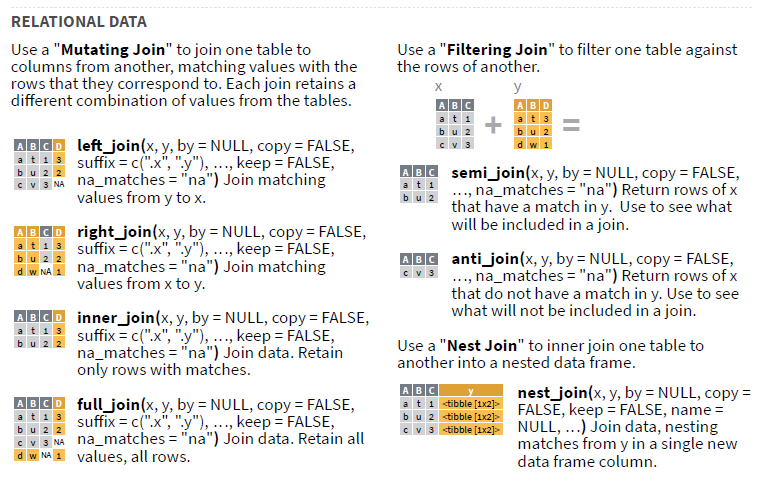
\includegraphics[width=0.6\textwidth,height=\textheight]{./img/joins.PNG}

}

\caption{CC BY SA Posit Software}

\end{figure}

\texttt{left\_join()} og \texttt{right\_join()} er de vi bruker mest, og
vi trenger strengt tatt bare én av dem. Fordi
\texttt{left\_join(x,\ y)\ ==\ right\_join(y,\ x)}. Det handler bare om
retninga du slår sammen (\emph{merge}/\emph{join}). Vanligvis starter vi
med det datasettet som inneholder mest informasjon (\texttt{x}) og slår
sammen et annet datasett (\texttt{y}) oppå dette igjen. Det er ikke
sikkert vi trenger alle radene fra \texttt{y}, derfor gjør vi en
\texttt{left\_join(x,\ y)} som sørger for at alle rader fra \texttt{x}
bevares, pluss alle rader fra \texttt{y} som korresponderer til rader i
\texttt{x}.

La oss se på noen enkle joins. Først genererer jeg et noen datasett som
vi kan bruke. Datasetta inneholder navn på diverse firmaer, og detaljer
rundt disse firmaene.

\begin{Shaded}
\begin{Highlighting}[]
\CommentTok{\# Laster inn en pakke som gir oss tilfeldige navn.}
\FunctionTok{library}\NormalTok{(randomNames)}
\FunctionTok{library}\NormalTok{(tidyverse)}
\end{Highlighting}
\end{Shaded}

\begin{verbatim}
-- Attaching packages --------------------------------------- tidyverse 1.3.2 --
v ggplot2 3.3.6      v purrr   0.3.5 
v tibble  3.1.8      v dplyr   1.0.10
v tidyr   1.2.1      v stringr 1.4.1 
v readr   2.1.3      v forcats 0.5.2 
-- Conflicts ------------------------------------------ tidyverse_conflicts() --
x dplyr::filter() masks stats::filter()
x dplyr::lag()    masks stats::lag()
\end{verbatim}

\begin{Shaded}
\begin{Highlighting}[]
\CommentTok{\# Definer et frø så vi får samme tilfeldige prosess hver gang.}
\FunctionTok{set.seed}\NormalTok{(}\DecValTok{123}\NormalTok{)}

\CommentTok{\# streng med firmasuffikser}
\NormalTok{suffikser }\OtherTok{\textless{}{-}} \FunctionTok{c}\NormalTok{(}\StringTok{"AS"}\NormalTok{, }\StringTok{"og sønner"}\NormalTok{, }\StringTok{"AB"}\NormalTok{, }\StringTok{"firma"}\NormalTok{, }\StringTok{"rørleggere"}\NormalTok{, }\StringTok{"elektrikere"}\NormalTok{, }\StringTok{"blikkenslager"}\NormalTok{, }\StringTok{"ABB"}\NormalTok{, }\StringTok{"og co"}\NormalTok{)}

\CommentTok{\# Hvor mange firma vi skal generere}
\NormalTok{antall }\OtherTok{\textless{}{-}} \DecValTok{20}

\CommentTok{\# La et datasett som inneholder firmanavn, ved å kombinere tilfeldige etternavn}
\CommentTok{\# og suffiksene vi definerte over.}
\NormalTok{firmanavn }\OtherTok{\textless{}{-}} \FunctionTok{tibble}\NormalTok{(}
  \AttributeTok{navn =} \FunctionTok{randomNames}\NormalTok{(antall, }\AttributeTok{which.names =} \StringTok{"last"}\NormalTok{, }\AttributeTok{ethnicity =} \DecValTok{5}\NormalTok{),}
  \AttributeTok{suffiks =} \FunctionTok{sample}\NormalTok{(suffikser, antall, }\AttributeTok{replace =} \ConstantTok{TRUE}\NormalTok{)}
\NormalTok{) }\SpecialCharTok{\%\textgreater{}\%} 
  \FunctionTok{transmute}\NormalTok{(}\AttributeTok{firma =} \FunctionTok{paste}\NormalTok{(navn, suffiks))}

\NormalTok{firmanavn }\SpecialCharTok{\%\textgreater{}\%} \FunctionTok{head}\NormalTok{()}
\end{Highlighting}
\end{Shaded}

\begin{verbatim}
# A tibble: 6 x 1
  firma              
  <chr>              
1 Tanksley og co     
2 Jones blikkenslager
3 Lawrence AB        
4 Riffel ABB         
5 Patterson og co    
6 Warriner AB        
\end{verbatim}

\begin{Shaded}
\begin{Highlighting}[]
\CommentTok{\# Et datasett med inntjening i kr.}
\NormalTok{inntjening }\OtherTok{\textless{}{-}}\NormalTok{ firmanavn }\SpecialCharTok{\%\textgreater{}\%} 
  \FunctionTok{mutate}\NormalTok{(}\AttributeTok{inntekt =} \FunctionTok{round}\NormalTok{(}\FunctionTok{runif}\NormalTok{(antall, }\DecValTok{0}\NormalTok{, }\DecValTok{1000000}\NormalTok{)))}

\NormalTok{inntjening }\SpecialCharTok{\%\textgreater{}\%} \FunctionTok{head}\NormalTok{()}
\end{Highlighting}
\end{Shaded}

\begin{verbatim}
# A tibble: 6 x 2
  firma               inntekt
  <chr>                 <dbl>
1 Tanksley og co        76691
2 Jones blikkenslager  245724
3 Lawrence AB          732135
4 Riffel ABB           847453
5 Patterson og co      497527
6 Warriner AB          387909
\end{verbatim}

\begin{Shaded}
\begin{Highlighting}[]
\CommentTok{\# Et annet datasett med antall ansatte.}
\NormalTok{ansatte }\OtherTok{\textless{}{-}}\NormalTok{ firmanavn }\SpecialCharTok{\%\textgreater{}\%} 
  \FunctionTok{mutate}\NormalTok{(}\AttributeTok{antall =} \FunctionTok{round}\NormalTok{(}\FunctionTok{abs}\NormalTok{(}\FunctionTok{rnorm}\NormalTok{(antall, }\DecValTok{1}\NormalTok{, }\DecValTok{15}\NormalTok{))))}

\NormalTok{ansatte }\SpecialCharTok{\%\textgreater{}\%} \FunctionTok{head}\NormalTok{()}
\end{Highlighting}
\end{Shaded}

\begin{verbatim}
# A tibble: 6 x 2
  firma               antall
  <chr>                <dbl>
1 Tanksley og co          11
2 Jones blikkenslager      8
3 Lawrence AB             13
4 Riffel ABB              11
5 Patterson og co          6
6 Warriner AB              2
\end{verbatim}

Sjølve sammenslåinga er enkel: vi navngir de to datasetta som skal inngå
i sammenslåinga, og hvilken eller hvilke variabler som skal inngå i
sammenslåinga.

\begin{Shaded}
\begin{Highlighting}[]
\NormalTok{firmaoversikt }\OtherTok{\textless{}{-}} \FunctionTok{left\_join}\NormalTok{(inntjening, ansatte, }\AttributeTok{by =} \StringTok{"firma"}\NormalTok{)}
\NormalTok{firmaoversikt }\SpecialCharTok{\%\textgreater{}\%} \FunctionTok{head}\NormalTok{()}
\end{Highlighting}
\end{Shaded}

\begin{verbatim}
# A tibble: 6 x 3
  firma               inntekt antall
  <chr>                 <dbl>  <dbl>
1 Tanksley og co        76691     11
2 Jones blikkenslager  245724      8
3 Lawrence AB          732135     13
4 Riffel ABB           847453     11
5 Patterson og co      497527      6
6 Warriner AB          387909      2
\end{verbatim}

Hvis du skal matche på variabler som ikke heter det samme i begge
datasetta kan du enten

\begin{enumerate}
\def\labelenumi{\arabic{enumi}.}
\tightlist
\item
  endre navnet på en av variablene på forhånd.
\item
  oppgit en \textbf{navngitt vektor} i \texttt{by}.
\end{enumerate}

La oss se et eksempel på det siste alternativet, for det bruker vi ofte.

\begin{Shaded}
\begin{Highlighting}[]
\CommentTok{\# endrer navnet på et av datasettas firma{-}kolonne.}
\FunctionTok{names}\NormalTok{(inntjening) }\OtherTok{\textless{}{-}} \FunctionTok{c}\NormalTok{(}\StringTok{"firmanavn"}\NormalTok{, }\StringTok{"grunker"}\NormalTok{)}

\CommentTok{\# Nå har dette datasettet nytt navn }
\FunctionTok{colnames}\NormalTok{(inntjening)}
\end{Highlighting}
\end{Shaded}

\begin{verbatim}
[1] "firmanavn" "grunker"  
\end{verbatim}

\begin{Shaded}
\begin{Highlighting}[]
\NormalTok{firmaoversikt }\OtherTok{\textless{}{-}} \FunctionTok{left\_join}\NormalTok{(inntjening, }
\NormalTok{                           ansatte,}
                           \AttributeTok{by =} \FunctionTok{c}\NormalTok{(}\StringTok{"firmanavn"} \OtherTok{=} \StringTok{"firma"}\NormalTok{))}
\NormalTok{firmaoversikt}
\end{Highlighting}
\end{Shaded}

\begin{verbatim}
# A tibble: 20 x 3
   firmanavn              grunker antall
   <chr>                    <dbl>  <dbl>
 1 Tanksley og co           76691     11
 2 Jones blikkenslager     245724      8
 3 Lawrence AB             732135     13
 4 Riffel ABB              847453     11
 5 Patterson og co         497527      6
 6 Warriner AB             387909      2
 7 Atkinson blikkenslager  246449      4
 8 Sherrill AB             111096      6
 9 Adelman blikkenslager   389994      8
10 Bates elektrikere       571935      0
11 Meyer rørleggere        216893      3
12 Kidd rørleggere         444768     20
13 Payeur ABB              217991      6
14 Eckhardt AB             502300      6
15 Adamson og sønner       353905      0
16 Sunshine og sønner      649985      7
17 Amos elektrikere        374714      4
18 Waite firma             355445     28
19 Brue AS                 533688      2
20 Timmons elektrikere     740334     19
\end{verbatim}

Vi kan også oppgi flere variabler å matche på ved å simpelthen oppgi
flere variabler i \texttt{by}-argumentet:
\texttt{by\ =\ c("firmanavn",\ "avdeling",\ "fylke")}. Dette funker også
som en navngitt vektor dersom man har ulike kolonnenavn i datasetta:
\texttt{by\ =\ c("firmanavn"\ =\ "navn",\ "avdeling"\ =\ "branch",\ "fylke"\ =\ "fylke")}.
Se mer om navngitte vektorer i Kapittel~\ref{sec-navngitt-vektor}.

\hypertarget{kompliserende-faktorer}{%
\section{Kompliserende faktorer}\label{kompliserende-faktorer}}

Det er ikke alltid like enkelt å slå sammen datasett.

\hypertarget{en-til-mange}{%
\subsection{En til mange}\label{en-til-mange}}

Noen ganger har vi en en-til-mange sammenslåing. I dette eksemplet har
\texttt{datX} en kolonne \texttt{colA} med bokstaver fra a til d.~De
forekommer bare en gang hver. Når vi slår den sammen med \texttt{datY},
hvor det er tre rader per bokstav i \texttt{colA}, blir det sammenslåtte
datasettet å brette ut \texttt{colA} slik vi at får med oss alle
verdiene i \texttt{datY} hvor \texttt{colA} har like elementer i begge
datasetta.

\begin{Shaded}
\begin{Highlighting}[]
\CommentTok{\# Genererer to datasett fulle av tall og bokstaver.}
\NormalTok{datX }\OtherTok{\textless{}{-}} \FunctionTok{tibble}\NormalTok{(}
  \AttributeTok{colA =}\NormalTok{ letters[}\DecValTok{1}\SpecialCharTok{:}\DecValTok{5}\NormalTok{],}
  \AttributeTok{colB =} \FunctionTok{seq}\NormalTok{(}\DecValTok{1}\SpecialCharTok{:}\DecValTok{5}\NormalTok{)}
\NormalTok{)}

\NormalTok{datY }\OtherTok{\textless{}{-}} \FunctionTok{tibble}\NormalTok{(}
  \AttributeTok{colA =} \FunctionTok{rep}\NormalTok{(letters[}\DecValTok{1}\SpecialCharTok{:}\DecValTok{10}\NormalTok{], }\AttributeTok{each =} \DecValTok{3}\NormalTok{), }
  \AttributeTok{colC =} \FunctionTok{c}\NormalTok{(}\DecValTok{10}\SpecialCharTok{:}\DecValTok{39}\NormalTok{)}
\NormalTok{)}

\NormalTok{datX }
\end{Highlighting}
\end{Shaded}

\begin{verbatim}
# A tibble: 5 x 2
  colA   colB
  <chr> <int>
1 a         1
2 b         2
3 c         3
4 d         4
5 e         5
\end{verbatim}

\begin{Shaded}
\begin{Highlighting}[]
\NormalTok{datY}
\end{Highlighting}
\end{Shaded}

\begin{verbatim}
# A tibble: 30 x 2
   colA   colC
   <chr> <int>
 1 a        10
 2 a        11
 3 a        12
 4 b        13
 5 b        14
 6 b        15
 7 c        16
 8 c        17
 9 c        18
10 d        19
# ... with 20 more rows
\end{verbatim}

\begin{Shaded}
\begin{Highlighting}[]
\CommentTok{\# Slår dem sammen via colA.}
\NormalTok{datX }\SpecialCharTok{\%\textgreater{}\%} \FunctionTok{left\_join}\NormalTok{(datY, }\AttributeTok{by =} \StringTok{"colA"}\NormalTok{)}
\end{Highlighting}
\end{Shaded}

\begin{verbatim}
# A tibble: 15 x 3
   colA   colB  colC
   <chr> <int> <int>
 1 a         1    10
 2 a         1    11
 3 a         1    12
 4 b         2    13
 5 b         2    14
 6 b         2    15
 7 c         3    16
 8 c         3    17
 9 c         3    18
10 d         4    19
11 d         4    20
12 d         4    21
13 e         5    22
14 e         5    23
15 e         5    24
\end{verbatim}

Det observante leser kan observere at vi i dette tilfellet kunne tatt
sammenslåinga motsatt vei ved å enten bruke en \texttt{right\_join()}
eller sette \texttt{datyY} som \texttt{x} og vice versa. Da ville vi
lagt på \texttt{datY} sine verdier på \texttt{datX} istedenfor motsatt,
og vi ville ikke tenkt å tenke på \emph{utbrettinga} av \texttt{datX}.
Noen ganger er det likevel denne veien vi vil gå, f.eks. hvis vi
virkelig bare er interessert i observasjoner fra \texttt{x}. Her,
f.eks., tar vi ikke med alle bokstavene som forekommer i \texttt{y}.
Hadde vi valgt å slå sammen \texttt{y} på \texttt{x} ville vi måtte
fjerne disse manuelt seinere. Og det kunne vi fint gjort. Igjen, det er
mange veier til Rom.

\hypertarget{partial-match}{%
\subsection{Partial match}\label{partial-match}}

Det er ofte enklest å slå sammen basert på et tall, som ID. Dette fordi
vi i større grad forventer at ID-er er 1) unike og 2) konsekvente på
tvers av datasetta. Men noen ganger ender vi opp med å matche basert på
navn. For eksempel når vi har ei liste med barnehagenavn som vi vil
bruke til å matche informasjon fra to ulike tabeller. En utfordring som
fort oppstår da er at navna ikke er 100 \% identisk i de to datasetta.
Eksempelvis vil noen skrive barnehagenavnet med ``barnehage'' i navnet,
noen skriver barnehage med stor B, andre med liten, noen feilstaver
kanskje barnehagenavnet, eller kanskje barnehagen har endra navn siden
det ene datasettet blei oppretta. Det er mange grunner til inkonsekvens.
Resultatet er det samme: vi må håndtere det på et vis.

To ulike tilnærminger kan brukes:

\begin{enumerate}
\def\labelenumi{\arabic{enumi}.}
\tightlist
\item
  endre ett eller begge datasetta programmatisk slik at de blir likere
  hverandre. Kanskje vi finner ut at ``barnehage'' ikke er nyttig i et
  barnehagenavn, så vi fjerner alle forekomster av det.
\item
  fuzzy join: ta ibruk funksjoner som lar oss slå sammen datasett basert
  på \textbf{ueksakte matcher}. En slik pakke er \texttt{fuzzy\_join()}.
\end{enumerate}

(Lista er ikke uttømmende. Det er så klart mange andre mulige måter å
gjøre dette på.)

Begge tilnærmingene involverer å bruke regex. I arbeidet med
barnehagekapasitet har jeg brukt slike matcher en del. Der gikk jeg for
tilnærming 1. Det er klare rom for forbedring her, og jeg tror det ville
involvert mer regex.

\hypertarget{den-allsidige-join}{%
\section{Den allsidige join}\label{den-allsidige-join}}

Hovedpoenget med \emph{joins} er å slå sammen datasett fra ulike kilder.
I min kode vil dere se at jeg innimellom har funnet andre bruksområder
for dem. I enkelte tilfeller finnes det sikkert andre måter å løse
problemet på, men den første løsninga jeg fant som virka, var å bruke
\texttt{join}. Og hvis det funker, er det greit. La oss se et eksempel:
Vi har et datasett som viser antall personer i hver alder (fra 0 til
119). Vi har lyst å gjøre om \emph{kontinuerlig} alder til
\emph{alderskategorier} med \emph{fem} alderstrinn i hver kategori opp
til 80. Alle som er 80 eller eldre havner i sin egen kategori. Vi kan
gjøre dette enkelt med en \texttt{mutate()} og \texttt{case\_when()},
men det vil kreve at vi gjentar oss sjøl mer enn tre ganger. Ergo kan vi
spare tid ved å gjøre det per programmatisk.\footnote{Jeg gjorde det
  ikke hver dag.}

\begin{Shaded}
\begin{Highlighting}[]
\CommentTok{\# Simulerer folkemengden i et område, i form av antall personer av hver }
\CommentTok{\# kjønn og hvert alderstrinn.}
\NormalTok{folkemengde }\OtherTok{\textless{}{-}} \FunctionTok{tibble}\NormalTok{(}
  \AttributeTok{alder =} \FunctionTok{c}\NormalTok{(}\FunctionTok{c}\NormalTok{(}\DecValTok{0}\SpecialCharTok{:}\DecValTok{119}\NormalTok{), }\FunctionTok{c}\NormalTok{(}\DecValTok{0}\SpecialCharTok{:}\DecValTok{119}\NormalTok{)),}
  \AttributeTok{kjonn =} \FunctionTok{c}\NormalTok{(}\FunctionTok{rep}\NormalTok{(}\StringTok{"M"}\NormalTok{, }\DecValTok{120}\NormalTok{), }\FunctionTok{rep}\NormalTok{(}\StringTok{"K"}\NormalTok{, }\DecValTok{120}\NormalTok{)),}
  \AttributeTok{antall =} \FunctionTok{round}\NormalTok{(}\FunctionTok{runif}\NormalTok{(}\DecValTok{240}\NormalTok{, }\DecValTok{50}\NormalTok{, }\DecValTok{200}\NormalTok{))}
\NormalTok{)}
\NormalTok{folkemengde}
\end{Highlighting}
\end{Shaded}

\begin{verbatim}
# A tibble: 240 x 3
   alder kjonn antall
   <int> <chr>  <dbl>
 1     0 M         93
 2     1 M         76
 3     2 M         76
 4     3 M        122
 5     4 M         88
 6     5 M         82
 7     6 M        151
 8     7 M         57
 9     8 M        155
10     9 M        103
# ... with 230 more rows
\end{verbatim}

Her er den suboptimale løsninga

\begin{Shaded}
\begin{Highlighting}[]
\NormalTok{folkemengde }\SpecialCharTok{\%\textgreater{}\%} 
  \FunctionTok{mutate}\NormalTok{(}
    \AttributeTok{aldersgruppe =} \FunctionTok{case\_when}\NormalTok{(}
\NormalTok{      alder }\SpecialCharTok{\textless{}} \DecValTok{5} \SpecialCharTok{\textasciitilde{}} \DecValTok{1}\NormalTok{, }
\NormalTok{      alder }\SpecialCharTok{\textgreater{}=} \DecValTok{5} \SpecialCharTok{\&}\NormalTok{ alder }\SpecialCharTok{\textless{}} \DecValTok{10} \SpecialCharTok{\textasciitilde{}} \DecValTok{2}\NormalTok{,}
\NormalTok{      alder }\SpecialCharTok{\textgreater{}=} \DecValTok{10} \SpecialCharTok{\&}\NormalTok{ alder }\SpecialCharTok{\textless{}} \DecValTok{15} \SpecialCharTok{\textasciitilde{}} \DecValTok{3}\NormalTok{,}
      \CommentTok{\# ... osv.}
      \ConstantTok{TRUE} \SpecialCharTok{\textasciitilde{}} \ConstantTok{NA\_real\_}
\NormalTok{    )}
\NormalTok{  )}
\end{Highlighting}
\end{Shaded}

\begin{verbatim}
# A tibble: 240 x 4
   alder kjonn antall aldersgruppe
   <int> <chr>  <dbl>        <dbl>
 1     0 M         93            1
 2     1 M         76            1
 3     2 M         76            1
 4     3 M        122            1
 5     4 M         88            1
 6     5 M         82            2
 7     6 M        151            2
 8     7 M         57            2
 9     8 M        155            2
10     9 M        103            2
# ... with 230 more rows
\end{verbatim}

Og vår smarte løsning som utnytter en \texttt{join}. Vi starter med å
lage aldersgruppene via serier med tall. Dette kan vi gjøre fordi de
første 16 aldersgruppene er like store, de inneholder fem alderstrinn
hver. Vi bruker \texttt{rep()} sammen med \texttt{seq()} for å repetere
hvert ledd i en sekvens fem ganger. Vi legger disse aldersgruppene inn i
et datasett ved siden av kontinuerlig alder. Nå har vi et datasett som
vi rett og slett kan slå sammen med vår opprinnelig datasett. Nøkkelen
blir alder.

\begin{Shaded}
\begin{Highlighting}[]
\CommentTok{\# Legg på alderskategorier {-}{-}{-}{-}}
\CommentTok{\# Vi lager alderskategorier. Deler inn alle aldre i grupper med fem alderstrinn}
\CommentTok{\# i hver. Dette gjør vi ved å fordele hver alder i en kategori, og lime disse}
\CommentTok{\# kategoriene inn i datasettet vårt.}

\CommentTok{\# Lager en serie fra 0 til 119.}
\NormalTok{alder }\OtherTok{\textless{}{-}} \FunctionTok{c}\NormalTok{(}\DecValTok{0}\SpecialCharTok{:}\DecValTok{119}\NormalTok{)}

\CommentTok{\# Lager en serie fra 17 hvor hver kategori repeteres fem ganger. Siste kategori}
\CommentTok{\# repeteres til slutten (alle mellom 80 og 119).}
\NormalTok{aldersgruppe }\OtherTok{\textless{}{-}} \FunctionTok{rep}\NormalTok{(}\FunctionTok{seq}\NormalTok{(}\DecValTok{1}\SpecialCharTok{:}\DecValTok{16}\NormalTok{), }\AttributeTok{each =} \DecValTok{5}\NormalTok{) }\SpecialCharTok{\%\textgreater{}\%} 
  \FunctionTok{c}\NormalTok{(}\FunctionTok{rep}\NormalTok{(}\DecValTok{17}\NormalTok{, }\DecValTok{40}\NormalTok{))}

\CommentTok{\# Putter de to seriene inn i et data.frame slik at vi kan bruke den seinere.}
\NormalTok{alder\_df }\OtherTok{\textless{}{-}} \FunctionTok{tibble}\NormalTok{(}
  \AttributeTok{alder =}\NormalTok{ alder,}
  \AttributeTok{aldersgruppe =}\NormalTok{ aldersgruppe}
\NormalTok{)}

\CommentTok{\# Logikken er at vi merger folkemengde med aldersdatasettet for å få }
\CommentTok{\# overført alderskategoriene våre.}
\NormalTok{folkemengde }\OtherTok{\textless{}{-}}\NormalTok{ folkemengde }\SpecialCharTok{\%\textgreater{}\%} 
  \FunctionTok{left\_join}\NormalTok{(alder\_df, }
            \AttributeTok{by =} \StringTok{"alder"}\NormalTok{)}
\NormalTok{folkemengde}
\end{Highlighting}
\end{Shaded}

\begin{verbatim}
# A tibble: 240 x 4
   alder kjonn antall aldersgruppe
   <int> <chr>  <dbl>        <dbl>
 1     0 M         93            1
 2     1 M         76            1
 3     2 M         76            1
 4     3 M        122            1
 5     4 M         88            1
 6     5 M         82            2
 7     6 M        151            2
 8     7 M         57            2
 9     8 M        155            2
10     9 M        103            2
# ... with 230 more rows
\end{verbatim}

\begin{Shaded}
\begin{Highlighting}[]
\CommentTok{\# Vi kan summere opp  for å vise at vi fikk det til.}
\NormalTok{folkemengde }\SpecialCharTok{\%\textgreater{}\%} 
  \FunctionTok{group\_by}\NormalTok{(kjonn, aldersgruppe) }\SpecialCharTok{\%\textgreater{}\%} 
  \FunctionTok{summarise}\NormalTok{(}\AttributeTok{antall =} \FunctionTok{sum}\NormalTok{(antall)) }\SpecialCharTok{\%\textgreater{}\%} 
  \FunctionTok{print}\NormalTok{(}\AttributeTok{n =} \DecValTok{25}\NormalTok{)}
\end{Highlighting}
\end{Shaded}

\begin{verbatim}
`summarise()` has grouped output by 'kjonn'. You can override using the
`.groups` argument.
\end{verbatim}

\begin{verbatim}
# A tibble: 34 x 3
# Groups:   kjonn [2]
   kjonn aldersgruppe antall
   <chr>        <dbl>  <dbl>
 1 K                1    579
 2 K                2    712
 3 K                3    670
 4 K                4    640
 5 K                5    600
 6 K                6    692
 7 K                7    538
 8 K                8    632
 9 K                9    500
10 K               10    789
11 K               11    675
12 K               12    667
13 K               13    529
14 K               14    570
15 K               15    601
16 K               16    704
17 K               17   4878
18 M                1    455
19 M                2    548
20 M                3    758
21 M                4    601
22 M                5    733
23 M                6    469
24 M                7    700
25 M                8    587
# ... with 9 more rows
\end{verbatim}

Det finnes helt sikkert enda enklere løsninger enn dette, og litt av
gleden av å jobbe i R er å oppdage disse og forbedre gamle syntakser.

\bookmarksetup{startatroot}

\hypertarget{arbeidsprosess}{%
\chapter{Arbeidsprosess}\label{arbeidsprosess}}

Her er noen generelle kommentarer om hvordan prosjektene mine har vært
organisert. Det vil gjøre det lettere for andre å ta over. Her er en
grov oversikt over arbeidsprosessen min, etterfulgt av nøyere detaljer

Hovedenheten i arbeidsprosessen er et prosjekt. Hva et prosjekt er er et
spørsmål jeg syns blir vanskeligere og vanskeligere å svare på desto
lengre jeg holder på med prosjekter. Kort fortalt har de et felles tema,
og noen få, relaterte output. Da kan man gjenbruke koder på tvers av
relaterte skript. Eksempler på prosjekter er arbeidet med
barnehagekapasitet, arbeidet med flyttestatistikk, prognoseevalueringa.
Dette er en abstrakte inndelinga av arbeidet mitt, og det sammenfaller
med den fysiske inndelinga i mapper og Rstudio-prosjekter. Hvert
prosjekt inneholder (vanligvis): et hovedskript og en del støtteskript.
De ligger lagra på \emph{Mine dokumenter} på \texttt{C:}, med oppdaterte
sikkerhetskopier på
\texttt{M:\textbackslash{}StatTK\textbackslash{}R\textbackslash{}sikkerhetskopier}.

\hypertarget{rproj}{%
\section{Rproj}\label{rproj}}

\href{https://support.posit.co/hc/en-us/articles/200526207-Using-RStudio-Projects}{Rstudio-prosjekter}
er en nyttig måte å organisere prosjekter i R. Hovednytten kommer i at
alle filstier blir \emph{relative til prosjektets rotmappe}. Rotmappa er
der \texttt{.Rproj}-fila ligger. Hadde jeg måtte definere alle stier ut
fra hvor de ligger på \emph{min} PC ville det blitt vanskelgiere for
dere å ta over. Pakka \texttt{here} er også nyttig for å gjøre stier
enda mer robuste.

Når vi prater om \texttt{.Rproj}, her er en instilling dere burde endre
på hvis du ikke alt har gjort det: Skru av lagring av workspace mellom
sesjoner. Se beskrivelse i Kapittel~\ref{sec-rstudio}.

Hvis du lurer på om en mappe er et Rstudio-prosjekt kan se se etter en
\texttt{.Rproj}-fil. Legg f.eks. merke til at i mappa \texttt{apps}
inneholder tre undermapper og ingen \texttt{.Rproj}. Dette fordi hver
\emph{app} er sitt eget Rstudio-prosjekt.

\hypertarget{main-filer-og-mappestruktur}{%
\section{main-filer og
mappestruktur}\label{main-filer-og-mappestruktur}}

Generelt etterstreber jeg en mappestruktur som er omtrent slik ut:

\begin{Shaded}
\begin{Highlighting}[]
\NormalTok{.}
\NormalTok{└── mitt\_prosjekt}
\NormalTok{    ├── R}
\NormalTok{    │   ├── main.R}
\NormalTok{    │   └── functions.R}
\NormalTok{    ├── output}
\NormalTok{    │   ├── }\SpecialCharTok{*}\NormalTok{.xlsx}
\NormalTok{    │   └── }\SpecialCharTok{*}\NormalTok{.csv}
\NormalTok{    ├── data}
\NormalTok{    │   ├── }\SpecialCharTok{*}\NormalTok{.xlsx}
\NormalTok{    │   └── }\SpecialCharTok{*}\NormalTok{.csv}
\NormalTok{    ├── README.md}
\NormalTok{    └── .gitignore}
\end{Highlighting}
\end{Shaded}

Ingen prosjekter ser akkurat slik ut, men det er et mål. Elementene i
mappa:

\begin{itemize}
\tightlist
\item
  I mappa \texttt{R} ligger alle kodeskriptene.
\item
  \texttt{main.R}: dette er et lite skript som laster inn funksjoner fra
  andre skript, og som kun inneholder de få kodene som trengs for å lage
  outputen. Vanligvis putter jeg all funksjonalitet inn i funksjoner som
  jeg putter i ett eller flere egne skript.
\item
  \texttt{functions.R}: Om det kun er ett skript, heter dette vanligvis
  \texttt{functions.R}. Blir det mange funksjoner og uoversiktelig med
  alle i ett skript, deler jeg dem opp i flere skript med mer eller
  mindre beskrivende navn som \texttt{cleaning-functions.R},
  \texttt{import-functions.R}, etc.
\item
  I mappa \texttt{output} ligger alle de prosesserte filene. Ofte
  \texttt{.csv} eller \texttt{.xlsx} filer.
\item
  I mapppa \texttt{data} ligger rådatafilene. I noen prosjekter lasta
  jeg ned data fra nettet og la her. Andre plasser lasta jeg ned data
  via API, og lagre en kopi av dem her for å ikke beslaglegge API-en
  unødvendig. I andre kopierte jeg filer fra \texttt{M:}-disken og la
  her. Hvis jeg arbeida med filer fra \texttt{M:} pleide jeg vanligvis å
  oppgi filstien til fila direkte i funksjonen som importerte dataene
  til R.
\item
  Ideelt sett skulle alle prosjekter har en \texttt{readMe.md} (eller
  \texttt{lesMeg.md} på norsk). Denne fila (som noen gang blei printa
  som en pdf) forklarer hva prosjektet handler om.
\item
  \texttt{.gitignore}: denne fila brukes av Git (se ned), og du kan se
  bort fra den.
\end{itemize}

Shiny-appene har i tillegg en fil som heter \texttt{app.R}, som har
samme hovedfunksjon som \texttt{main.R}. Her defineres sjølve appen.
Alle skript som ligger i \texttt{R} blir automatisk kjørt når man kjører
\texttt{app.R}, i motsetning til \texttt{main.R} hvor man manuelt må
kjøre alle skript via \texttt{source()}.

Mange av prosjekta er en eksentrisk blanding av engelsk og norsk, som
kom av at jeg vanligvis koder på engelsk og dokumenterer på norsk. I
enkelte prosjekter var jeg flinkere på være konsekvent enn i andre.

I noen main-filer har jeg kommentert vekk linjer som produserer data som
blir lagra på disk. Dette fordi man kan komme i skade for å kjøre dem
uforvarende og skrive over noe. F.eks. i appen fodte-dode har jeg gjort
dette. Der ligger en funksjon som er tenkt å kjøres en gang i måneden
for å hente nye dødetall via SSBs API.

\hypertarget{git}{%
\section{Git}\label{git}}

Jeg har brukt \textbf{Git} på alle prosjektene. Git er et
\emph{version-control system}, og nyttig når man koder. Jeg har brukt
det for å unngå det vi ser i figuren på
\href{https://peerj.com/preprints/3159v2/}{side 4 av denne artikkelen}:
mange versjoner av samme dokument med ulike navn som indikerer hvilken
versjon det er snakk om. Kort fortalt sørger Git for at jeg \emph{har}
alle disse gamle versjonene av dokumentene tilgjengelig, men at de ikke
\emph{vises} og tar opp plass i mappestrukturen min. Dermed holder jeg
lettere oversikt.

Dere trenger ikke vite noe om Git fordi jeg har sørga for at det alltid
er siste versjon som ligger klar. Jeg nevner det likevel fordi dere kan
lure på hvorfor det ligger noen filer som heter \texttt{.git} og
\texttt{.gitignore} i prosjektene. Disse filene brukes av git. Det kan
slette dem uten at det vil ødelegge prosjektene. (Men da vil all
historikken gå tapt, og det er ikke lengre mulig å se eldre versjoner av
skriptene mine).

Jeg brukte altså Git som en måte å holde orden i filene mine, men også
til å sikkerhetskopiere til M-disken. M er som kjent en server vi kobler
oss på trådløst. Her lagrer vi alt vi arbeider med (som ikke går på
Google disk). Problemet med M er at det er en ekstern server. Dermed kan
enkelte prosesser tar mye lengre tid når man arbeider med filer som
ligger på M. Dessuten vil en del programmer frike ut dersom tilkoblinga
til M blir borte i et mikrosekund, slik den plagsomt nok blir hvis
skjermspareren kommer på eller hvis et atom nyser i feil retning. Min
løsning blei å jobbe med alt på den lokale C-disken og kopiere over alt
til M-disken på slutten av hver dag\footnote{Jeg gjorde det ikke hver
  dag.}. Dette høres tungvint ut, tenker du sikkert. Kopiere over alle
filer til et prosjekt hver dag? Huff. Men det var ikke vanskeligere enn
å skrive inn dette i en konsoll: \texttt{git\ push}.

\hypertarget{hva-muxe5-du-vite-om-git}{%
\subsection{Hva må du vite om Git}\label{hva-muxe5-du-vite-om-git}}

Ingen ting. Det holder å vite at jeg brukte Git, og det er derfor visse
filer eksisterer i prosjektene. Det er smart å la disse ligge der i fall
dere en gang får lyst å bruke Git sjøl. Og for å beholde historikken min
(som jeg tviler på at dere noen gang vil ha nytte av).

Det som ligger i mappa \texttt{R/sikkerhetskopier} på M er essensielt
det samme som ville ligget der dersom jeg hadde manuelt dratt filene
over. Jeg antar at C-disken på pc-en min blir \emph{mind wiped} snart,
og da vil dette være de eneste kopiene av arbeidet mitt, så dere trenger
ikke tenke på hva som er kopi av hva.

\begin{figure}

{\centering 
\includegraphics[width=0.4\textwidth,height=\textheight]{./img/mind-wipe.jpg}

}

\caption{Min pc, snart.}

\end{figure}

\hypertarget{lagringslokasjon}{%
\section{Lagringslokasjon}\label{lagringslokasjon}}

Som jeg nevnt over arbeida jeg på den lokale C-disken, og opprettholdt
sikkerhetskopier på M. For å utbrodere litt på dette: Noen ganger er det
vanskelig å arbeide på filer direkte på en ekstern server. Det er ikke
helt kosekvent hvordan dette utarter seg. I arbeidet med flytterater
skal jeg skrive en excelfil til M-disken. Dette tar flere minutter. Å
skrive den til C-disken tar ett sekund. Og å kopiere fra C til M tar
sekunder. Dermed er det kjappere å skrive fila til C og så kopiere den
til M. R lar oss manipulere filer direkte. Så i denne koden har jeg lagd
en funksjon som kopierer det vi trenger fra M til C, og kopierer det
ferdige produktet tilbake til M fra C. Vi kan gjøre dette relativt
sømløst, slik at brukeren ikke trenger å tenke på hvor filer er lagra.
Så lenge vi sjøl har kontroll, så klart.

Som nevnt tidligere over her og når pakka \emph{here} omtales, i et
prosjekt er alle filstier relative til prosjektets rotmappe. Dermed vil
det ikke oppstå noen problemer når det kommer til filer \emph{som ligger
i en undermappe av prosjektet}. F.eks. legger jeg som nevnt datafiler i
mappa \emph{data}. Uansett hvor du kopierer et prosjekt til, så lenge du
åpner prosjektet i Rstudio skal disse lenkene fungere (til og med om du
åpner dem på en pc med macOS!). Noen filer vi bruker ligger på M. Her er
det viktig at disse filstiene bevares eller oppdateres.

På statistikkmappene er det en konvensjon at filer med datasett er
navngitt etter datoen de blei laga. Det vil si at folkemengdefila jeg
henviser til i skriptet fra mars 2023 ikke er den oppdaterte
folkemengdefila i mai 2024. Her må man gå inn og oppdatere koden med
nytt navn. Hvis man føler seg fancy kan man lage en funksjon som gjetter
seg fram til hva som er den nyeste versjonen av en fil.

\hypertarget{functional-programming}{%
\section{Functional programming}\label{functional-programming}}

Jeg har etterstreba et paradigme som kalles \emph{functional
programming}. Dette er en programmeringsstil hvor vi fokuserer på
funksjoner som gjør alt av endringer på data. Resultatet er lettere å
lese, forstå og debugge. Les mer om det i
\href{http://modern-rstats.eu/functional-programming.html}{Modern R with
the tidyverse}. I praksis vil det si at jeg putter funksjoner sammen i
andre funksjoner som jeg gir beskrivende navn. Dette gjør det lettere å
gruppere sammen databehandlingsfunksjoner. Og dermed også å putte
funksjoner i ulike skriptfiler. Jeg bytta nylig til denne praksisen,
etter å tidligere ha arbeida med meterlange skript hvor objekter
opprettes, endres, slettes, transformeres og lagres om hverandre. Så
langt syns jeg dette er en stor forbedring. Utfordringa er å finne en
god balanse mellom hvor mange skript man skal lage, og hvor mange
delfunksjoner man trenger. Du vil se at jeg er inkonsekvent i de ulike
prosjekta mine. Her finnes heller ingen \emph{one size fits all}. Små
prosjekter trenger ikke mer enn en \texttt{main.R}-fil. Store prosjekter
kan ha mange skript fordelt over flere mapper.

\bookmarksetup{startatroot}

\hypertarget{sec-feil}{%
\chapter{Typiske feil vi (jeg) gjør og hvordan fikse
dem}\label{sec-feil}}

Det er uendelig mange måter å gjøre noe feil på. Dette gjelder egentlig
uansett hvilket program du arbeider i. Noe som er fint i R er at du
vanligvis får en klar feilmelding når noe går galt. Noe som er mindre
fint er at denne feilmeldinga ikke alltid er så enkel å tolke. Likevel,
se alltid på meldinga først. Her får du en tydlige pekepinn på hva som
gikk galt. Man lærer seg etter hvert hvordan å lese disse meldingene,
skjønt de kan virke gresk i starten.

Her har jeg samla noen av de feila som jeg enten gjør oftest, eller som
jeg tenker mange gjør feil. Hvis ingenting av dette hjelper, kan man
alltids spørre om hjelp online. Mitt foretrukne nettsted for dette er
\href{https://stackoverflow.com/}{StackOverlow}. Undersida deres,
\href{https://stats.stackexchange.com/}{CrossValidated}, kan også
brukes. Kvaliteten på meldingene her er høy, men det går tidvis på
bekostning av normal høflighet. Hvis man følger reglene deres og gir et
\href{https://reprex.tidyverse.org/}{representativt eksempel} vil de
vanligvis være greie. Dette er forøvrig en bra måte å be om hjelp på
uansett.

\begin{enumerate}
\def\labelenumi{\arabic{enumi}.}
\tightlist
\item
  Forklar tydlig hva du lurer på: hva ønsker du å få som utfall?
\item
  Forklar hva du hva forsøkt
\item
  Gi eksempeldatasett slik at hjelperne kan bruke det når de gir råd
\end{enumerate}

Uansett, her er min liste over typiske feil

\hypertarget{glemt-uxe5-laste-inn-en-pakke}{%
\section{Glemt å laste inn en
pakke}\label{glemt-uxe5-laste-inn-en-pakke}}

Jeg starter alle R-sesjoner med å laste inn pakker, og jeg laster nesten
alltid inn \texttt{tidyverse}. Hvis jeg glemmer det, vil funksjoner fra
denne pakka ikke være tilgjengelig.

\hypertarget{laster-inn-pakker-i-feil-rekkefuxf8lge}{%
\section{Laster inn pakker i feil
rekkefølge}\label{laster-inn-pakker-i-feil-rekkefuxf8lge}}

Det lønner seg å laste inn pakker i omvendt prioritert rekkefølge. Dette
er fordi en del pakker inneholder funksjoner med samme navn, men
\emph{ulik bruksområde}. Da vil den \emph{siste} pakka du laster inn
\emph{maskere} den tidligere funksjonen. For eksempel inneholder
\texttt{stats} funksjonen \texttt{filter()}. Denne blir erstatte med
\texttt{dplyr}s \texttt{filter()} når vi laster inn den pakka (often via
\texttt{tidyverse}). Jeg pleier dermed ofte å laste inn
\texttt{tidyverse} sist. Denne feilen er vanskelig å feilsøke, fordi du
kan få en feilmelding uten å ha gjort noe som helst endring i koden.
(Les: jeg har kasta bort mye tid på å feilsøke når det viste seg at det
eneste jeg hadde gjort var å endre rekkefølgene pakkene blei lasta inn
på, slik an funksjon jeg var avhengig av fra pakke1 blei bytta ut med en
annen funksjon med samme navn fra pakke2.)

Husk at det går an å bruke en pakkes funksjon uten å laste den inn ved å
bruke \texttt{::}, slik som i \texttt{dplyr::filter()}. Det bidrar til
at å unngå at du får lasta inn for mange pakker som overskriver
hverandres funksjoner. Spesielt hvis du bare bruker få funksjoner noen
få ganger, kan dette lønne seg. Jeg gjør vanligvis dette når jeg
importerer datasett, siden dette er noe jeg kun gjør én gang per
prosjekt. Hvis jeg derimot skal eksportere mange filer, vil det spare
tastaturet mitt å bare laste inn pakka.

Forøvrig har vi en liknende feil

\hypertarget{jeg-har-ikke-gjort-noen-endringer-men-plutselig-funker-ikke-koden-min}{%
\section{``Jeg har ikke gjort noen endringer, men plutselig funker ikke
koden
min!''}\label{jeg-har-ikke-gjort-noen-endringer-men-plutselig-funker-ikke-koden-min}}

Dette er i prinsippet umulig å feilsøke. Heldigvis kan vi benytte oss av
et smertelig nyttig prinsipp: Årsaken er alltid at du har gjort en feil.

Dette skjer typisk dersom du har arbeida lenga i en sesjon uten å
restarte R. Første gang du restarter R og kjører koden på nytt får du
feilmelding. Da er ofte problemet at du på et tidspunkt har lagra noe i
miljøet (\emph{environment}), som ikke lengre er tilstede i koden. Hvis
andre deler av koden er avhengig av dette objektet, vil de feile nå som
objektet ikke lengre er tilstede. Du må rett og slett finne ut hvor
bruddet skjer, og fikse det.

En måte å forebygge dette på er ved å ta i bruke \emph{functional
programming}. Det vil si at vi bruker funksjoner i stor grad og sjelden
lagrer objekter direkte i miljøet.
\href{https://www.brodrigues.co/blog/2022-05-26-safer_programs/}{Brodrigues}
forklarer det bedre.

\hypertarget{sender-et-objekt-via-pipe-til-en-funksjon-som-ikke-er-pipevennlig}{%
\section{Sender et objekt via pipe til en funksjon som ikke er
pipevennlig}\label{sender-et-objekt-via-pipe-til-en-funksjon-som-ikke-er-pipevennlig}}

\hypertarget{glemmer-uxe5-bruke-hermetegn-bruker-hermetegn-nuxe5r-vi-ikke-trenger-hermetegn}{%
\section{Glemmer å bruke hermetegn / bruker hermetegn når vi ikke
trenger
hermetegn}\label{glemmer-uxe5-bruke-hermetegn-bruker-hermetegn-nuxe5r-vi-ikke-trenger-hermetegn}}

Her varierer det nok ut ifra hvor god man er på å forstå strukturer. Jeg
gjør denne feilen stadig. Har ikke noe bedre råd enn å alltid prøve
begge veier. Det er så klart smart å finne ut av \emph{hvorfor} man noen
ganger bruker hermetegn rundt noe og andre ganger ikke. Essensielt
handler det om: Når du bruker hermetegn rundt noe viser du at det er en
tekststreng. Når du ikke bruker hermetegn rundt tekst viser du at et er
et objekt. Da må objektet finnes i miljøet for at det skal kunne tas i
bruk. \texttt{tidyverse} kompliserer dette litt ved at de lar oss
henvise til f.eks. kolonnenavn som om de er objekter, f.eks. i:

\begin{Shaded}
\begin{Highlighting}[]
\FunctionTok{library}\NormalTok{(tidyverse)}
\end{Highlighting}
\end{Shaded}

\begin{verbatim}
-- Attaching packages --------------------------------------- tidyverse 1.3.2 --
v ggplot2 3.3.6      v purrr   0.3.5 
v tibble  3.1.8      v dplyr   1.0.10
v tidyr   1.2.1      v stringr 1.4.1 
v readr   2.1.3      v forcats 0.5.2 
-- Conflicts ------------------------------------------ tidyverse_conflicts() --
x dplyr::filter() masks stats::filter()
x dplyr::lag()    masks stats::lag()
\end{verbatim}

\begin{Shaded}
\begin{Highlighting}[]
\CommentTok{\# Ok}
\NormalTok{starwars }\SpecialCharTok{\%\textgreater{}\%} 
  \FunctionTok{select}\NormalTok{(name)}
\end{Highlighting}
\end{Shaded}

\begin{verbatim}
# A tibble: 87 x 1
   name              
   <chr>             
 1 Luke Skywalker    
 2 C-3PO             
 3 R2-D2             
 4 Darth Vader       
 5 Leia Organa       
 6 Owen Lars         
 7 Beru Whitesun lars
 8 R5-D4             
 9 Biggs Darklighter 
10 Obi-Wan Kenobi    
# ... with 77 more rows
\end{verbatim}

\begin{Shaded}
\begin{Highlighting}[]
\CommentTok{\# Feilmelding}
\NormalTok{starwars[name]}
\end{Highlighting}
\end{Shaded}

\begin{verbatim}
Error in `[.tbl_df`(starwars, name): object 'name' not found
\end{verbatim}

\begin{Shaded}
\begin{Highlighting}[]
\CommentTok{\# OK}
\NormalTok{starwars[}\StringTok{"name"}\NormalTok{]}
\end{Highlighting}
\end{Shaded}

\begin{verbatim}
# A tibble: 87 x 1
   name              
   <chr>             
 1 Luke Skywalker    
 2 C-3PO             
 3 R2-D2             
 4 Darth Vader       
 5 Leia Organa       
 6 Owen Lars         
 7 Beru Whitesun lars
 8 R5-D4             
 9 Biggs Darklighter 
10 Obi-Wan Kenobi    
# ... with 77 more rows
\end{verbatim}

Denne kompliseringa godtar vi, for det er så mange fordeler med at
\texttt{tidyverse} lar oss henvise direkte til kolonner i datasett som
om de var objekter.

\hypertarget{feil-skruxe5strek}{%
\section{Feil skråstrek}\label{feil-skruxe5strek}}

Windows vs.~mac Se Kapittel~\ref{sec-slash}.

\hypertarget{tegnkode}{%
\section{Tegnkode}\label{tegnkode}}

Se Kapittel~\ref{sec-tegnkoding}.

Ofte hjelper det å restarte R-sesjonen.

\bookmarksetup{startatroot}

\hypertarget{referanser}{%
\chapter*{Referanser}\label{referanser}}
\addcontentsline{toc}{chapter}{Referanser}

\markboth{Referanser}{Referanser}

En serie med nyttig ressurser og sider å drive produktiv
prokrastinering.

\hypertarget{ressurser-for-uxe5-luxe6re-r}{%
\section*{Ressurser for å lære R}\label{ressurser-for-uxe5-luxe6re-r}}
\addcontentsline{toc}{section}{Ressurser for å lære R}

\markright{Ressurser for å lære R}

R for data science

Advanced R

Swirl

What They Forgot to Teach You About R

Posits cheat sheets

\hypertarget{produktiv-prokrastinering}{%
\section*{Produktiv prokrastinering}\label{produktiv-prokrastinering}}
\addcontentsline{toc}{section}{Produktiv prokrastinering}

\markright{Produktiv prokrastinering}

Brodrigues

Rweekly

Rbloggers



\end{document}
